% WACV 2027 -- Applications Track
% Empirical study: video vs. EEG deep learning (head-to-head, not fused) for
% rodent seizure detection and severity grading. The literature survey lives in the
% supplementary material (sec/9_supplement.tex).
% Modular project: content lives in sec/*.tex; references in main.bib.

\documentclass[10pt,twocolumn,letterpaper]{article}

% wacv.sty loads xcolor[dvipsnames]; pre-pass `table' so \rowcolor works.
\PassOptionsToPackage{table}{xcolor}

%%%%%%%%% PAPER TYPE  - PLEASE UPDATE FOR FINAL VERSION
\usepackage[review,applications]{wacv}   % REVIEW version, Applications track
% \usepackage[review,algorithms]{wacv}   % REVIEW version, Algorithms track
% \usepackage{wacv}                       % CAMERA-READY (shows author block below)
% \usepackage[pagenumbers]{wacv}          % arXiv-style: camera-ready + page numbers

% Additional packages (before hyperref)
%
% preamble.tex -- additional packages, loaded by main.tex after wacv.sty and
% before hyperref. (xcolor is loaded by wacv.sty with [dvipsnames]; the `table'
% option is pre-passed in main.tex so \rowcolor works.)
%

% --- figures, math, tables
\usepackage{graphicx}
\usepackage{amsmath,amssymb}
\usepackage{booktabs}
\usepackage{array}
\usepackage{multirow}
\usepackage{enumitem}   % compact list spacing (itemize/enumerate options)
\usepackage{tikz}       % pipeline / flow diagram
\usetikzlibrary{arrows.meta,positioning,backgrounds,fit,shapes.geometric,calc}
\usepackage{pgfplots}   % result charts (scatter / line / bar plots)
\pgfplotsset{compat=1.18}

% --- Fonts: tectonic compiles with XeTeX, whose Unicode (TU) encoding has no
% bold/italic shape for the kit's Type1 Times (ptm) -> \textbf/\textit silently
% render non-bold. TeX Gyre Termes / Heros are Times/Helvetica clones with the
% full set of OpenType shapes, restoring bold and italic.
\usepackage{iftex}
\ifXeTeX
  \usepackage{fontspec}
  \setmainfont{texgyretermes}[
    Extension=.otf, UprightFont=*-regular, BoldFont=*-bold,
    ItalicFont=*-italic, BoldItalicFont=*-bolditalic]
  \setsansfont{texgyreheros}[
    Extension=.otf, UprightFont=*-regular, BoldFont=*-bold,
    ItalicFont=*-italic, BoldItalicFont=*-bolditalic]
\fi

% --- Teaser pipeline (Figure 1), emitted at the top of page 1 ---------------
% wacv's \maketitle wraps \@maketitle in \twocolumn[...]; the page-1 top region
% is thus title matter and a figure* float declared in the body defers to page 2.
% We inject the full-width pipeline into that top matter so it lands at the very
% top of page 1, above the abstract, numbered Figure~1. Its counter step and
% \label{fig:pipeline} are done in the body (top of sec/1_intro) for pass-stable
% numbering; the caption number is therefore hardcoded "Figure~1.".
\newcommand{\pipelineteaser}{%
  \vspace{0pt}\par\noindent
  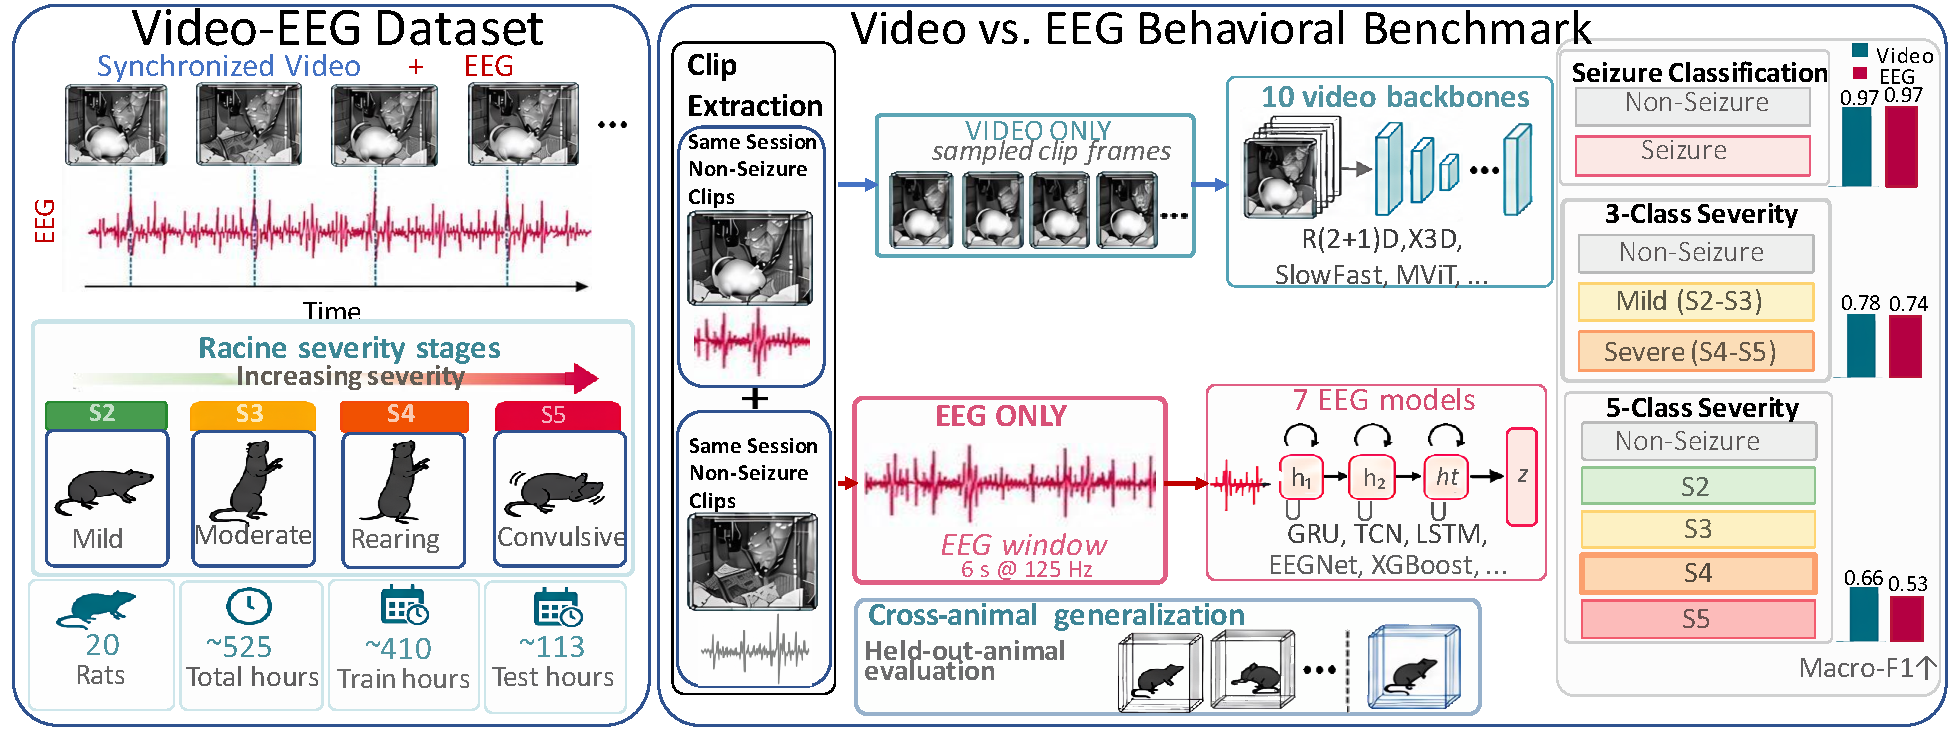
\includegraphics[width=\textwidth]{fig/fig_pipeline.pdf}%
  \par\vspace{2pt}
  {\small Figure~1.\hspace{0.5em}Overview of the study. \emph{Left:} the cohort---
  synchronized video and EEG from 20 rats (corpus scale in
  App.~\ref{sec:dataextra:cohort}, Table~\ref{tab:corpusscale}), each clip graded on the
  Racine scale from Stage\,2 (mild) to Stage\,5 (convulsive). \emph{Right:} the
  benchmark. Expert-annotated seizure clips and same-session non-seizure clips feed
  two independent, unfused lanes---ten video backbones and seven EEG models---%
  compared head-to-head at 2-, 3- and 5-class granularity and under
  held-out-animal evaluation. Bars report macro-F1: the two modalities are level
  at detection and separate as the task becomes explicitly behavioral.\par}%
  \vspace{3pt}%
}
% Append the teaser pipeline to the (two-column-spanning) title top matter.
\makeatletter
\g@addto@macro\@maketitle{\pipelineteaser}
\makeatother

% --- Key-takeaway callout -------------------------------------------------
% A tinted box closing each results subsection with its one-line conclusion.
% Colour matches wacvblue (main.tex), redefined here since preamble is input first.
\usepackage[most]{tcolorbox}
\definecolor{takeawayaccent}{rgb}{0.21,0.49,0.74}
\newtcolorbox{takeaway}{
  enhanced,
  colback=takeawayaccent!6, colframe=takeawayaccent!55,
  boxrule=0.5pt, arc=2pt,
  left=5pt, right=5pt, top=3.5pt, bottom=3.5pt,
  before skip=6pt, after skip=6pt,
  fontupper=\small,
}
\newcommand{\takeawaylabel}{\textbf{\textcolor{takeawayaccent!80!black}{Key takeaway.}}\ }

% --- inline annotations (from the kit)
\newcommand{\red}[1]{{\color{red}#1}}
\newcommand{\todo}[1]{{\color{red}#1}}
\newcommand{\TODO}[1]{\textbf{\color{red}[TODO: #1]}}
% --- disable by uncommenting
% \renewcommand{\TODO}[1]{}
% \renewcommand{\todo}[1]{#1}


% hyperref last
\definecolor{wacvblue}{rgb}{0.21,0.49,0.74}
\usepackage[pagebackref,breaklinks,colorlinks,allcolors=wacvblue]{hyperref}

%%%%%%%%% PAPER ID  - PLEASE UPDATE
\def\wacvPaperID{*****} % *** Enter the WACV Paper ID here
\def\confName{WACV}
\def\confYear{2027}

%%%%%%%%% TITLE
\title{Seeing Seizures: A Large-Scale Empirical Study of Video and EEG
Deep Learning for Automated Rodent Seizure Detection and Severity Grading}

%%%%%%%%% AUTHORS (shown only in camera-ready / pagenumbers builds)
\author{Anonymous WACV Applications Track submission}

\begin{document}
\maketitle

\begin{abstract}
Video and EEG are widely used to study seizures in animals. However, manual
scoring remains a huge bottleneck. Making this automatic is a big challenge that
few have solved for animal models. This study tackles the problem using data from
twenty rats, analyzing about 24000 paired clips from 601 sessions. Experts graded
the seizures from a mild Stage\,2 to a severe Stage\,5. Ten video models and seven
EEG models were tested under strict rules to see how well they could spot seizures
and grade their exact severity. For basic detection, both tools did well, while
EEG was slightly better, scoring 0.974 compared to video's 0.968. Both tools also
worked well on unseen rats. The gap grew when grading the exact seizure levels. In
the five-level test, video scored 0.657, easily beating EEG's 0.560. The two
methods also made different types of mistakes. Video usually just confused stages
that were next to each other. EEG was more likely to miss seizures entirely or mix
up very different stages. The size of the video model did not matter much. A tiny
model did almost as well as a huge one. Instead, tracking motion over time was the
real key. An additional test on the outside RodEpil dataset confirmed these
results, with the model score reaching 0.979. Overall, we demonstrate that cameras
offer a great, pain-free way to track animal seizures and work very well alongside
typical EEG tools.
\end{abstract}

% Pipeline teaser (Figure 1) is emitted into the title top matter via
% \pipelineteaser (preamble.tex). Its counter step + label live here in the body
% for pass-stable numbering: teaser pipeline = Fig. 1. The next two body floats
% are declared below so that they print on p.2, next to their first mention in
% the contributions list: fig:setup (Fig. 2) and fig:efficiency (Fig. 3). They
% are discussed in full in Secs. 3 and 5.
\refstepcounter{figure}\label{fig:pipeline}

\section{Introduction}
\label{sec:intro}

Epilepsy affects roughly 1\% of the world's population~\cite{liu2026}. Almost
everything we know about its mechanisms, and every candidate anti-seizure
therapy, is first established in animal models, predominantly chemically or
electrically induced rodents~\cite{bhatt2021}. These studies rest on
\emph{synchronized video--EEG}: an overhead camera records behavior while
implanted electrodes record cortical activity. The two modalities are
complementary. Electrographic seizures can occur with little visible movement,
and movement artifacts routinely corrupt the EEG, so an experimenter confirms
that an event is a seizure, and grades its behavioral severity on the Racine
scale, only by reading both channels together~\cite{racine1972, lundt2015}. This
complementarity makes video--EEG the gold standard of preclinical epilepsy
research~\cite{bhatt2021}.

Manual scoring makes this rigor expensive. A single study can generate thousands
of hours of paired video and EEG, and a trained annotator reviews all of it.
Automating the behavioral half of this workflow is a \emph{video-understanding}
problem: modern action-recognition
backbones~\cite{carreira2017i3d,tran2018r2plus1d,feichtenhofer2019slowfast} and
animal pose estimators~\cite{mathis2018deeplabcut,pereira2022sleap} are mature
and transferable. Yet the epilepsy literature has been slow to adopt them,
especially in animal studies. Video-only rodent detection has only just acquired
its first public benchmark~\cite{rodepil2025}, and computational video--EEG
fusion in animals is confined to two isolated \emph{binary}
detectors~\cite{mullen2024,eegvfusion2026}, neither grading severity. No one has yet measured \emph{how far standard video deep learning actually gets}
on this problem against a strong EEG reference on the same data.

% --- p.2 floats: acquisition, one synchronized pair, and the headline
% efficiency result. Declared here (rather than in Secs. 3-5, where each is
% discussed) so they print beside their first mention in the contributions list.
\begin{figure}[t]
\centering
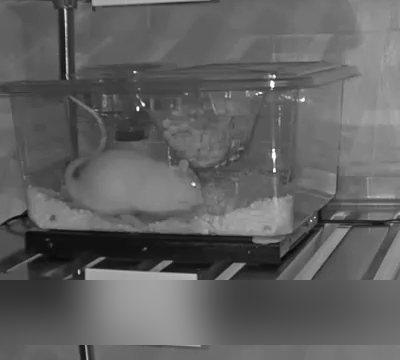
\includegraphics[width=0.60\linewidth]{fig/stages/f_setup.png}
\caption{A representative overhead frame of the acquisition setup: each rat is
recorded in its home cage by a fixed overhead camera while implanted electrodes
stream synchronized EEG, and the cage rests on a per-animal platform. Camera
geometry differs per cage, so clips are per-cage cropped before subjects are
pooled. De-identified (cage-side identifier redacted).}
\label{fig:setup}
\end{figure}

% fig:paired now lives in sec/2_related.tex so it prints on the Related Work page
% beside the multimodal video--EEG paragraph it illustrates.

\begin{figure}[t]
\centering
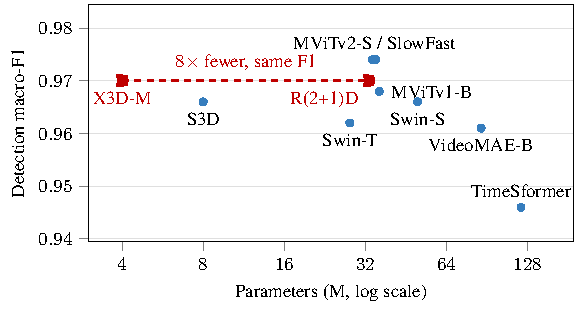
\includegraphics[width=\linewidth]{fig/fig_efficiency.pdf}
\caption{Detection accuracy \vs\ model size across ten video backbones (accuracies from
Table~\ref{tab:vidarch}, parameter counts from Table~\ref{tab:vidspec}). Every
architecture lands in a narrow 0.946--0.974 macro-F1 band, and the 4M-parameter
X3D-M ties the 33M R(2+1)D-18 at 0.970, an $8\times$ saving at no cost in
accuracy.}
\label{fig:efficiency}
\end{figure}

This paper provides that account. The contribution is empirical: on a real
preclinical cohort, under a single controlled protocol, we report where a standard video backbone matches EEG,
where it surpasses it, where it breaks, and how the choice of architecture,
temporal sampling, data budget and evaluation protocol shape the answer. A
comprehensive literature survey of the field (video-only and multimodal
video--EEG detection across human and animal subjects) is provided in the
supplementary material (App.~\ref{sec:survey}); the main paper is the empirical
study.

We organize that study around four questions:
\begin{itemize}[leftmargin=2.6em,itemsep=1pt,topsep=2pt]
  \item[\textbf{RQ1}] \emph{What model and input capacity is sufficient?}
  (Sec.~\ref{sec:rq1})
  \item[\textbf{RQ2}] \emph{Do the two modalities fail in the same way, or are
  their errors complementary?} (Sec.~\ref{sec:crossmodal})
  \item[\textbf{RQ3}] \emph{Once a seizure is identified, does ordinal modeling
  improve Stage\,2--5 grading and reduce large-stage errors on unseen subjects?}
  (Sec.~\ref{sec:problem:ordinal})
  \item[\textbf{RQ4}] \emph{Does inverse-frequency weighting keep the long tail
  from dominating the result?} (Sec.~\ref{sec:rq3})
\end{itemize}
All four rest on the head-to-head comparison itself: how far a standard
video backbone gets against an electrode-based reference, and whether that ordering
survives held-out animals and an external benchmark
(Sec.~\ref{sec:crossmodal}). Our contributions are:

\begin{itemize}
  \itemsep0.15em
  \item A \textbf{pooled twenty-subject synchronized video--EEG cohort}
  (Sec.~\ref{sec:data}): $\sim$24k expert-annotated, per-cage-cropped clips over
  601 sessions with per-clip Racine severity labels and severely long-tailed
  burden. To our knowledge this is the largest paired rodent video--EEG corpus
  studied for learned detection. Figure~\ref{fig:setup} shows the acquisition setup: one
  fixed overhead camera per home cage, so geometry is constant within an animal and
  differs across animals, which is why we crop per cage. We release a fully
  de-identified description.
  \item A \textbf{head-to-head video-\vs-EEG comparison} across three task
  granularities (Sec.~\ref{sec:application}) under a matched, leakage-controlled
  protocol. Video matches a strong EEG reference on detection (0.993 \vs\ 0.992
  AUROC) and degrades far more gracefully on severity grading, with Grad-CAM
  evidence that the model attends to behaviorally meaningful regions.
  \item A \textbf{controlled sweep of ten video backbones and seven EEG models},
  plus temporal-sampling, resolution, data-efficiency and pretraining ablations.
  Detection is backbone-agnostic on this cohort (Fig.~\ref{fig:efficiency}):
  accuracy is flat in model size, and a 4M-parameter X3D matches a 33M R(2+1)D.
  Temporal context is what matters: a single-frame control collapses at
  every granularity (0.569 macro-F1 at detection against 0.970 at 16 frames),
  which shows the task is read from motion. Under \textbf{subject-disjoint}
  cross-validation the two modalities stay level at detection, while video's
  advantage at 3- and 5-class grading holds.
  \item \textbf{External validation} on the public RodEpil
  benchmark~\cite{rodepil2025} (0.979 subject-wise F1), together with a
  documented encoding artifact in its raw release that must be corrected for an
  honest score.
\end{itemize}

\section{Related Work}
\label{sec:related}

Efforts to automate seizure scoring divide by the signal they read. We position our
study against three such lines, each treated at length in the
supplementary survey (App.~\ref{sec:survey}). That survey is organized by modality,
covering EEG-only (App.~\ref{sec:eeg}), video-only (App.~\ref{sec:video}) and fused
video--EEG (App.~\ref{sec:fusion}) work, and by subject (human \vs\ animal). Its gap
analysis (App.~\ref{sec:taxonomy}, Table~\ref{tab:gap}) locates our contribution.

% Declared here so the float prints on the Related Work page, beside the
% multimodal video--EEG paragraph that first cites it.
\begin{figure}[t]
\centering
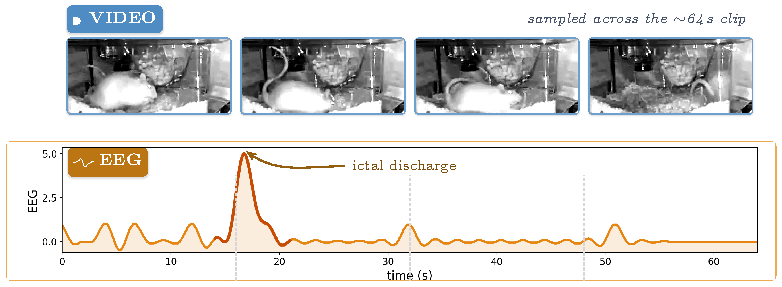
\includegraphics[width=\linewidth]{fig/fig_paired.pdf}
\caption{Synchronized video--EEG for one Stage-3 seizure clip (subject R7). \emph{Top:}
four frames sampled across the clip (contrast-enhanced), aligned to the shared time
axis. \emph{Bottom:} the simultaneous single-channel EEG ($\sim$64\,s), the shaded
window marking the ictal discharge. Video carries the convulsive motion, EEG the
electrographic discharge; this pairing is what our study rests on. De-identified.}
\label{fig:paired}
\end{figure}

\noindent\textbf{EEG-only detection} is the incumbent and sets the accuracy bar.
Rodent systems have moved from hand-crafted spectral features with classical
classifiers~\cite{bergstrom2013} to end-to-end deep networks: spectrogram CNNs
over thousands of hours~\cite{martin2023} and recurrent GRU/LSTM models that
outperform Random Forest and XGBoost on chemically diverse
cohorts~\cite{ganguly2025}. All operate on EEG alone and discard the synchronized
video recorded alongside it. We adopt this family as a deliberately strong seven-model EEG reference for our
cross-modal comparison: a GRU, an LSTM, EEGNet, an EEG Conformer, a TCN, and the
two classical baselines.

\noindent\textbf{Video-only seizure detection} reframes the task as action
recognition, inheriting mature video-understanding backbones (two-stream, 3D and
(2+1)D convolutions, and video transformers~\cite{simonyan2014twostream,
carreira2017i3d,tran2018r2plus1d,feichtenhofer2019slowfast,
bertasius2021timesformer,tong2022videomae}; reviewed in App.~\ref{sec:backbones})
and animal pose
estimators~\cite{mathis2018deeplabcut,pereira2022sleap}. Clinical video systems
target \emph{binary} recognition~\cite{ahmedt2018,karacsony2020seizure,vsvig2024};
in rodents, camera-only detectors have been built for PTZ-induced
mice~\cite{sabnis2024}, chronic-epilepsy screening~\cite{epidetect2024}, home-cage
behavioral monitoring~\cite{jankovic2019homecage} and further mouse~\cite{khan2024mice}
and zebrafish~\cite{whytefagundes2025zebrafish} preparations, and
Perlo~\etal\ recently released \emph{RodEpil}~\cite{rodepil2025}, the first public
video-only rodent benchmark (13{,}053 clips, 19 rats) with a TimeSformer baseline
at 97\% F1 under subject-wise cross-validation. We validate our backbone on
RodEpil directly and extend beyond binary detection to severity grading.

\noindent\textbf{Multimodal video--EEG fusion} is the clinical gold standard.
Figure~\ref{fig:paired} shows the two streams on one clip from our cohort: the
convulsive motion in the frames and the ictal discharge in the trace mark the same
event, and an expert confirms a seizure only by reading them together.
Computationally the pairing is rare, however: only a handful of human studies fuse
both streams~\cite{aghaei_video_eeg,martini2021,cao2024,vepinet2024}, and in animals
just two isolated attempts: late fusion of video, ECoG and piezo in
rats~\cite{mullen2024}, and cross-attention alignment of self-supervised EEG and
video in mice~\cite{eegvfusion2026}. Both address only \emph{binary} detection;
neither grades severity, the harder three- and five-class problem we study. We leave fusion to future work (Sec.~\ref{sec:open}); our aim here is to establish
how far each single modality gets on its own.

\section{Problem Setup}
\label{sec:problem}

We now state the detection and grading problem formally, fixing the notation and
evaluation protocol used throughout our experiments (Sec.~\ref{sec:application}).
Figure~\ref{fig:pipeline} summarizes the pipeline.

\subsection{Flat multi-class formulation}
\label{sec:problem:flat}

\noindent\textbf{Clips and labels.}
A recording session provides temporally synchronized video and EEG. Around each
expert-annotated event we extract a clip $c=(\mathbf{V},\mathbf{E})$, where
$\mathbf{V}\in\mathbb{R}^{T\times H\times W\times 3}$ is a short RGB video segment
and $\mathbf{E}\in\mathbb{R}^{C\times L}$ the corresponding $C$-channel EEG trace.
Matched non-seizure clips are sampled from seizure-free intervals of the same
sessions. Each clip carries a severity label $y\in\{0,1,2,3,4\}$: $0$
denotes non-seizure and $1$--$4$ the ictal stages (Racine~\cite{racine1972}
Stage\,2--5). Racine Stage\,1 (mouth and facial automatisms) is annotated in this
cohort but occurs in only six clips, too few to train or evaluate a class on, so we
exclude it. The modeled label space begins at Stage\,2 as a consequence of the
data, and not because the scale starts there. The scale itself was derived from electrically
kindled seizures, and its transfer to chemically induced models is not
automatic~\cite{vanerum2019racine}; we use the grades our annotator assigned and do not re-derive a
model-specific scale. Each clip also belongs to a subject $s\in\mathcal{S}$ and a session
$r\in\mathcal{R}$. The corpus pools clips from all subjects.
Figure~\ref{fig:setup} shows a representative frame of the recording setup;
because camera geometry differs per cage, each clip is cropped per cage before
subjects are pooled.

% fig:setup now lives in sec/1_intro.tex so it prints on p.2 alongside its first
% mention in the contributions list.

\noindent\textbf{Task granularities.}
We study three classification tasks of increasing difficulty, each obtained by
collapsing the stage label through a map $g_k:\{0,\dots,4\}\to\{0,\dots,k-1\}$:
\begin{itemize}[leftmargin=1.2em,itemsep=1pt,topsep=2pt]
  \item \textbf{Detection} ($k{=}2$): $g_2(y)=\mathbf{1}[y>0]$: seizure \vs\
        non-seizure.
  \item \textbf{Coarse grading} ($k{=}3$): non-seizure / mild (Stage\,2--3) /
        severe (Stage\,4--5).
  \item \textbf{Fine grading} ($k{=}5$): the full non-seizure / Stage\,2--5 scale.
\end{itemize}

\noindent\textbf{Modalities.}
Each task pairs two \emph{unimodal} predictors that we compare head-to-head:
a video model $f_{\mathrm{V}}:\mathbf{V}\mapsto\hat{y}$ and an EEG model
$f_{\mathrm{E}}:\mathbf{E}\mapsto\hat{y}$. The video model consumes a fixed number
of sampled frames per clip. The EEG model is trained on short fixed windows and
forms a clip decision by mean-pooling the window posteriors. We keep the two
modalities \emph{separate} by design: our goal is to measure how far each single
modality gets on its own, so a fused predictor $f_{\mathrm{V,E}}$ is out of scope
and left to future work (Sec.~\ref{sec:open}).

\noindent\textbf{Evaluation protocol.}
Seizure burden is highly uneven across subjects, so a single pooled score can
mislead. We therefore adopt three safeguards throughout. (i)~\emph{Session-disjoint
splits}: all clips from a session $r$ fall entirely in train or validation, so no
clip leaks across the split. The split seed is shared between the
video and EEG models so their numbers are directly comparable. (ii)~\emph{Class
imbalance} is handled with inverse-frequency-weighted cross-entropy in place of
resampling. (iii)~We report \emph{macro-averaged} metrics (macro-F1 and, for
detection, AUROC) together with the Matthews correlation coefficient (MCC);
App.~\ref{sec:metrics} states each of them formally, along with the
fold- and seed-aggregation convention.
The two summarize different parts of the same confusion matrix: macro-F1 weights
every stage equally, so the rare severe classes dominate it, while MCC is computed
from the whole table and so follows the frequent classes. We report both so
that no conclusion rests on one weighting, and always pair the pooled score with a
per-subject breakdown, since aggregate accuracy is dominated by the few high-burden animals.
Sec.~\ref{sec:application} additionally reports a stricter protocol:
held-out-\emph{subject} generalization via subject-disjoint cross-validation.

\subsection{Conditional ordinal severity grading}
\label{sec:problem:ordinal}

The $k{=}5$ task above places non-seizure and the four ictal stages on a single
flat axis, which misstates the label space in two ways. First, ``non-seizure'' is
not a point on the Racine scale~\cite{racine1972}: the scale grades the motor
manifestations of a seizure, so even its lowest rung is an ictal event, and the
absence of an event is a different kind of object altogether. Second, a flat
softmax treats the four stages as exchangeable, so predicting Stage\,5 for a
Stage\,2 clip costs exactly what predicting Stage\,3 costs, even though severity is
ordered and the two errors differ in clinical consequence.

We therefore also study severity as a \emph{conditional ordinal} problem. Detection
and grading factorize,
\begin{equation}
p(y \mid c) \;=\; \underbrace{p(\text{seizure} \mid c)}_{\text{detection}}
\;\cdot\;
\underbrace{p(s \mid c,\ \text{seizure})}_{\text{severity grading}},
\label{eq:conditional}
\end{equation}
and we condition on the first factor: grading is posed on seizure clips alone, over
the ordered stage set $s\in\{\mathrm{S2}\prec\mathrm{S3}\prec\mathrm{S4}\prec
\mathrm{S5}\}$. This matches how the annotation is produced, since an expert
first confirms an event and then grades it, and it removes the 12{,}197 non-seizure clips
that dominate the flat 5-class objective.

\noindent\textbf{Ordinal head.}
Instead of four independent logits, an ordinal model predicts the $K{-}1$ cumulative
decisions $p(s \succ \mathrm{S2})$, $p(s \succ \mathrm{S3})$, $p(s \succ
\mathrm{S4})$, whose monotone structure encodes the ordering directly; the stage
follows from how many thresholds are exceeded. The nominal four-way classifier
trained on the same clips is the control, so any difference is attributable to the
ordinal structure alone.

\noindent\textbf{Metrics.}
Macro-F1 keeps continuity with the flat tasks, but it is order-blind, so we pair it
with measures that are not: the mean absolute stage error
$\frac{1}{N}\sum_i|\hat{s}_i-s_i|$, quadratic weighted $\kappa$, and the rate of
\emph{large-stage errors} $|\hat{s}-s|\ge 2$, which is the quantity a screening tool
most needs to keep small. Because the deployment question is a new animal, we
evaluate under the subject-disjoint five-fold protocol of
Sec.~\ref{sec:crossmodal}.

\section{Dataset}
\label{sec:data}

This study rests on a pooled twenty-subject synchronized video--EEG cohort. To our knowledge it is the largest paired rodent video--EEG
corpus studied for learned seizure detection, and its scale, severity labels, and
severely long-tailed burden are what make the head-to-head comparisons in
Sec.~\ref{sec:application} meaningful.

\noindent\textbf{Acquisition.}
Synchronized video--EEG was recorded from twenty rats under chemically induced
seizure protocols. Each animal was filmed in its home cage by a fixed overhead
camera while implanted electrodes streamed synchronized EEG
(Fig.~\ref{fig:setup}). A domain expert annotated every seizure and graded its
behavioral severity on the Racine scale~\cite{racine1972}. Because camera
geometry differs per cage, each clip is cropped per cage before subjects are
pooled.

\noindent\textbf{Clip extraction.}
Around each expert annotation we extract a seizure clip and sample a matched
non-seizure clip from a seizure-free interval of the \emph{same} session,
yielding a pooled corpus of 24{,}131 clips over 601 recording sessions
(12{,}197 non-seizure, 11{,}934 seizure); the same corpus expressed in recorded
time is given in App.~\ref{sec:dataextra:cohort}, Table~\ref{tab:corpusscale}. Sampling the negative from the same
session fixes camera, cage, and lighting across the pair, so a detector must
separate the two from behavior alone (Fig.~\ref{fig:paired} shows one
synchronized pair; the binary task is visualized in App.~\ref{sec:dataextra:stages},
Fig.~\ref{fig:detexample}).

% fig:paired now lives in sec/1_intro.tex so it prints on p.2 alongside its first
% mention in the contributions list.

\noindent\textbf{Severity stages.}
Each clip carries a Racine severity label. The behavioral signal grows more overt
with stage, from mild movement at Stage\,2 to pronounced rearing and convulsive
motion at Stage\,4--5. This is the signal a video model reads directly and a
single EEG channel cannot see, and it foreshadows the grading gap in
Sec.~\ref{sec:application}. Per-stage \emph{filmstrips} illustrating this
progression are provided in the supplement (App.~\ref{sec:dataextra:stages},
Fig.~\ref{fig:stages}).

\noindent\textbf{Long-tailed burden.}
Seizure burden is severely uneven across animals. The four busiest supply nearly
half of all clips, subject totals span nearly three orders of magnitude (11--3{,}091
clips), and the most severe stage (S5, 193 clips in the entire cohort) stays rare
throughout; the full per-subject composition is tabulated and visualized in the
supplement (App.~\ref{sec:dataextra:cohort}, Table~\ref{tab:cohort} and
Fig.~\ref{fig:cohortdist}). This long tail is the central statistical difficulty
of the cohort. A single pooled score is dominated by the few high-burden animals,
so we report per-subject metrics alongside pooled ones and use inverse-frequency
class weighting throughout. It is also why fine-grained severity grading is so hard.

\noindent\textbf{Availability and de-identification.}
Raw recordings cannot be released, as they carry facility- and protocol-level
identifiers. We instead release a fully de-identified cohort description: the
per-subject statistics (App.~\ref{sec:dataextra:cohort}, Table~\ref{tab:cohort}), the task
definitions, and the splitting protocol. All figures in this paper use
de-identified frames with cage-side identifiers cropped or redacted. This makes the
cohort's composition and our protocol reproducible without exposing restricted
data. The public RodEpil benchmark~\cite{rodepil2025}, on which we externally
validate (Sec.~\ref{sec:application}), offers a fully open complement.

\section{Experiments}
\label{sec:application}

We use the twenty-subject cohort of Sec.~\ref{sec:data} to settle the question
Sec.~\ref{sec:intro} left open: how far standard video understanding gets on
automated rodent seizure detection and severity grading, and where it breaks. This is an applications-track study: we benchmark
existing architectures under a controlled protocol; we do not propose a new
algorithm.

\noindent\textbf{Setup.}
Unless noted, the video model is an R(2+1)D-18
backbone~\cite{tran2018r2plus1d} pretrained on Kinetics-400~\cite{kay2017kinetics}
and fine-tuned on 16-frame $112\times112$ clips. As a matched EEG reference we
train a GRU on the same cohort and split, echoing
Ganguly~\etal~\cite{ganguly2025}, and later broaden this to seven EEG models
(Table~\ref{tab:eegarch}). Splits are session-disjoint to prevent clip leakage,
with the split seed shared between modalities so the two are directly comparable;
we report macro-averaged metrics with per-subject breakdowns and inverse-frequency
class weighting throughout (Sec.~\ref{sec:problem}). Our headline comparison
(Table~\ref{tab:results}) contrasts video and the EEG GRU across all three task
granularities. Single runs use seed 42 throughout; Table~\ref{tab:results} also
reports macro-F1 as mean\,$\pm$\,std over five seeds, which bounds how much of any
margin below can be attributed to initialization. App.~\ref{sec:arch} describes every model in more detail, video backbones in App.~\ref{sec:arch:video} and EEG models in App.~\ref{sec:arch:eeg}, together with the training recipe they all share (App.~\ref{sec:arch:train}).

% fig:detexample now lives in the supplement (App. C, sec:dataextra:stages),
% alongside the per-stage filmstrips; it is cited from here and from Sec. 4.

\subsection{What model and input capacity is sufficient?}
\label{sec:rq1}

Before comparing modalities we ask what it takes to read seizure behavior from video
at all. Four questions matter: how much signal the medium carries, how much network is needed to extract it, how much of each clip must be sampled, and how much of the result comes from shortcuts. We answer each in turn, holding the protocol of Sec.~\ref{sec:problem} fixed and varying one factor at a time.

\noindent\textbf{Step 1: video carries a strong recognition signal.}
Fine-tuned on 16-frame $112\times112$ clips, R(2+1)D-18 reaches $0.968\pm0.002$ macro-F1
and $0.993\pm0.001$ AUROC at detection over five seeds (Table~\ref{tab:results}). The clip construction makes this
a test of behavior rather than of scene: every seizure clip is paired with a
non-seizure clip from the \emph{same} animal and the \emph{same} session, so camera,
cage and lighting are identical within a pair and cannot by themselves separate the
two (App.~\ref{sec:dataextra:stages}, Fig.~\ref{fig:detexample}). The result holds animal by animal. Per-subject detection macro-F1 exceeds 0.90 on the well-represented subjects, 0.974 on R1 and 0.906 on R7, and degrades gracefully on the near-silent ones, where only a handful of validation clips exist. Behavior alone therefore supports near-ceiling detection on this cohort, echoing the false-positive reductions video brought to human vEpiNet~\cite{vepinet2024}. Sec.~\ref{sec:crossmodal} takes up how it compares against an electrode-based reference.

\begin{table}[t]
\centering
\caption{Application results on the pooled twenty-subject cohort (session-disjoint). Video
(R(2+1)D-18) \vs\ a matched EEG GRU. Precision, recall and F1 are macro-averaged;
AUROC is binary at detection and macro one-vs-rest at grading; MCC is the
multiclass Matthews correlation coefficient, computed from the full confusion matrix
and so weighted towards the frequent classes that macro-F1 down-weights. Every entry is mean\,$\pm$\,std over five
seeds, so each comparison can be read against its own initialization noise;
Tables~\ref{tab:vidarch}, \ref{tab:eegarch} and~\ref{tab:frames} instead report
single seed-42 runs. EEG clip scores use logmean window pooling throughout, selected
by the sweep of App.~\ref{sec:eegsweep}. EEG edges video at detection on all five
metrics---a 0.006 macro-F1 margin that is small but consistent (Welch
$p{=}0.003$)---and video leads at both grading granularities. The one crossover is
5-class AUROC, where EEG ranks clips better (0.945 \vs\ 0.939) while scoring far
worse once those rankings are turned into decisions (macro-F1 0.560 \vs\ 0.657).
Best in \textbf{bold}, second-best \underline{underlined}.}
\label{tab:results}
\setlength{\tabcolsep}{4pt}
\renewcommand{\arraystretch}{1.2}
\resizebox{\columnwidth}{!}{%
\begin{tabular}{@{}l l c c c c c@{}}
\toprule
\textbf{Task} & \textbf{Modality} & \textbf{Prec.} & \textbf{Rec.} & \textbf{F1} & \textbf{AUROC} & \textbf{MCC} \\
\midrule
\multirow{2}{*}{2-class (detection)} & Video & \underline{0.968}\,{\scriptsize$\pm$0.002} & \underline{0.968}\,{\scriptsize$\pm$0.002} & \underline{0.968}\,{\scriptsize$\pm$0.002} & \underline{0.993}\,{\scriptsize$\pm$0.001} & \underline{0.936}\,{\scriptsize$\pm$0.004} \\
                                     & EEG   & \textbf{0.975}\,{\scriptsize$\pm$0.002} & \textbf{0.974}\,{\scriptsize$\pm$0.003} & \textbf{0.974}\,{\scriptsize$\pm$0.003} & \textbf{0.996}\,{\scriptsize$\pm$0.001} & \textbf{0.949}\,{\scriptsize$\pm$0.005} \\
\midrule
\multirow{2}{*}{3-class (severity)}  & Video & \textbf{0.775}\,{\scriptsize$\pm$0.016} & \textbf{0.788}\,{\scriptsize$\pm$0.009} & \textbf{0.780}\,{\scriptsize$\pm$0.007} & \textbf{0.964}\,{\scriptsize$\pm$0.003} & \textbf{0.853}\,{\scriptsize$\pm$0.010} \\
                                     & EEG   & \underline{0.744}\,{\scriptsize$\pm$0.014} & \underline{0.764}\,{\scriptsize$\pm$0.013} & \underline{0.750}\,{\scriptsize$\pm$0.010} & \underline{0.956}\,{\scriptsize$\pm$0.002} & \underline{0.823}\,{\scriptsize$\pm$0.014} \\
\midrule
\multirow{2}{*}{5-class (severity)}  & Video & \textbf{0.689}\,{\scriptsize$\pm$0.024} & \textbf{0.643}\,{\scriptsize$\pm$0.006} & \textbf{0.657}\,{\scriptsize$\pm$0.009} & \underline{0.939}\,{\scriptsize$\pm$0.004} & \textbf{0.831}\,{\scriptsize$\pm$0.006} \\
                                     & EEG   & \underline{0.556}\,{\scriptsize$\pm$0.040} & \underline{0.635}\,{\scriptsize$\pm$0.035} & \underline{0.560}\,{\scriptsize$\pm$0.005} & \textbf{0.941}\,{\scriptsize$\pm$0.003} & \underline{0.728}\,{\scriptsize$\pm$0.032} \\
\bottomrule
\end{tabular}}
\end{table}

\noindent\textbf{Step 2: architecture capacity is second-order.}
If the signal is that strong, how much network does reading it require? We fine-tune ten video networks under a matched 12-epoch budget on the same cohort, split and task (Table~\ref{tab:vidarch}). They span factorized and separable convolution, efficient and two-pathway convolution, hierarchical and multiscale attention, and convolution-free attention with self-supervised pretraining; App.~\ref{sec:arch:video} describes each. All ten land within a 0.03 macro-F1 band, so detection is
essentially \emph{backbone-agnostic}, and the efficient X3D-M matches R(2+1)D with 4M
parameters against 33M (Fig.~\ref{fig:efficiency}). The ordering shifts with the data
regime and the clustering persists at grading;
App.~\ref{sec:extraresults:ablations} gives the per-model read-out.

To check that this comparison is not simply reading initialization noise, we replicated
every cell of Table~\ref{tab:vidarch} over five seeds. The spread across backbones is
large relative to the spread within one: at detection the ten span a 0.027 macro-F1 band
against a median per-backbone seed deviation of 0.002, a ratio of 14, rising to 8 at
3-class (band 0.065, median deviation 0.009) and 10 at 5-class (band 0.089, 0.009). The
ranking is therefore real, and \emph{backbone-agnostic} should be read as a statement
about the narrowness of the band rather than about the ordering being arbitrary. Two
cells deserve their own note. X3D-M is the strongest model at 3-class
($0.794\pm0.005$) and the weakest at 5-class ($0.586\pm0.003$); both deviations are
small, so the reversal is a stable property of the architecture on this task and not an
unlucky run. VideoMAE-B is the least stable model by a wide margin, at
$\pm0.030$ macro-F1 at 3-class against a median of 0.009, which is the one place where
a single-seed reading of Table~\ref{tab:vidarch} could mislead. Per-backbone means and
deviations are in Table~\ref{tab:vidarchseeds}. Two further
results point the same way: Kinetics pretraining is worth only about 0.02 macro-F1
over random initialization, and detection saturates well before the full cohort is
used (App.~\ref{sec:extraresults:dataeff}). Neither model capacity nor data volume is
the binding constraint here.

% fig:efficiency now lives in sec/1_intro.tex so it prints on p.2 alongside its
% first mention in the contributions list; it is discussed in full here.

\begin{table*}[t]
\centering
\caption{Video backbone comparison (identical split, seed and 12-epoch budget).
Every entry is mean\,$\pm$\,std over five seeds (1, 2, 3, 5, 42), the deviation set
as a subscript; $n{=}5$ except SlowFast detection and TimeSformer detection AUROC, which
are $n{=}4$ (one SlowFast cell's stored predictions were overwritten and are excluded;
the TimeSformer seed-42 run predates the patch that saved per-clip predictions, so its
F1 survives but its AUROC cannot be recomputed).
Precision/recall/F1 are macro-averaged; AUROC is binary at detection and macro
one-vs-rest at grading; MCC is the multiclass Matthews correlation coefficient.
All ten architectures fall within a 0.03 macro-F1 band at
detection and stay clustered at grading, and MCC reproduces that clustering. Point values
are the seed-42 run, matching Tables~\ref{tab:eegarch} and~\ref{tab:frames}; every cell
was additionally replicated over five seeds, and the between-backbone spread exceeds the
median within-backbone seed deviation by 14$\times$, 8$\times$ and 10$\times$ at the
three granularities respectively. Table~\ref{tab:vidarchseeds} gives the per-backbone
five-seed means. Paradigms and parameter counts are in
App.~\ref{sec:arch:video}, Table~\ref{tab:vidspec}, in the same row order. Best per
column \textbf{bold}, second-best \underline{underlined}.}
\label{tab:vidarch}
\setlength{\tabcolsep}{5pt}
\renewcommand{\arraystretch}{1.12}
\resizebox{\textwidth}{!}{%
\begin{tabular}{@{}l ccccc ccccc ccccc@{}}
\toprule
 & \multicolumn{5}{c}{\textbf{Detection (2-class)}} & \multicolumn{5}{c}{\textbf{3-class grading}} & \multicolumn{5}{c}{\textbf{5-class grading}} \\
\cmidrule(lr){2-6}\cmidrule(lr){7-11}\cmidrule(lr){12-16}
\textbf{Backbone} & \textbf{P} & \textbf{R} & \textbf{F1} & \textbf{AUC} & \textbf{MCC} & \textbf{P} & \textbf{R} & \textbf{F1} & \textbf{AUC} & \textbf{MCC} & \textbf{P} & \textbf{R} & \textbf{F1} & \textbf{AUC} & \textbf{MCC} \\
\midrule
MViTv2-S~\cite{li2022mvitv2} & $\underline{0.972}_{\pm0.001}$ & $\underline{0.972}_{\pm0.001}$ & $\underline{0.972}_{\pm0.001}$ & $0.993_{\pm0.002}$ & $\underline{0.944}_{\pm0.003}$ & $0.780_{\pm0.014}$ & $0.800_{\pm0.027}$ & $0.786_{\pm0.005}$ & $\mathbf{0.971}_{\pm0.002}$ & $0.856_{\pm0.017}$ & $0.694_{\pm0.032}$ & $\mathbf{0.656}_{\pm0.030}$ & $0.660_{\pm0.016}$ & $0.915_{\pm0.011}$ & $0.832_{\pm0.007}$ \\
SlowFast-R50~\cite{feichtenhofer2019slowfast} & $\mathbf{0.974}_{\pm0.002}$ & $\mathbf{0.974}_{\pm0.002}$ & $\mathbf{0.974}_{\pm0.002}$ & $\mathbf{0.995}_{\pm0.001}$ & $\mathbf{0.948}_{\pm0.004}$ & $\underline{0.781}_{\pm0.018}$ & $\underline{0.804}_{\pm0.013}$ & $\underline{0.789}_{\pm0.009}$ & $\underline{0.966}_{\pm0.001}$ & $\underline{0.859}_{\pm0.012}$ & $\underline{0.718}_{\pm0.024}$ & $\underline{0.655}_{\pm0.014}$ & $\mathbf{0.675}_{\pm0.008}$ & $\underline{0.939}_{\pm0.011}$ & $\mathbf{0.851}_{\pm0.003}$ \\
R(2+1)D-18~\cite{tran2018r2plus1d} & $0.971_{\pm0.001}$ & $0.971_{\pm0.001}$ & $0.971_{\pm0.001}$ & $\underline{0.994}_{\pm0.001}$ & $0.942_{\pm0.002}$ & $0.780_{\pm0.007}$ & $0.787_{\pm0.007}$ & $0.783_{\pm0.002}$ & $0.960_{\pm0.003}$ & $\mathbf{0.860}_{\pm0.003}$ & $\mathbf{0.734}_{\pm0.027}$ & $0.643_{\pm0.011}$ & $\underline{0.667}_{\pm0.010}$ & $0.928_{\pm0.017}$ & $\underline{0.841}_{\pm0.007}$ \\
X3D-M~\cite{feichtenhofer2020x3d} & $0.969_{\pm0.002}$ & $0.969_{\pm0.002}$ & $0.969_{\pm0.002}$ & $0.993_{\pm0.001}$ & $0.937_{\pm0.003}$ & $\mathbf{0.782}_{\pm0.008}$ & $\mathbf{0.810}_{\pm0.015}$ & $\mathbf{0.794}_{\pm0.005}$ & $0.952_{\pm0.005}$ & $0.856_{\pm0.008}$ & $0.568_{\pm0.004}$ & $0.616_{\pm0.013}$ & $0.586_{\pm0.003}$ & $0.911_{\pm0.003}$ & $0.824_{\pm0.007}$ \\
MViTv1-B~\cite{fan2021mvit} & $0.969_{\pm0.002}$ & $0.969_{\pm0.002}$ & $0.969_{\pm0.002}$ & $0.991_{\pm0.003}$ & $0.938_{\pm0.003}$ & $0.771_{\pm0.018}$ & $0.794_{\pm0.016}$ & $0.779_{\pm0.011}$ & $0.965_{\pm0.003}$ & $0.849_{\pm0.016}$ & $0.687_{\pm0.022}$ & $0.643_{\pm0.011}$ & $0.653_{\pm0.008}$ & $0.935_{\pm0.012}$ & $0.836_{\pm0.006}$ \\
Video Swin-S~\cite{liu2022videoswin} & $0.966_{\pm0.003}$ & $0.966_{\pm0.003}$ & $0.966_{\pm0.003}$ & $0.987_{\pm0.004}$ & $0.932_{\pm0.005}$ & $0.767_{\pm0.013}$ & $0.780_{\pm0.022}$ & $0.771_{\pm0.009}$ & $0.962_{\pm0.011}$ & $0.834_{\pm0.016}$ & $0.716_{\pm0.032}$ & $0.634_{\pm0.017}$ & $0.645_{\pm0.011}$ & $0.916_{\pm0.025}$ & $0.818_{\pm0.012}$ \\
S3D~\cite{xie2018s3d} & $0.967_{\pm0.002}$ & $0.967_{\pm0.002}$ & $0.967_{\pm0.002}$ & $0.992_{\pm0.001}$ & $0.933_{\pm0.005}$ & $0.756_{\pm0.014}$ & $0.782_{\pm0.027}$ & $0.764_{\pm0.004}$ & $0.958_{\pm0.006}$ & $0.840_{\pm0.015}$ & $0.644_{\pm0.015}$ & $0.639_{\pm0.021}$ & $0.636_{\pm0.009}$ & $0.917_{\pm0.008}$ & $0.813_{\pm0.015}$ \\
Video Swin-T~\cite{liu2022videoswin} & $0.963_{\pm0.001}$ & $0.962_{\pm0.001}$ & $0.963_{\pm0.001}$ & $0.990_{\pm0.003}$ & $0.925_{\pm0.002}$ & $0.761_{\pm0.014}$ & $0.776_{\pm0.020}$ & $0.766_{\pm0.008}$ & $0.963_{\pm0.002}$ & $0.829_{\pm0.006}$ & $0.660_{\pm0.022}$ & $0.639_{\pm0.009}$ & $0.632_{\pm0.002}$ & $\mathbf{0.943}_{\pm0.009}$ & $0.796_{\pm0.006}$ \\
VideoMAE-B~\cite{tong2022videomae} & $0.958_{\pm0.004}$ & $0.958_{\pm0.004}$ & $0.958_{\pm0.004}$ & $0.986_{\pm0.002}$ & $0.915_{\pm0.007}$ & $0.729_{\pm0.033}$ & $0.736_{\pm0.042}$ & $0.729_{\pm0.030}$ & $0.942_{\pm0.018}$ & $0.771_{\pm0.063}$ & $0.704_{\pm0.018}$ & $0.623_{\pm0.025}$ & $0.636_{\pm0.017}$ & $0.920_{\pm0.013}$ & $0.802_{\pm0.013}$ \\
TimeSformer~\cite{bertasius2021timesformer} & $0.945_{\pm0.001}$ & $0.944_{\pm0.001}$ & $0.945_{\pm0.001}$ & $0.984_{\pm0.003}$ & $0.889_{\pm0.002}$ & $0.722_{\pm0.017}$ & $0.761_{\pm0.017}$ & $0.735_{\pm0.013}$ & $0.950_{\pm0.002}$ & $0.778_{\pm0.019}$ & $0.650_{\pm0.014}$ & $0.594_{\pm0.014}$ & $0.601_{\pm0.009}$ & $0.913_{\pm0.010}$ & $0.757_{\pm0.028}$ \\
\bottomrule
\end{tabular}}
\end{table*}


\noindent\textbf{Step 3: sufficient temporal and spatial sampling.}
How much of each clip must the model actually see? A single frame recovers little: macro-F1 falls to 0.569, against 0.970 at 16 frames (Table~\ref{tab:frames}). The model still drives its training loss to near zero, so the limit is the evidence in one frame, not the optimizer. The matched-negative design makes this a clean control. A positive and its negative share rat, cage, camera and lighting, so a still frame carries almost no usable cue (App.~\ref{sec:dataextra:stages}, Fig.~\ref{fig:detexample}). The collapse holds at every granularity: one frame reaches 0.417 macro-F1 at 3-class and 0.314 at 5-class. Appearance alone carries neither the event nor its severity. Detection on this cohort is a genuinely \emph{temporal}
problem: the discriminative evidence lives in how the animal moves.

Accuracy then rises steeply to eight frames and peaks at 32 at every granularity,
while 64 returns nothing and costs 0.035 macro-F1 at 5-class. Spatial resolution runs the other way: accuracy falls monotonically from $112$ to $448$ pixels (App.~\ref{sec:extraresults:ablations}). The clips are only $\sim$300--480\,px native, so larger inputs upsample the recording and spend compute without adding detail. We therefore
keep 16 frames at $112$\,px throughout, a budget that concedes almost nothing to 32
frames. App.~\ref{sec:extraresults:ablations} gives the full read-out and the
comparison against seed noise.

\begin{table}[!ht]
\centering
\caption{Temporal-sampling ablation: R(2+1)D macro-F1 / AUROC against frames per clip, at
all three granularities (grading AUROC is macro one-vs-rest; MCC is the multiclass
Matthews correlation coefficient; batch size scales with frame count). A single frame recovers little at any granularity, so the task rests
on motion. Every granularity peaks at 32 frames; 64 returns nothing and costs 0.035
macro-F1 at 5-class. Best per column \textbf{bold}, second-best
\underline{underlined}.}
\label{tab:frames}
\setlength{\tabcolsep}{3.5pt}
\renewcommand{\arraystretch}{1.12}
\resizebox{\columnwidth}{!}{%
\begin{tabular}{@{}c ccc ccc ccc@{}}
\toprule
 & \multicolumn{3}{c}{\textbf{Detection}} & \multicolumn{3}{c}{\textbf{3-class}} & \multicolumn{3}{c}{\textbf{5-class}} \\
\cmidrule(lr){2-4}\cmidrule(lr){5-7}\cmidrule(lr){8-10}
\textbf{Frames} & \textbf{F1} & \textbf{AUC} & \textbf{MCC} & \textbf{F1} & \textbf{AUC} & \textbf{MCC} & \textbf{F1} & \textbf{AUC} & \textbf{MCC} \\
\midrule
1  & 0.569 & 0.615 & 0.149 & 0.417 & 0.599 & 0.152 & 0.314 & 0.634 & 0.147 \\
4  & 0.940 & 0.983 & 0.881 & 0.739 & 0.950 & 0.760 & 0.612 & 0.926 & 0.741 \\
8  & 0.959 & 0.989 & 0.918 & 0.763 & 0.957 & 0.838 & 0.627 & 0.919 & 0.789 \\
16 & 0.970 & 0.993 & 0.941 & 0.780 & 0.962 & \underline{0.857} & \underline{0.662} & 0.946 & \underline{0.830} \\
32 & \textbf{0.972} & \textbf{0.994} & \textbf{0.943} & \textbf{0.793} & \textbf{0.971} & \textbf{0.858} & \textbf{0.667} & \textbf{0.951} & \textbf{0.835} \\
64 & \underline{0.971} & \underline{0.994} & \underline{0.941} & \underline{0.785} & \underline{0.971} & 0.848 & 0.632 & \underline{0.950} & 0.807 \\
\bottomrule
\end{tabular}}
\end{table}


\noindent\textbf{Step 4: how much of this could be a shortcut?}
A detector can reach high accuracy on the wrong cue. Three structural arguments bound
that risk here. Negatives are drawn from the same session as their positive, so camera
pose, cage, bedding and illumination are fixed within a pair and carry no label
information (App.~\ref{sec:dataextra:stages}, Fig.~\ref{fig:detexample}). Clips are
cropped per cage before pooling, so inter-animal framing cannot identify an animal
and, through it, its seizure burden. And the single-frame control of Step 3 collapses
to 0.569, so a static view of the scene supplies little. Grad-CAM~\cite{selvaraju2017gradcam} maps concentrate on the animal during convulsive frames and stay diffuse on non-seizure clips, across Stages 2, 3 and 5 (Fig.~\ref{fig:gradcam}). That is a partial answer to the artifact-disambiguation question fusion methods raise~\cite{frontiers_fusion2026}. We read it as consistent with a behavioral detector, though short of proof. The controls exclude particular shortcuts, Grad-CAM only shows where the model looks, and the interventions that would settle the question are unrun. App.~\ref{sec:qualitative:shortcuts} sets out what this evidence
does and does not establish.

\begin{figure}[t]
\centering
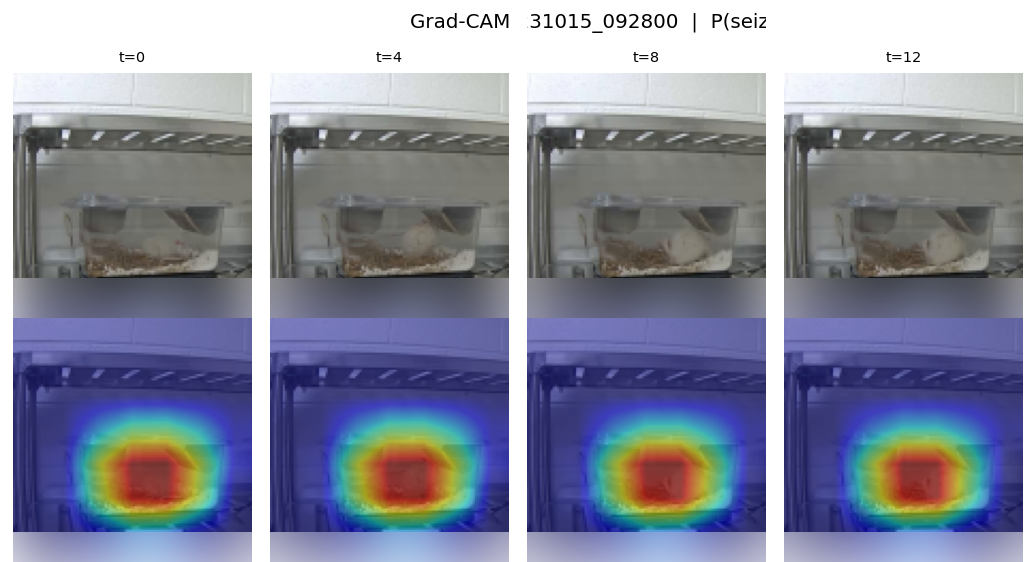
\includegraphics[width=\linewidth, trim=0 0 0 42, clip]{fig/gradcam_stage4_deid_4f.png}\\[1pt]
{\footnotesize (a) Seizure clip (Stage\,4): activation concentrates on the animal}\\[4pt]
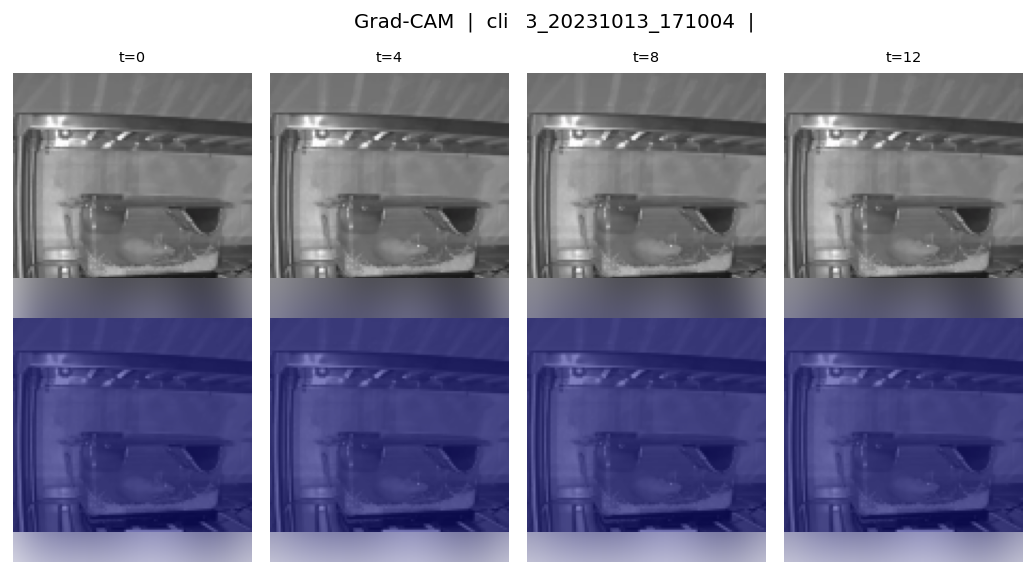
\includegraphics[width=\linewidth, trim=0 0 0 42, clip]{fig/gradcam_nonseizure_deid_4f.png}\\[1pt]
{\footnotesize (b) Non-seizure clip: activation is diffuse, with no focus on the animal}
\caption{Grad-CAM~\cite{selvaraju2017gradcam} for the R(2+1)D detector; each strip
shows input frames (top) and seizure-class activation (bottom), for four of the
eight sampled frames. \emph{(a)}~On a Stage\,4 clip, activation concentrates on the
animal during convulsive motion. \emph{(b)}~On a non-seizure clip it stays diffuse.
The contrast indicates the detector responds to behavior rather than cage
background. All eight frames at full width are in App.~\ref{sec:qualitative:gradcam},
Fig.~\ref{fig:gradcamfull}. De-identified clips; identifier bands redacted.}
\label{fig:gradcam}
\end{figure}



\begin{takeaway}
\takeawaylabel Detection is limited by temporal context rather than by model size. Ten backbones
spanning every paradigm land within 0.03 macro-F1 and a 4M-parameter model ties a 33M
one, while a single frame collapses to 0.569. Sixteen to thirty-two frames at
$112$\,px suffices, and the shortcut controls available to us are consistent with a
behavioral detector without settling the question.
\end{takeaway}

\subsection{Cross-modal comparison, generalization and external validation}
\label{sec:crossmodal}

With the capacity question settled, we turn to how far the video result carries: how
it stands against an electrode-based reference, whether it survives held-out animals
and harder label granularities, and whether it reproduces on a public benchmark.

\noindent\textbf{Is the EEG baseline strong enough?}
Because the headline is a cross-modal comparison, the EEG side must be a strong
baseline. Each EEG model consumes the first recorded EEG channel decimated to
125\,Hz, cut into 6\,s windows at 3\,s stride and z-scored per window; a clip
decision is the log-mean of the per-window posteriors (App.~\ref{sec:eegsweep}). On these identical windows,
split and seed we evaluate seven EEG models (Table~\ref{tab:eegarch}), chosen to
span how the temporal structure of a trace can be modeled. Five are deep. The GRU above and an LSTM~\cite{hochreiter1997lstm} read the window as a raw sequence. EEGNet~\cite{lawhern2018eegnet} is a compact CNN whose first layer acts as a learned bandpass filter bank, the EEG Conformer~\cite{song2022conformer} puts a self-attention encoder over convolutional tokens, and a dilated temporal convolutional network (TCN)~\cite{bai2018tcn} grows its receptive field exponentially with depth. Two are classical: Random Forest~\cite{breiman2001rf} and
XGBoost~\cite{chen2016xgboost} learn no representation and instead consume a fixed
per-window descriptor of band powers and time-domain statistics. The strongest at detection is the TCN, at 0.978\,$\pm$\,0.001 macro-F1 and 0.996
AUROC, a little above the GRU (0.974\,$\pm$\,0.003); it also leads at 3-class
(0.767 \vs\ 0.750). At 5-class the two are tied within seed noise
(0.563\,$\pm$\,0.012 \vs\ 0.560\,$\pm$\,0.005), so the ordering that holds
across the table is TCN\,$\geq$\,GRU\,$>$\,Conformer\,$>$\,LSTM\,$>$\,EEGNet
rather than a single winner. The spread across the five deep models is
0.055 macro-F1 at detection but 0.147 at 3-class and 0.154 at 5-class: architecture
is close to irrelevant for detecting a seizure and matters considerably for grading
one, the mirror image of the backbone-agnostic result on the video side
(Table~\ref{tab:vidarch}). The classical baselines are competitive at detection,
where feature-based XGBoost reaches 0.914 against the deep EEGNet's 0.923, but fall
away at grading (0.466 \vs\ 0.563 for the TCN at 5-class), so the deep advantage on
EEG is small where the task is easy and real where it is hard. The LSTM is the least
reliable model in the field: two of its fifteen runs failed to converge outright,
which no other backbone did. One caveat bounds the absolute margin: this EEG
reference is single-channel, so a richer montage could narrow the reported
cross-modal gap.

Architecture diversity is not tuning, so we also sweep the EEG side's window,
stride, sampling rate and clip-pooling rule, and every model in
Table~\ref{tab:eegarch} is trained at the winning setting
(App.~\ref{sec:eegsweep}). The sweep is informative about which axis matters.
Window length is nearly flat---2, 4, 6 and 8\,s span 0.015 macro-F1, less than the
0.018 range we measure across seeds at a fixed setting---while stride is monotone
(0.554 at 1.5\,s to 0.496 at 6\,s) and sampling rate is the largest single effect
(dropping to 62.5\,Hz costs 0.049). The clip-pooling rule, an axis rarely swept at
all, is worth more than any of them: log-mean beats the usual mean on seven of eight
configurations and gains 0.028 macro-F1 at the winning setting, for free, since it
re-scores stored window posteriors without retraining. Because pooling and window
interact---the best window under mean pooling is only fourth-best under
log-mean---we select the best \emph{pair} rather than optimizing the axes in
sequence. Even so, the tuned EEG reference does not close the cross-modal gap: the
strongest EEG model at 5-class reaches 0.563 against video's 0.657.

\noindent\textbf{Does the ordering depend on the metric?}
Macro-F1 and MCC weight the confusion matrix differently, so we report both
throughout (Sec.~\ref{sec:problem}). They disagree about how hard grading \emph{looks}: at 5-class video scores 0.657 macro-F1 against 0.831 MCC. They agree on every ordering that carries a claim. The cross-modal gap widens with granularity under both, and the ten backbones stay clustered under both. The headline conclusions are therefore a property of the data, not of the summary statistic; App.~\ref{sec:metrics} works this through.

\begin{table*}[t]
\centering
\caption{EEG backbone comparison (identical windows and split) across all three
granularities, as mean\,$\pm$\,std over five seeds. Precision/recall/F1 are
macro-averaged; detection AUROC is binary, grading AUROC macro one-vs-rest; MCC is the
multiclass Matthews correlation coefficient. All models use the configuration selected
in App.~\ref{sec:eegsweep}: 6\,s windows at 3\,s stride, 125\,Hz, logmean clip
pooling. The TCN leads at detection and 3-class; at 5-class it and the GRU are tied
within noise (0.563\,$\pm$\,0.012 \vs\ 0.560\,$\pm$\,0.005). Random Forest and
XGBoost use per-window band-power and time-domain features; XGBoost is deterministic
given the data, hence $\pm$0.000. Two of fifteen LSTM runs failed to converge
(macro-F1 0.231 and 0.136 against cell medians of 0.677 and 0.456); they are excluded
from the LSTM means, which therefore rest on $n{=}3$ at 3-class and $n{=}4$ at 5-class.
Best per column \textbf{bold}, second-best \underline{underlined}.}
\label{tab:eegarch}
\setlength{\tabcolsep}{3pt}
\renewcommand{\arraystretch}{1.15}
\resizebox{\textwidth}{!}{%
\begin{tabular}{@{}l ccccc ccccc ccccc@{}}
\toprule
 & \multicolumn{5}{c}{\textbf{Detection (2-class)}} & \multicolumn{5}{c}{\textbf{3-class}} & \multicolumn{5}{c}{\textbf{5-class}} \\
\cmidrule(lr){2-6}\cmidrule(lr){7-11}\cmidrule(lr){12-16}
\textbf{EEG backbone} & \textbf{P} & \textbf{R} & \textbf{F1} & \textbf{AUC} & \textbf{MCC} & \textbf{P} & \textbf{R} & \textbf{F1} & \textbf{AUC} & \textbf{MCC} & \textbf{P} & \textbf{R} & \textbf{F1} & \textbf{AUC} & \textbf{MCC} \\
\midrule
\multicolumn{16}{@{}l}{\itshape Deep}\\
GRU~\cite{ganguly2025} & \underline{0.975}\,{\scriptsize$\pm$0.003} & \underline{0.974}\,{\scriptsize$\pm$0.003} & \underline{0.974}\,{\scriptsize$\pm$0.003} & \underline{0.996}\,{\scriptsize$\pm$0.001} & \underline{0.949}\,{\scriptsize$\pm$0.005} & \underline{0.744}\,{\scriptsize$\pm$0.014} & 0.764\,{\scriptsize$\pm$0.013} & \underline{0.750}\,{\scriptsize$\pm$0.010} & \underline{0.956}\,{\scriptsize$\pm$0.002} & \underline{0.823}\,{\scriptsize$\pm$0.014} & \textbf{0.556}\,{\scriptsize$\pm$0.040} & \underline{0.635}\,{\scriptsize$\pm$0.035} & \underline{0.560}\,{\scriptsize$\pm$0.005} & \textbf{0.941}\,{\scriptsize$\pm$0.003} & \textbf{0.728}\,{\scriptsize$\pm$0.032} \\
LSTM~\cite{hochreiter1997lstm} & 0.972\,{\scriptsize$\pm$0.008} & 0.971\,{\scriptsize$\pm$0.007} & 0.971\,{\scriptsize$\pm$0.008} & 0.994\,{\scriptsize$\pm$0.004} & 0.942\,{\scriptsize$\pm$0.015} & 0.696\,{\scriptsize$\pm$0.041} & 0.741\,{\scriptsize$\pm$0.067} & 0.698\,{\scriptsize$\pm$0.053} & 0.937\,{\scriptsize$\pm$0.027} & 0.743\,{\scriptsize$\pm$0.059} & 0.476\,{\scriptsize$\pm$0.042} & 0.555\,{\scriptsize$\pm$0.100} & 0.468\,{\scriptsize$\pm$0.052} & 0.903\,{\scriptsize$\pm$0.039} & 0.598\,{\scriptsize$\pm$0.059} \\
EEGNet~\cite{lawhern2018eegnet} & 0.926\,{\scriptsize$\pm$0.011} & 0.922\,{\scriptsize$\pm$0.013} & 0.923\,{\scriptsize$\pm$0.012} & 0.975\,{\scriptsize$\pm$0.005} & 0.848\,{\scriptsize$\pm$0.023} & 0.646\,{\scriptsize$\pm$0.010} & 0.676\,{\scriptsize$\pm$0.018} & 0.620\,{\scriptsize$\pm$0.015} & 0.903\,{\scriptsize$\pm$0.005} & 0.626\,{\scriptsize$\pm$0.031} & 0.448\,{\scriptsize$\pm$0.040} & 0.488\,{\scriptsize$\pm$0.025} & 0.409\,{\scriptsize$\pm$0.039} & 0.864\,{\scriptsize$\pm$0.011} & 0.499\,{\scriptsize$\pm$0.037} \\
EEG Conformer~\cite{song2022conformer} & 0.972\,{\scriptsize$\pm$0.001} & 0.972\,{\scriptsize$\pm$0.001} & 0.972\,{\scriptsize$\pm$0.001} & 0.988\,{\scriptsize$\pm$0.002} & 0.943\,{\scriptsize$\pm$0.001} & 0.719\,{\scriptsize$\pm$0.009} & \underline{0.784}\,{\scriptsize$\pm$0.013} & 0.729\,{\scriptsize$\pm$0.010} & 0.952\,{\scriptsize$\pm$0.002} & 0.780\,{\scriptsize$\pm$0.017} & 0.512\,{\scriptsize$\pm$0.004} & 0.624\,{\scriptsize$\pm$0.032} & 0.523\,{\scriptsize$\pm$0.005} & 0.936\,{\scriptsize$\pm$0.008} & 0.683\,{\scriptsize$\pm$0.008} \\
TCN~\cite{bai2018tcn} & \textbf{0.979}\,{\scriptsize$\pm$0.001} & \textbf{0.978}\,{\scriptsize$\pm$0.001} & \textbf{0.978}\,{\scriptsize$\pm$0.001} & \textbf{0.996}\,{\scriptsize$\pm$0.001} & \textbf{0.957}\,{\scriptsize$\pm$0.002} & \textbf{0.758}\,{\scriptsize$\pm$0.014} & \textbf{0.786}\,{\scriptsize$\pm$0.008} & \textbf{0.767}\,{\scriptsize$\pm$0.007} & \textbf{0.960}\,{\scriptsize$\pm$0.001} & \textbf{0.839}\,{\scriptsize$\pm$0.015} & \underline{0.537}\,{\scriptsize$\pm$0.008} & \textbf{0.654}\,{\scriptsize$\pm$0.013} & \textbf{0.563}\,{\scriptsize$\pm$0.012} & \underline{0.941}\,{\scriptsize$\pm$0.003} & \underline{0.728}\,{\scriptsize$\pm$0.021} \\
\midrule
\multicolumn{16}{@{}l}{\itshape Classical (band-power $+$ statistical features)}\\
Random Forest~\cite{breiman2001rf} & 0.885\,{\scriptsize$\pm$0.001} & 0.852\,{\scriptsize$\pm$0.001} & 0.852\,{\scriptsize$\pm$0.001} & 0.986\,{\scriptsize$\pm$0.000} & 0.737\,{\scriptsize$\pm$0.002} & 0.541\,{\scriptsize$\pm$0.001} & 0.542\,{\scriptsize$\pm$0.001} & 0.529\,{\scriptsize$\pm$0.001} & 0.934\,{\scriptsize$\pm$0.001} & 0.613\,{\scriptsize$\pm$0.002} & 0.477\,{\scriptsize$\pm$0.001} & 0.328\,{\scriptsize$\pm$0.001} & 0.332\,{\scriptsize$\pm$0.002} & 0.916\,{\scriptsize$\pm$0.002} & 0.503\,{\scriptsize$\pm$0.002} \\
XGBoost~\cite{chen2016xgboost} & 0.922\,{\scriptsize$\pm$0.000} & 0.913\,{\scriptsize$\pm$0.000} & 0.914\,{\scriptsize$\pm$0.000} & 0.984\,{\scriptsize$\pm$0.000} & 0.835\,{\scriptsize$\pm$0.000} & 0.657\,{\scriptsize$\pm$0.000} & 0.684\,{\scriptsize$\pm$0.000} & 0.642\,{\scriptsize$\pm$0.000} & 0.934\,{\scriptsize$\pm$0.000} & 0.623\,{\scriptsize$\pm$0.000} & 0.479\,{\scriptsize$\pm$0.000} & 0.530\,{\scriptsize$\pm$0.000} & 0.466\,{\scriptsize$\pm$0.000} & 0.924\,{\scriptsize$\pm$0.000} & 0.529\,{\scriptsize$\pm$0.000} \\
\bottomrule
\end{tabular}}
\end{table*}

\noindent\textbf{Generalization to unseen subjects.}
Session-disjoint validation still trains and tests on the \emph{same} animals. The
stricter, deployment-relevant question is whether the detector transfers to an animal it has never seen, the protocol RodEpil~\cite{rodepil2025} adopts. We
therefore repeat all three tasks under \emph{subject-disjoint} five-fold
cross-validation, holding out four whole animals per fold
(Table~\ref{tab:subjectwise}). At detection, neither modality is much troubled by the
harder protocol. Video degrades only marginally, from 0.968 to 0.948 macro-F1 and 0.993 to 0.985 AUROC. The EEG GRU is essentially unchanged, moving from 0.974 to 0.972, and the two fold spreads are nearly identical ($\sigma$ 0.016 against 0.019). The two are therefore equally stable across held-out animals, and EEG ends up marginally ahead. That reverses the session-disjoint ordering, though both differences are small relative to the fold spread (Fig.~\ref{fig:stability}). Detection generalizes across animals in both
modalities; the modalities separate at grading, not here. Part of the residual
cross-subject difficulty is visual: cage framing, lighting, and coat vary from
animal to animal (App.~\ref{sec:dataextra:crosssubj}, Fig.~\ref{fig:crosssubj}).

Grading is where the protocol bites. Holding out whole animals costs video 0.060
macro-F1 at 3-class and 0.182 at 5-class (0.780\,$\to$\,0.720 and
0.657\,$\to$\,0.475), against 0.094 and 0.156 for the EEG reference, so the cross-modal margin at 5-class narrows from 0.097 to 0.071. Video still leads at both grading granularities: 0.720 against 0.656 at 3-class, and 0.475 against 0.404 at 5-class. The two now degrade at comparable rates, and video is no longer uniformly the steadier across folds.
We read the larger video drop as the price of appearance: a held-out animal arrives
with unfamiliar cage framing, lighting and coat, and at five classes the model must
separate stages that differ by subtle motion on top of that shift. Fine-grained
grading across unseen animals is thus the weakest regime we measure for either
modality, and the accurate statement of our result is that video's advantage is
largest within a cohort and narrower, though still substantial, across new animals.

% fig:crosssubj now lives in the supplement (App. C, sec:dataextra:crosssubj).


\begin{figure}[t]
\centering
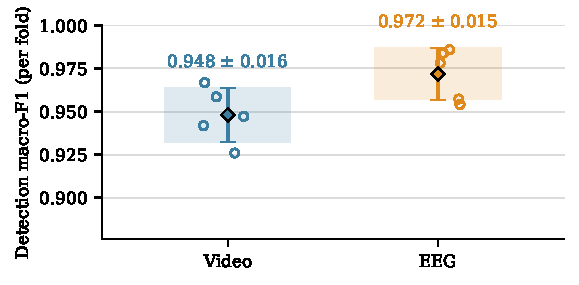
\includegraphics[width=\linewidth]{fig/fig_stability.pdf}
\caption{Cross-subject stability under subject-disjoint 5-fold CV (per-fold
detection macro-F1 from Table~\ref{tab:subjectwise}; dots are folds, diamonds are
the mean, whiskers/bands are $\pm1\sigma$). Both modalities are tightly and comparably clustered, video at $0.948\pm0.016$ over $[0.926,0.967]$ and EEG at $0.972\pm0.015$ over $[0.954,0.986]$, so detection transfers to unseen animals about equally well either way, with EEG marginally ahead on the mean. The
modalities diverge at grading instead (Table~\ref{tab:subjectwise}).}
\label{fig:stability}
\end{figure}

\begin{table}[tb]
\centering
\caption{Generalization from session-disjoint to subject-disjoint (5-fold, whole animals
held out) at all three granularities. The protocols separate the two regimes cleanly.
At detection, holding out whole animals costs video 0.022 macro-F1 and costs the EEG reference nothing (0.974\,$\to$\,0.972), so EEG is ahead on unseen animals and the two
are equally stable across folds ($\pm$0.015 \vs\ $\pm$0.016; MCC $\pm$0.030 \vs\
$\pm$0.031). At grading video leads under both protocols, though it gives up more when animals are held out, 0.187 macro-F1 at 5-class against 0.159 for EEG, so the margin narrows from 0.128 to 0.100. Subject-disjoint entries are mean\,$\pm$\,std over folds.}
\label{tab:subjectwise}
\setlength{\tabcolsep}{3pt}
\renewcommand{\arraystretch}{1.2}
\resizebox{\columnwidth}{!}{%
\begin{tabular}{@{}l l cc ccc@{}}
\toprule
 & & \multicolumn{2}{c}{\textbf{Session-dis.}} & \multicolumn{3}{c}{\textbf{Subject-disjoint (5-fold)}} \\
\cmidrule(lr){3-4}\cmidrule(lr){5-7}
\textbf{Task} & \textbf{Mod.} & \textbf{Macro-F1} & \textbf{MCC} & \textbf{Macro-F1} & \textbf{AUROC} & \textbf{MCC} \\
\midrule
\multirow{2}{*}{Detection} & Video & 0.968 & 0.936 & 0.948\,{\scriptsize$\pm$0.016} & 0.985\,{\scriptsize$\pm$0.006} & 0.896\,{\scriptsize$\pm$0.031} \\
                           & EEG   & \textbf{0.974} & \textbf{0.949} & \textbf{0.972}\,{\scriptsize$\pm$0.015} & \textbf{0.995}\,{\scriptsize$\pm$0.005} & \textbf{0.944}\,{\scriptsize$\pm$0.030} \\
\midrule
\multirow{2}{*}{3-class}   & Video & \textbf{0.780} & \textbf{0.853} & \textbf{0.720}\,{\scriptsize$\pm$0.028} & \textbf{0.942}\,{\scriptsize$\pm$0.015} & 0.761\,{\scriptsize$\pm$0.029} \\
                           & EEG   & 0.750 & 0.823 & 0.656\,{\scriptsize$\pm$0.022} & 0.916\,{\scriptsize$\pm$0.025} & \textbf{0.793}\,{\scriptsize$\pm$0.046} \\
\midrule
\multirow{2}{*}{5-class}   & Video & \textbf{0.657} & \textbf{0.831} & \textbf{0.475}\,{\scriptsize$\pm$0.024} & \textbf{0.888}\,{\scriptsize$\pm$0.026} & \textbf{0.676}\,{\scriptsize$\pm$0.041} \\
                           & EEG   & 0.560 & 0.728 & 0.404\,{\scriptsize$\pm$0.042} & 0.831\,{\scriptsize$\pm$0.076} & 0.657\,{\scriptsize$\pm$0.107} \\
\bottomrule
\end{tabular}}
\end{table}

\noindent\textbf{Grading: video degrades, EEG collapses.}
Severity is harder, and here the two modalities part ways. As the task moves from
2-class detection to 3-class (non-seizure / mild / severe) and 5-class
(non-seizure / Stage\,2--5) grading, video macro-F1 declines gracefully from
0.968 to 0.780 to 0.657 and stays usable even at five levels. Even the rare severe
classes retain a workable signal (Stage\,5 per-class F1 0.42 at 5-class;
App.~\ref{sec:extraresults:ablations}, Table~\ref{tab:perclass}). The EEG reference
declines more steeply from the same starting point
(0.974\,$\to$\,0.750\,$\to$\,0.560), and its rarest classes are where it gives way
(Stage\,4 F1 0.20, Stage\,5 F1 0.12 against 0.36 and above for video; the per-class
breakdown is given in Table~\ref{tab:perclass} and Figure~\ref{fig:perclassbar}).
Video thus retains a workable severity signal where EEG does not, though
fine-grained grading remains the weakest regime for both. The hardest cases are
rare mild events and data-poor animals (App.~\ref{sec:qualitative:failures},
Fig.~\ref{fig:hardcases}). Figure~\ref{fig:degrade} traces the two
curves side by side: they start level but the video line stays high while the EEG
line dives, the gap widening from 0.004 at detection to 0.128 at 5-class.

\noindent\textbf{Do the two modalities fail the same way?}
An aggregate gap says which model is better, not whether the other is redundant, so
we compare the errors themselves (App.~\ref{sec:extraresults:failure},
Fig.~\ref{fig:confusion}). They differ in kind. Video's mistakes are ordinal
near-misses: $72.4\%$ land on an adjacent stage, and the largest single cell is
Stage\,4 read as Stage\,3 ($95$ of $167$ clips). It registers that a convulsion is
underway and misjudges the degree. The EEG reference adds two failure modes video
does not have. It loses events outright, calling $10.1\%$ of Stage\,3 clips non-seizure against $2.3\%$ for video, and its errors ignore the ordinal scale,
$44\%$ landing two or more stages away against $28\%$ for video (mean
$|\Delta\text{stage}|$ $1.51$ \vs\ $1.30$). A single channel supports a
seizure/no-seizure decision without carrying a monotone severity axis. The one
exception is the informative one: at Stage\,2, the rung with the least whole-body
movement, the ordering reverses and EEG recalls $0.863$ against video's $0.650$.
Video's advantage is behavioral, and it recedes exactly where the behavior does.
Across the clips both models scored, video alone is correct on $14.2\%$ and EEG
alone on $4.9\%$ (Table~\ref{tab:paired}), so each modality recovers clips the other
loses. That is a measured case for the fusion we leave to future work
(Sec.~\ref{sec:open}).

% fig:hardcases now lives in the supplement (App. D, sec:qualitative:failures).

\begin{figure}[t]
\centering
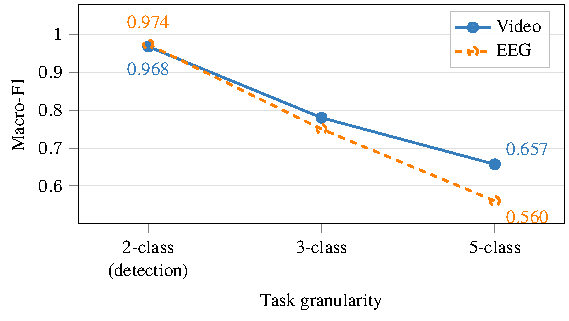
\includegraphics[width=\linewidth]{fig/fig_degrade.pdf}
\caption{Video degrades more gracefully than EEG as the task hardens (macro-F1,
values from Table~\ref{tab:results}). The two modalities are level at detection
(0.968 \vs\ 0.974), and by 5-class grading video still retains a usable 0.657
whereas the EEG GRU falls to 0.560, so a 0.006 EEG lead at detection becomes a 0.097 video lead at five classes.}
\label{fig:degrade}
\end{figure}

\noindent\textbf{External validation on RodEpil.}
To test whether these detection numbers transfer beyond our own cohort, we
evaluate the same R(2+1)D backbone on the public RodEpil
benchmark~\cite{rodepil2025} (13{,}053 clips, 19 rats) under its native
\emph{subject-wise} five-fold protocol. A direct run scores a suspicious 0.9996
F1, because the raw release leaks the class label into low-level clip encoding.
Every normal clip is stored at 30\,fps / 301 frames and every seizure clip at
29\,fps / 291 frames. Either attribute alone separates the classes with AUROC 1.0, and the per-clip crop resolution also differs by class. Re-encoding
all clips through a single uniform pipeline ($224\times224$ letterbox, 30\,fps,
300 frames, identical codec) removes this shortcut, and the backbone then reaches
\textbf{0.979 subject-wise F1} (AUROC 0.999; per-fold in Table~\ref{tab:rodepil}).
This matches the dataset's TimeSformer baseline (0.97) and reflects genuine
behavior: the per-fold learning curve now rises gradually instead of saturating
at epoch one. We flag the encoding confound as a caution for future users of this
otherwise valuable benchmark.

\begin{table}[tb]
\centering
\caption{External validation on RodEpil~\cite{rodepil2025} (subject-wise 5-fold,
seizure-class F1 and MCC). The raw release is separable by an encoding artifact that
inflates detection to near-perfect; re-encoding every clip through one uniform
pipeline removes the shortcut and yields honest scores on par with the dataset's
TimeSformer baseline (0.97).}
\label{tab:rodepil}
\setlength{\tabcolsep}{5pt}
\renewcommand{\arraystretch}{1.15}
\resizebox{\columnwidth}{!}{%
\begin{tabular}{@{}l ccccc c@{}}
\toprule
 & \textbf{F0} & \textbf{F1} & \textbf{F2} & \textbf{F3} & \textbf{F4} & \textbf{Mean} \\
\midrule
Raw (leaked) F1  & 1.000 & 0.998 & 1.000 & 1.000 & 1.000 & \textbf{0.9996} \\
Raw (leaked) MCC & 1.000 & 0.998 & 1.000 & 1.000 & 1.000 & \textbf{0.9995} \\
\midrule
Re-encoded F1    & 0.965 & 0.978 & 0.997 & 0.977 & 0.979 & \textbf{0.979} \\
Re-encoded AUROC & 0.999 & 1.000 & 1.000 & 1.000 & 0.998 & \textbf{0.999} \\
Re-encoded MCC   & 0.957 & 0.976 & 0.996 & 0.967 & 0.964 & \textbf{0.972} \\
\bottomrule
\end{tabular}}
\end{table}

\noindent\textbf{All backbones on RodEpil.}
Running the full ten-backbone suite on re-encoded RodEpil reshuffles the ranking and widens it, from a 0.03 band on our own cohort to 0.87--0.99 macro-F1. The convolutional networks lead and the attention models trail, the reverse of our ordering. Backbone choice is therefore a data-regime effect, not a universal ranking (App.~\ref{sec:extraresults}, Table~\ref{tab:rodepilbb}).

\begin{figure}[t]
\centering
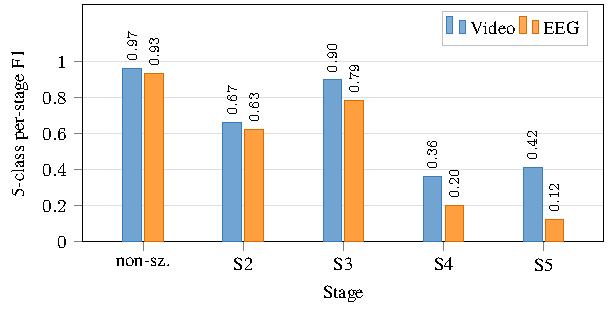
\includegraphics[width=\linewidth]{fig/fig_perclassbar.pdf}
\caption{Per-stage F1 at the hardest 5-class grading task
(Table~\ref{tab:perclass}). Both modalities are strong on the common classes, non-seizure and Stage\,3. On the rare severe stages EEG gives way, with S4/S5 F1 of 0.20 and 0.12, while video retains a usable signal at 0.36 and 0.42. Video holds a workable severity cue where the electrode-based model gives out.}
\label{fig:perclassbar}
\end{figure}



\begin{takeaway}
\takeawaylabel Video matches the EEG reference at detection (0.968 against 0.974)
and pulls ahead as the task becomes behavioral, reaching 0.657 against 0.560 at five-class. That ordering survives both held-out animals and the public RodEpil benchmark, though the margin is widest within a cohort and narrows once whole animals are held out. The two also fail differently: video misgrades by one stage, EEG loses events and scatters across non-adjacent ones, and at Stage\,2 the ordering reverses. Their errors are complementary.
\end{takeaway}

\subsection{Does inverse-frequency weighting keep the long tail from
dominating the result?}
\label{sec:rq3}

Two independent imbalances run through this cohort, and both threaten to turn a
pooled score into a report on the majority. The first is across stages: the
five-class validation set is $51\%$ non-seizure and $41\%$ Stage\,3, while Stage\,5
is 34 clips, a ratio of $80{:}1$ between the largest and smallest class. The second
is across animals, whose totals span 11 to 3{,}091 clips
(App.~\ref{sec:dataextra:cohort}). A model that ignored every rare stage and every
quiet animal could still look strong on aggregate accuracy.

\noindent\textbf{Three defenses, at construction, objective and measurement.}
Detection sidesteps the problem by construction: each seizure clip is paired with a
matched negative, so the binary task is near-balanced ($12{,}197$ against
$11{,}934$) and imbalance enters only at grading. At grading the objective carries
it: we train with inverse-frequency-weighted cross-entropy, weights normalized to
mean one, which at five-class gives Stage\,5 roughly $60\times$ the weight of
non-seizure. Measurement then keeps the tail visible. Every score is macro-averaged, every pooled number is paired with a per-subject breakdown, and the generalization study holds out whole animals (Table~\ref{tab:subjectwise}). A model that quietly abandons the tail cannot hide behind a pooled figure. One caveat applies to the metrics themselves. AUROC is optimistic under strong imbalance~\cite{saito2015prc}, which is why macro-F1 carries the argument at the rare stages.

\noindent\textbf{The tail stays learnable.}
The defenses work in the sense that matters first: the rare stages are predicted
rather than weighted out of existence. A majority-class predictor reaches only
0.136 macro-F1 at five-class, against the video model's 0.657, and the model still
recovers a third of the Stage\,5 clips (recall 0.324 on 34 examples) at 0.579
precision (Table~\ref{tab:perclass}).

\noindent\textbf{What it costs.}
Re-weighting redistributes error rather than removing it, and two limits follow.
The tail remains the weakest regime: Stage\,4 and Stage\,5 F1, 0.362 and 0.415, sit far below Stage\,3 at 0.900. The correction mitigates imbalance without solving it. More
instructive is what happens when the same correction meets a weaker signal. The EEG
model's Stage\,5 precision is 0.014 against recall 0.121: it assigns Stage\,5 to
roughly nine times as many clips as actually carry it, converting a rare-class blind
spot into a false-positive one. Up-weighting a class the modality cannot separate buys recall at a price in precision that a screening tool would not accept. The imbalance strategy should therefore be chosen per modality, not globally.

One caveat bounds all of this. We report the behavior of a single reasonable strategy: inverse-frequency weighting is never compared against unweighted training, resampling~\cite{chawla2002smote} or a focal objective~\cite{lin2017focal}, three standard options surveyed in~\cite{johnson2019imbalance} (Sec.~\ref{sec:open}).

\begin{takeaway}
\takeawaylabel Weighting keeps the tail learnable rather than solving it. Rare stages are
predicted instead of collapsing to the majority (0.657 macro-F1 against 0.136 for a
majority-class predictor, with Stage\,5 recall 0.324 on 34 clips), yet they remain
the weakest regime, and on the weaker modality the same correction over-predicts
Stage\,5 roughly ninefold.
\end{takeaway}

\subsection{Why behavioral video matters}
\label{sec:discussion}

Taken together, the results show a camera matching electrodes at detection under
both protocols and pulling ahead once the endpoint is itself behavioral. Three
consequences follow.

\noindent\textbf{Video reads the endpoint directly.}
The Racine scale grades motor manifestations: twitching, rearing, forelimb clonus,
falling~\cite{racine1972}. A camera observes the signal the grade is defined on,
while an electrode observes a correlate of it. That is the simplest account of
Fig.~\ref{fig:degrade}. The modalities are indistinguishable while the question is
whether an event occurred, and separate once it becomes how severe that event was,
with the largest gap at the rarest and most severe stage (Stage\,5 per-class F1
0.42 against 0.12).

\noindent\textbf{Cost, scale and welfare favor the camera.}
Electrode EEG needs surgical implantation, which is expensive, low-throughput, and a
source of infection, signal drift and welfare burden. A camera is cheap,
surgery-free, and watches many cages at once, so video-only screening scales to the
cohorts preclinical drug discovery needs and reduces harm in the spirit of the 3Rs.
Deployment is equally favorable: the 4M-parameter X3D-M matches the 33M R(2+1)D
(Table~\ref{tab:vidspec}), which puts continuous monitoring on modest hardware
within reach.

\noindent\textbf{Electrodes remain necessary, and fusion is the next step.}
Our EEG reference is a single channel, and its limits show throughout: it loses
$10.1\%$ of Stage\,3 events outright, carries no monotone severity axis, and
supplies no localization. A richer montage would ease all three. Even so, EEG
captures electrographic-only seizures that have no motor correlate at all, recovers
onset timing, and recovers the Stage\,2 events video misses
(Sec.~\ref{sec:crossmodal}); a camera is blind to each of these. Video does not
displace the electrode; it carries the behavioral half of the workflow, which is the
half that consumes expert time. We keep the two streams unfused here deliberately.
A fused model would confound the question we set out to answer, namely how far each modality gets on its own. No shared paired video--EEG benchmark yet exists on which such a model could be compared against prior work (Sec.~\ref{sec:open}).

\begin{takeaway}
\takeawaylabel A camera alone matches electrode-based detection, on held-out
sessions and held-out animals alike, and grades severity more accurately.
Electrodes stay necessary for electrographic-only events, onset timing, and the
mildest behavioral stage.
\end{takeaway}


\section{Limitations and Future Work}
\label{sec:open}

Our study is deliberately scoped to unimodal models on one preclinical cohort, and
five limitations follow from that scope. Generalization rests on five
subject-disjoint folds of a single cohort, so multi-cohort, subject-wise evaluation
remains the honest test, and fine-grained severity on unseen animals is where video
gives up the most (0.662 to $0.475$ macro-F1, Table~\ref{tab:subjectwise}). Severity
grading is the open task: the rare severe stages carry most of the error and invite
targeted collection or the ordinal formulation of Sec.~\ref{sec:problem:ordinal},
and our inverse-frequency weighting is reported without an ablation against
resampling~\cite{chawla2002smote} or a focal objective~\cite{lin2017focal}.
Cross-modal artifact rejection---the original clinical reason for recording both
streams---remains almost unexploited computationally~\cite{frontiers_fusion2026},
and no public \emph{paired} video--EEG animal benchmark exists to test it
on~\cite{rodepil2025}. Finally, monitoring that runs for weeks makes streaming,
on-device inference a practical prerequisite~\cite{vepinet2024}.
App.~\ref{sec:openfull} develops each of the five in full.

\section{Conclusion}
\label{sec:conclusion}

We presented a large-scale empirical study of video and EEG deep learning
for automated rodent seizure detection and severity grading, built on a pooled
twenty-subject synchronized cohort of $\sim$24k clips. Under a single controlled,
leakage-aware protocol, and across ten video backbones and seven EEG models, four
results stand out: a standard Kinetics-pretrained R(2+1)D backbone \emph{matches}
a strong EEG reference for seizure \emph{detection} (0.993 \vs\ 0.992 AUROC) from
a non-invasive camera alone; detection is essentially backbone-agnostic, so a 4M
model ties a 33M one; video \emph{degrades more gracefully than EEG on severity
grading}, the one regime where the two clearly separate; and Grad-CAM confirms
the detector attends to genuine behavior. The same backbone reaches 0.979 F1 on
the public RodEpil benchmark once a raw-release encoding artifact is corrected.
Together these findings show that the behavioral half of the video--EEG gold
standard is far more automatable than its scarce use in animal studies suggests.
The natural next step is principled, artifact-aware \emph{fusion} of the two
modalities---validated on shared benchmarks and evaluated across subjects---for
which this study provides both the motivation and the single-modality baselines.


{
    \small
    \bibliographystyle{ieeenat_fullname}
    \bibliography{main}
}

% ---------------------------------------------------------------------------
% Supplementary material: the full literature survey (video / video-EEG
% seizure detection across modality x subject). Kept out of the main empirical
% paper; for a WACV submission this can be split into a separate PDF.
% ---------------------------------------------------------------------------
\clearpage
\appendix
\section{Supplementary: A Survey of Video and Video--EEG Seizure Detection}
\label{sec:survey}

This appendix provides the comprehensive literature survey that motivates the
empirical study in the main paper. We organize prior work along two axes, modality (EEG-only, video-only, fused video--EEG) and subject (human \vs\ animal), and review the video-understanding backbones that make behavioral
read-out tractable. The main-paper Related Work (Sec.~\ref{sec:related}) is a
condensed positioning drawn from this material.

\subsection{Scope and Taxonomy}
\label{sec:taxonomy}

This subsection fixes the scope of the survey and of the positioning in
Sec.~\ref{sec:related}. We restrict attention to \emph{automated} seizure
detection (methods that
consume raw or lightly processed EEG, video, or both, and output a
seizure/non-seizure label or a severity grade) and organize it along two axes.

\noindent\textbf{Axis 1: modality.}
(i)~\emph{EEG-only} methods dominate historically and clinically. They range from
hand-crafted spectral features fed to classical classifiers to end-to-end
recurrent and convolutional networks. (ii)~\emph{Video-only} methods read behavior
directly through pose estimation or action recognition, and their non-invasiveness
makes them attractive. (iii)~\emph{Fused video--EEG} methods combine both streams
and, in principle, inherit the strengths of each.

\noindent\textbf{Axis 2: subject.}
Human clinical epilepsy monitoring units generate the largest annotated corpora
and host most multimodal work. \emph{Animal} (rodent, canine, porcine) models
drive preclinical drug discovery, yet automated multimodal methods there remain
scarce.

Table~\ref{tab:gap} previews where the field is mature and where it is open. The
EEG-only cells are crowded. The video-only cells are filling in for humans and now
emerging for animals, with a first public rodent benchmark appearing in
2025~\cite{rodepil2025}. The fused video--EEG animal cell remains nearly
empty: the gap that motivates our empirical study.

\begin{table}[t]
\centering
\caption{Research gap analysis. Rows are ordered from mature (top) to open
(bottom). The fused video--EEG animal setting is barely populated.}
\label{tab:gap}
\setlength{\tabcolsep}{4pt}
\renewcommand{\arraystretch}{1.2}
\begin{tabular}{@{}p{2.5cm} p{2.6cm} p{2.4cm}@{}}
\toprule
\textbf{Setting} & \textbf{State of the art} & \textbf{Gap} \\
\midrule
EEG-only, animal & GRU/LSTM, DCNN~\cite{ganguly2025,martin2023} & No video \\
Video-only, human & Object/action recog.~\cite{karacsony2020seizure} & Nascent \\
Video-only, animal & PTZ ML~\cite{sabnis2024}; RodEpil benchmark~\cite{rodepil2025}; this work & Severity grading; EEG fusion \\
Video$+$EEG, human & vEpiNet, synchronized~\cite{vepinet2024,cao2024} & Few, single-site \\
\rowcolor{wacvblue!12}
Video$+$EEG, animal & 2 isolated, binary~\cite{mullen2024,eegvfusion2026} & \textbf{Severity; benchmarks} \\
\bottomrule
\end{tabular}
\end{table}

\subsection{EEG-Only Automated Detection}
\label{sec:eeg}

This subsection expands the EEG-only paragraph of Sec.~\ref{sec:related}.
Automated EEG analysis is the incumbent and sets the accuracy bar every video and
fusion method is measured against.

\noindent\textbf{Classical machine learning.}
Early rodent systems paired hand-crafted features with classical classifiers.
Bergstrom~\etal~\cite{bergstrom2013} used wavelet decomposition and signal
variation to classify spikes and seizures in mouse EEG at 99\% accuracy and 91\%
precision against expert scoring, establishing that automation was viable but
tightly coupled to manual feature engineering. Broad reviews of EEG signal
processing for epilepsy~\cite{frontiers_review2024,ganguly2025_review_acm}
catalog the dozens of spectral, entropy, and connectivity features this era
produced.

\noindent\textbf{Deep learning.}
The field has since moved to representation learning. Kotloski~\cite{martin2023}
fed spectrogram images of rat EEG to a pretrained GoogLeNet, reaching 95.6\%
sensitivity across $>$2{,}200 hours in a post-traumatic epilepsy model: an early
demonstration that image-based EEG representations and off-the-shelf CNNs
transfer to this domain. Ganguly~\etal~\cite{ganguly2025} applied GRU and LSTM
recurrent networks to a chemically diverse rat cohort (Soman/GD and Kainate),
showing recurrent models substantially outperform Random Forest and XGBoost,
with GRU recall exceeding 90\% on most animals. Critically, all
of these operate on EEG alone and discard the synchronized video that was
recorded alongside it: the reference family we adopt (and broaden to seven
models) in the main paper.

\subsection{Video-Only Seizure Detection}
\label{sec:video}

This subsection expands the video-only paragraph of Sec.~\ref{sec:related}.
Reading seizures from video reframes detection as \emph{action recognition}, a
domain computer vision has advanced dramatically. We first summarize the backbones
that make this tractable, then their application to seizures.

\subsubsection{Video-Understanding Backbones}
\label{sec:backbones}
Modern seizure-video systems inherit one of a few architectural lineages. Two-stream networks fuse an appearance stream with an optical-flow motion
stream~\cite{simonyan2014twostream}. Recurrent CNNs (LRCN) attach an LSTM to
per-frame CNN features to model temporal order~\cite{donahue2015lrcn}. 3D
convolutional networks such as I3D learn spatiotemporal filters directly and,
pretrained on Kinetics~\cite{kay2017kinetics}, transfer strongly across video
tasks~\cite{carreira2017i3d}. The R(2+1)D factorization~\cite{tran2018r2plus1d}
decomposes each 3D kernel into a 2D spatial convolution followed by a 1D temporal
convolution, matching 3D accuracy with easier optimization; we adopt it as the
default backbone in the main paper. SlowFast~\cite{feichtenhofer2019slowfast} processes video at two frame rates to
separate slow appearance from fast motion. Video
transformers (TimeSformer~\cite{bertasius2021timesformer} and the
self-supervised VideoMAE~\cite{tong2022videomae}) now lead general benchmarks and
reduce the labeled-data appetite that preclinical work cannot easily satisfy. Orthogonally, markerless animal pose estimators, DeepLabCut~\cite{mathis2018deeplabcut}
and SLEAP~\cite{pereira2022sleap}, extract skeletons that make convulsive motion
explicit and low-dimensional: an especially attractive front end for rodents.

\subsubsection{Human and Animal Seizure Video}
Ahmedt-Aristizabal~\etal~\cite{ahmedt2018} analyzed body motion to classify
epileptic seizures from clinical video. Karacsony~\etal~\cite{karacsony2020seizure}
combined object and action recognition for the same task. More recently,
Xu~\etal~\cite{vsvig2024} introduced VSViG, a skeleton-based spatiotemporal
vision-graph model for real-time video seizure detection at a mainstream vision
venue (ECCV~2024). These clinical video systems all target \emph{binary} seizure
recognition and stop short of graded severity. The broader
deep-learning-for-seizure-video review of Ahmedt-Aristizabal~\etal~\cite{deeplearning_video_review2024}
argues such methods can reduce the screening burden of long-term video--EEG for
both patients and animals. That review also flags the field as still nascent. In animals,
the standard behavioral read-out is the Racine scale~\cite{racine1972}, which
grades motor manifestations (twitching, rearing, rhythmic jerking) but is
subjective and low-throughput. Sabnis~\etal~\cite{sabnis2024} took an early
substantial supervised-learning step here, predicting ictal events and
time-varying severity directly from video in PTZ-induced mice, without implanted
electrodes. Their work is promising but (i)~uses a stereotyped chemical model,
(ii)~ignores EEG entirely, and (iii)~targets severity rather than robust binary detection: the gaps our study probes on a more
complex GD/Kainate cohort. Ren~\etal~\cite{epidetect2024} similarly built a
camera-only convulsive-seizure detector (EPIDetect) for chronically epileptic
mice to accelerate drug screening, again framed as binary event detection. Most recently, Perlo~\etal~\cite{rodepil2025} released
\emph{RodEpil}, the first public benchmark for video-only rodent seizure
detection: 13{,}053 ten-second overhead clips (2{,}952 seizure, 10{,}101 normal)
from 19 pilocarpine-treated rats. A TimeSformer~\cite{bertasius2021timesformer}
baseline reaches 97\% F1 under strict subject-wise five-fold cross-validation. RodEpil is closely aligned with our own overhead, per-cage-cropped setup and,
crucially, evaluates across held-out \emph{subjects}: the honest protocol we
adopt for external validation. It remains video-only. Rodent video--EEG
\emph{fusion} has been attempted only in isolation, which we turn to next.

\subsection{Multimodal Video--EEG Fusion}
\label{sec:fusion}

This subsection expands the fusion paragraph of Sec.~\ref{sec:related}. Despite video--EEG being the clinical gold standard, remarkably few studies have
\emph{computationally} fused both streams: only a handful in the entire human
literature (Table~\ref{tab:human_papers}), and just two isolated attempts in
animals. Mullen~\etal~\cite{mullen2024} combined video, electrocorticography, and
piezoelectric motion in rats through weighted late fusion of independently
trained per-modality models. Concurrently with our work,
Lu~\etal~\cite{eegvfusion2026} aligned self-supervised EEG and video features with
cross-attention in mice (EEGVFusion). Both, however, address only \emph{binary}
seizure detection; neither grades severity, the harder three- and five-class
problem our study takes on. The broader
scarcity traces to the limited availability of paired, annotated video--EEG
corpora~\cite{mironov2025}. The human studies below supply the closest design
precedents for a preclinical fusion system.

\begin{table*}[t]
\centering
\caption{Representative studies that computationally fuse video and EEG for
\emph{human} seizure analysis. Animal-model fusion remains nascent (two isolated
attempts~\cite{mullen2024,eegvfusion2026}, both limited to binary detection) the
gap our severity-grading study is designed to motivate.}
\label{tab:human_papers}
\setlength{\tabcolsep}{6pt}
\renewcommand{\arraystretch}{1.25}
\begin{tabular}{@{}p{3.4cm} c p{6.2cm} p{4.4cm}@{}}
\toprule
\textbf{Study} & \textbf{Year} & \textbf{Method / vision component} & \textbf{Key result} \\
\midrule
Aghaei~\etal~\cite{aghaei_video_eeg} & 2017 & Combined video and EEG recordings for detection & Early video$+$EEG fusion demonstration \\
Martini~\etal~\cite{martini2021} & 2021 & Deep anomaly detection, paired stereo-EEG $+$ video & Label-free seizure flagging \\
Cao~\etal~\cite{cao2024} & 2024 & Synchronized video--EEG, pediatric cohort & Detection in childhood epilepsy \\
Lin~\etal\ (vEpiNet)~\cite{vepinet2024} & 2024 & Patient detection $+$ frame-diff/keypoints $+$ EfficientNetV2, MLP fusion & AUROC 0.9902; false positives $-1/3$ \\
\bottomrule
\end{tabular}
\end{table*}

\noindent\textbf{From early fusion to anomaly detection.}
Aghaei~\etal~\cite{aghaei_video_eeg} is among the earliest to combine video and
EEG recordings for automated seizure detection, establishing the core premise
that the behavioral and electrographic streams carry complementary evidence. Martini~\etal~\cite{martini2021} reframed the problem as \emph{deep anomaly
detection} over paired stereo-EEG and video, learning a model of normal activity
that flags seizures as deviations: an unsupervised design that sidesteps the
scarcity of seizure labels and is directly relevant to data-poor animal settings.

\noindent\textbf{Synchronized and system-level fusion.}
Cao~\etal~\cite{cao2024} targeted pediatric epilepsy with synchronized video and
EEG streams. Behavioral manifestations in children are subtle and heterogeneous. Their system underscores the temporal-alignment machinery any synchronized setup
requires. It also shows the value of adaptively weighting a briefly unreliable
modality, such as occluded video or movement-corrupted EEG. The most complete
system, vEpiNet~\cite{vepinet2024}, detects the patient in-frame, encodes motion
via frame differencing and keypoints, encodes EEG spectrograms with
EfficientNetV2, and fuses via an MLP. It was trained on $\sim$25k IED and
$\sim$166k non-IED segments from 484 patients, then tested prospectively over 215
hours. It reached AUROC 0.9902 and cut false positives by nearly a third versus
its EEG-only counterpart, at 5.7 minutes of compute per hour of recording: the
closest methodological reference for a preclinical system.

\noindent\textbf{Fusion taxonomy.}
Reviews organize fusion into early (feature concatenation), mid-level (shared
latent space), and late (score-level) strategies~\cite{frontiers_fusion2026,
multimodal_review2026}. A recurring limitation is that most methods assume equal,
fixed modality weights, making them brittle to noisy channels and
misalignment~\cite{frontiers_fusion2026}: a concern amplified in freely moving
animals, where grooming and locomotion generate both video and EEG artifacts.

\subsection{The Data Bottleneck}
\label{sec:bottleneck}

The scarcity described here is what motivates the data-related open problems of
Sec.~\ref{sec:open}. Every survey of this field converges on the same limiting
factor: paired,
annotated video--EEG data are scarce~\cite{mironov2025,multimodal_review2026}.
Human multimodal corpora sit behind clinical privacy constraints, and the
largest reported study still trained on a single institution's
recordings~\cite{vepinet2024}. Animal data sidestep the privacy barrier at the
cost of three practical burdens: expensive implantation, uneven seizure burden
across subjects (as in our cohort), and camera geometry that differs per cage
and forces per-camera cropping before subjects can be pooled. Two routes past
this annotation gap are promising: self-supervised video
pretraining~\cite{tong2022videomae} and cross-species/cross-modality transfer,
such as the multi-space alignment of Canine-EEG-helps-Human~\cite{crossspecies2025}.
Both remain essentially untried for preclinical video, so the most promising
escape from the data bottleneck stays open for the community to pursue.

\section{Model Architectures and Training Details}
\label{sec:arch}

For completeness we describe the video and EEG models compared in
Sec.~\ref{sec:application} and their shared training recipe. All are standard,
off-the-shelf architectures; we change only the classification head and the input
adaptation, so the study measures modality and backbone \emph{family} instead of bespoke engineering. Within each modality the models are chosen to span distinct
families rather than to tune one, so that a result holding across a whole sweep is
a statement about the task and the modality, not about an architecture.
Parameter counts for the video backbones are those reported in
Table~\ref{tab:vidarch}.

\subsection{Video backbones}
\label{sec:arch:video}
The ten video networks span every major action-recognition paradigm. Three axes
separate them: how spatial and temporal information are mixed, how the receptive
field grows with depth, and how much structural prior the architecture imposes
before it sees data. Every backbone is initialized from
Kinetics-400~\cite{kay2017kinetics} weights and consumes its native clip length and
resolution (16--32 frames, $112$--$224$\,px); R(2+1)D uses 16 frames at
$112\times112$. Only the final linear layer is resized to the task's class count.

\noindent\textbf{Factorized and separable convolution.}
R(2+1)D-18~\cite{tran2018r2plus1d} (33M), our default, replaces each 3D kernel with
a 2D spatial convolution followed by a 1D temporal convolution. The intermediate
width is chosen so that the factorized block costs about what the 3D block it
replaces would, so the gain comes from the extra nonlinearity between the spatial
and the temporal step and from an easier optimization landscape, not from a smaller budget. S3D~\cite{xie2018s3d} (8M) applies the same separation to an
Inception-style network and keeps 3D convolution only in the deeper layers, where
features are already spatially coarse; this ``top-heavy'' arrangement is what brings
it to roughly a quarter of R(2+1)D's size. Both impose a strong locality prior: a unit's
receptive field grows by a fixed amount per layer, so long-range temporal structure
has to be assembled hierarchically.

\noindent\textbf{Efficient convolution.}
X3D-M~\cite{feichtenhofer2020x3d} (4M) is grown from a small 2D image classifier by
expanding one axis at a time (clip duration, frame rate, spatial resolution, width,
depth) and keeping whichever expansion buys the most accuracy per unit of compute. The result is far narrower than its peers, and its role in the sweep is to test
whether detection needs the capacity the larger backbones carry.

\noindent\textbf{Two-pathway convolution.}
SlowFast-R50~\cite{feichtenhofer2019slowfast} (35M) is the one design that treats
appearance and motion as separate problems. A Slow pathway samples few frames but
carries many channels, modeling what is in the scene; a Fast pathway samples many
frames with few channels, modeling how the scene changes; lateral connections inject
the fast features into the slow ones. On a task whose label is defined by motion this
is the most obviously well-matched prior in the sweep, and SlowFast does take the
best detection AUROC (Table~\ref{tab:vidarch}).

\noindent\textbf{Hierarchical and multiscale attention.}
Video Swin-T/S~\cite{liu2022videoswin} (28M/50M) replace convolution with
self-attention but keep its habits of locality and hierarchy: attention is computed
inside local 3D windows, the windows shift between consecutive blocks so information
crosses their boundaries, and resolution drops stage by stage.
MViTv1-B/MViTv2-S~\cite{fan2021mvit,li2022mvitv2} (36M/34M) reach a similar hierarchy
by pooling the attention keys and values, so spatiotemporal resolution falls while
channel width rises and a feature pyramid forms inside the transformer; MViTv2 adds
decomposed relative position embeddings and residual pooling connections. These four
hold a weaker locality prior than the convolutional models and a much stronger one
than global attention.

\noindent\textbf{Global attention and self-supervised pretraining.}
TimeSformer~\cite{bertasius2021timesformer} (121M) drops convolution entirely and
uses divided space--time attention (a temporal attention over the same patch across
frames, then a spatial attention within each frame) so every unit sees the whole
clip from the first block. VideoMAE-B~\cite{tong2022videomae} (86M) keeps a plain,
non-hierarchical transformer and takes its prior from pretraining instead, having
first learned to reconstruct video with over 90\% of its spatiotemporal tubes masked. These two carry the least architectural bias and the most parameters, and they finish
last and second-to-last at detection (Table~\ref{tab:vidarch}); we read that as the
price of discarding the locality prior at this data scale.

Across the five families the built-in prior ranges from strong locality to none, and
capacity spans a factor of thirty, from 4M to 121M. That detection macro-F1
nonetheless stays inside a 0.03 band is what licenses reading the task, rather than
the architecture, as the binding constraint (Sec.~\ref{sec:application}).

\begin{table}[!ht]
\centering
\caption{Video backbone specifications: design paradigm and parameter count for the
ten networks compared in Table~\ref{tab:vidarch}, in the same row order (descending
detection macro-F1). Smallest model in \textbf{bold}, second-smallest
\underline{underlined}. Capacity spans a factor of thirty, from 4M to 121M, while
detection accuracy spans 0.03 macro-F1.}
\label{tab:vidspec}
\setlength{\tabcolsep}{7pt}
\renewcommand{\arraystretch}{1.12}
\begin{tabular}{@{}l l r@{}}
\toprule
\textbf{Backbone} & \textbf{Paradigm} & \textbf{Par.} \\
\midrule
MViTv2-S~\cite{li2022mvitv2} & multiscale & 34M \\
SlowFast-R50~\cite{feichtenhofer2019slowfast} & two-pathway & 35M \\
R(2+1)D-18~\cite{tran2018r2plus1d} & conv & 33M \\
X3D-M~\cite{feichtenhofer2020x3d} & eff.\ conv & \textbf{4M} \\
MViTv1-B~\cite{fan2021mvit} & multiscale & 36M \\
Video Swin-S~\cite{liu2022videoswin} & hier.\ attn. & 50M \\
S3D~\cite{xie2018s3d} & sep.\ conv & \underline{8M} \\
Video Swin-T~\cite{liu2022videoswin} & hier.\ attn. & 28M \\
VideoMAE-B~\cite{tong2022videomae} & self-sup.\ ViT & 86M \\
TimeSformer~\cite{bertasius2021timesformer} & full attn. & 121M \\
\bottomrule
\end{tabular}
\end{table}

\begin{table}[!ht]
\centering
\caption{Seed replication of the video backbone comparison: macro-F1 as
mean\,$\pm$\,std over five seeds (1, 2, 3, 5, 42), for the ten networks of
Table~\ref{tab:vidarch} in the same row order. Every cell is $n{=}5$.
Table~\ref{tab:vidarch} reports the seed-42 run so that a given model carries one
number across Tables~\ref{tab:vidarch}, \ref{tab:eegarch} and~\ref{tab:frames}; this
table gives the noise those point values sit on. The spread across backbones exceeds the
median spread within one by $14\times$ at detection (band $0.027$ against a median
deviation of $0.002$), $8\times$ at 3-class ($0.065$ / $0.009$) and $10\times$ at
5-class ($0.089$ / $0.009$), so the ordering is not an artifact of initialization. Two
rows repay attention: X3D-M is the strongest model at 3-class and the weakest at 5-class
with small deviations at both, a stable property rather than an unlucky run; and
VideoMAE-B is the least stable network by a wide margin at 3-class.}
\label{tab:vidarchseeds}
\setlength{\tabcolsep}{7pt}
\renewcommand{\arraystretch}{1.12}
\begin{tabular}{@{}l ccc@{}}
\toprule
\textbf{Backbone} & \textbf{Detection} & \textbf{3-class} & \textbf{5-class} \\
\midrule
MViTv2-S~\cite{li2022mvitv2} & $0.972\pm0.001$ & $0.786\pm0.005$ & $0.660\pm0.016$ \\
SlowFast-R50~\cite{feichtenhofer2019slowfast} & $0.973\pm0.003$ & $0.789\pm0.009$ & $0.675\pm0.008$ \\
R(2+1)D-18~\cite{tran2018r2plus1d} & $0.971\pm0.001$ & $0.783\pm0.002$ & $0.667\pm0.010$ \\
X3D-M~\cite{feichtenhofer2020x3d} & $0.969\pm0.002$ & $0.794\pm0.005$ & $0.586\pm0.003$ \\
MViTv1-B~\cite{fan2021mvit} & $0.969\pm0.002$ & $0.779\pm0.011$ & $0.653\pm0.008$ \\
Video Swin-S~\cite{liu2022videoswin} & $0.966\pm0.003$ & $0.771\pm0.009$ & $0.645\pm0.011$ \\
S3D~\cite{xie2018s3d} & $0.967\pm0.002$ & $0.764\pm0.004$ & $0.636\pm0.009$ \\
Video Swin-T~\cite{liu2022videoswin} & $0.963\pm0.001$ & $0.766\pm0.008$ & $0.632\pm0.002$ \\
VideoMAE-B~\cite{tong2022videomae} & $0.958\pm0.004$ & $0.729\pm0.030$ & $0.636\pm0.017$ \\
TimeSformer~\cite{bertasius2021timesformer} & $0.945\pm0.001$ & $0.735\pm0.013$ & $0.601\pm0.009$ \\
\bottomrule
\end{tabular}
\end{table}

\subsection{EEG models}
\label{sec:arch:eeg}
The seven EEG models span the ways a one-dimensional trace can be modeled:
recurrently, convolutionally, with attention, or with no learned representation at
all. All consume the first recorded channel decimated to $125$\,Hz and cut into
$6$\,s windows at $3$\,s stride ($750$ samples), z-scored per window; a clip
decision is the mean of the per-window class posteriors.

\noindent\textbf{Recurrent.}
The GRU~\cite{ganguly2025} (the architecture of the rodent-EEG detector we adopt as
our reference) and the LSTM~\cite{hochreiter1997lstm} (both hidden size $128$) read
the window as a length-$750$ sequence one sample at a time, carrying a hidden state
whose gates decide at each step what to retain and what to overwrite. The LSTM keeps
a separate cell state and three gates; the GRU merges these into two, trading a
little capacity for fewer parameters. Neither is given any notion of frequency, so
whatever spectral structure they exploit has to be inferred from the raw trace, and
the recurrence is sequential, so unlike the convolutional and attention models they
cannot be parallelized across the window.

\noindent\textbf{Compact convolutional filter bank.}
EEGNet~\cite{lawhern2018eegnet} writes the structure of a classical EEG pipeline into
its layers: a first temporal convolution acts as a learned bank of bandpass filters,
a depthwise convolution learns a spatial filter for each band, and a separable
convolution summarizes the result: all at a deliberately tiny parameter count. The
design targets multi-electrode BCI montages, so our single-channel adaptation
exercises only its temporal-filtering stage, leaving the depthwise spatial filters
with one channel to combine. That is the most plausible reason it is the weakest of
the five deep models here (Table~\ref{tab:eegarch}).

\noindent\textbf{Convolution--attention hybrid.}
The EEG Conformer~\cite{song2022conformer} splits the problem in two: a convolutional
module turns the raw window into a sequence of local temporal tokens, and a
self-attention encoder then relates those tokens across the whole window. It is the
only model in this set that compares distant positions within a window directly and
content-dependently, without a carried state or a growing receptive
field.

\noindent\textbf{Dilated convolution.}
The TCN~\cite{bai2018tcn} stacks causal convolutions whose dilation doubles with
depth, so the receptive field grows exponentially in the number of layers while the
computation stays convolutional and fully parallel. It therefore spans the whole
$6$\,s window within a few blocks and without the sequential bottleneck of a
recurrent network, and it is the strongest EEG model on this cohort by macro-F1
(Table~\ref{tab:eegarch}).

\noindent\textbf{Classical features with tree ensembles.}
Random Forest~\cite{breiman2001rf} ($100$ trees, balanced class weights) and
XGBoost~\cite{chen2016xgboost} ($300$ trees, depth $6$, learning rate $0.1$) learn no
representation at all. They are trained not on the raw window but on a fixed
eleven-number per-window descriptor: five relative band powers (delta $0.5$--$4$, theta $4$--$8$, alpha $8$--$13$, beta $13$--$30$, gamma $30$--$60$\,Hz) plus six time-domain statistics (mean, standard deviation, RMS, line length, activity, zero crossings). These are the quantities hand-built preclinical seizure detectors have used for decades. Random Forest averages independently grown trees; XGBoost grows them in
sequence, each fitting the residual of the ensemble so far. Their role is to test
whether the deep models earn their complexity, and Sec.~\ref{sec:application} finds
that they only partly do. That a fixed descriptor stays competitive with learned
representations suggests the ceiling here is set by what one decimated channel
carries rather than by model capacity, which is why we read the single-channel
montage as a bound on the reported cross-modal margin and not as a weakness of
the EEG models themselves.

\subsection{Training and evaluation protocol}
\label{sec:arch:train}
All models share the session-disjoint split (seed $49$), inverse-frequency-weighted
objective, macro-averaged metrics, and (for EEG) the window$\to$clip mean-pool of
Sec.~\ref{sec:problem}. Video backbones are fine-tuned with
AdamW (learning rate $3\times10^{-4}$, weight decay $10^{-4}$), cosine annealing,
mixed-precision, batch size $16$, for a matched $12$-epoch budget; the two
attention models that were unstable at this budget (Video Swin, MViTv2 on RodEpil)
used a reduced learning rate of $10^{-4}$. Deep EEG models are trained with AdamW
(learning rate $10^{-3}$, weight decay $10^{-4}$), cosine annealing, batch size
$256$, for $30$ epochs. The deep models optimize inverse-frequency-weighted
cross-entropy; the classical models use balanced class weighting. All video and
deep-EEG runs share the split seed across modalities so the head-to-head numbers in
Sec.~\ref{sec:application} are directly comparable.

\subsection{Metric definitions}
\label{sec:metrics}

Every score in the paper is computed from the validation confusion matrix of a
single run, then aggregated over runs where indicated. We give the definitions here
so that the macro-F1 \vs\ MCC contrast drawn in Sec.~\ref{sec:problem} and
Sec.~\ref{sec:crossmodal} is unambiguous.

\noindent\textbf{Notation.}
For a $K$-class task let $C\in\mathbb{N}^{K\times K}$ be the confusion matrix, where
$C_{ij}$ counts validation clips of true class $i$ predicted as class $j$, and let
$N=\sum_{i,j}C_{ij}$. Write $t_k=\sum_j C_{kj}$ and $p_k=\sum_i C_{ik}$ for the
number of clips whose true and predicted class is $k$, and
\begin{equation}
\begin{aligned}
\mathrm{TP}_k &= C_{kk}, &\quad
\mathrm{FP}_k &= p_k-C_{kk}, \\
\mathrm{FN}_k &= t_k-C_{kk}, &\quad
\mathrm{TN}_k &= N-p_k-t_k+C_{kk}.
\end{aligned}
\label{eq:cm}
\end{equation}

\noindent\textbf{Precision, recall and F1.}
Per class,
\begin{equation}
P_k=\frac{\mathrm{TP}_k}{\mathrm{TP}_k+\mathrm{FP}_k},\qquad
R_k=\frac{\mathrm{TP}_k}{\mathrm{TP}_k+\mathrm{FN}_k},
\label{eq:pr}
\end{equation}
\begin{equation}
F_{1,k}=\frac{2P_kR_k}{P_k+R_k}
=\frac{2\,\mathrm{TP}_k}{2\,\mathrm{TP}_k+\mathrm{FP}_k+\mathrm{FN}_k}.
\label{eq:f1}
\end{equation}
The columns labelled P, R and F1 are the unweighted means over classes,
\begin{equation}
P_{\mathrm{macro}}=\frac{1}{K}\sum_{k=1}^{K}P_k,\qquad
\text{macro-F1}=\frac{1}{K}\sum_{k=1}^{K}F_{1,k},
\label{eq:macro}
\end{equation}
and likewise for recall. Macro-F1 is the mean of the per-class $F_{1,k}$ rather than
the $F_1$ of $P_{\mathrm{macro}}$ and $R_{\mathrm{macro}}$, which differ once the
classes are unbalanced; macro recall coincides with balanced accuracy. On
RodEpil (Tables~\ref{tab:rodepil} and~\ref{tab:rodepilbb}) we also report the
seizure-class score, Eq.~\eqref{eq:f1} evaluated at the positive class alone, to
match the convention of the original release~\cite{rodepil2025}.

\noindent\textbf{AUROC.}
For a binary task with score $s_i$ assigned to the positive class, and $\mathcal{P}$,
$\mathcal{N}$ the positive and negative clip sets, AUROC is the probability that a
random positive outranks a random negative,
\begin{equation}
\mathrm{AUROC}=\frac{1}{|\mathcal{P}|\,|\mathcal{N}|}
\sum_{i\in\mathcal{P}}\sum_{j\in\mathcal{N}}
\Big[\mathbf{1}(s_i{>}s_j)+\tfrac{1}{2}\mathbf{1}(s_i{=}s_j)\Big].
\label{eq:auroc}
\end{equation}
At grading we report the macro one-vs-rest average: Eq.~\eqref{eq:auroc} is applied
with class $k$ as the positive set and the rest as the negative set, then averaged
over $k$. AUROC is threshold-free and reads the posteriors directly, whereas the
other metrics act on the arg-max decision.

\noindent\textbf{Matthews correlation coefficient.}
MCC~\cite{matthews1975mcc} is the Pearson correlation between the true and predicted
label indicators. In its $K$-class form~\cite{gorodkin2004mcc},
\begin{equation}
\mathrm{MCC}=\frac{N\sum_k C_{kk}-\sum_k p_k t_k}
{\sqrt{\big(N^2-\sum_k p_k^2\big)\big(N^2-\sum_k t_k^2\big)}},
\label{eq:mcc}
\end{equation}
which at $K{=}2$ reduces to the familiar
\begin{equation}
\mathrm{MCC}=\frac{\mathrm{TP}\cdot\mathrm{TN}-\mathrm{FP}\cdot\mathrm{FN}}
{\sqrt{p_1p_2t_1t_2}}. \label{eq:mcc2}
\end{equation}
MCC lies in $[-1,1]$ and is $0$ at chance, where
Eqs.~\eqref{eq:pr}--\eqref{eq:macro} lie in $[0,1]$. Equation~\eqref{eq:mcc} takes
no per-class average: every clip enters through the sums, so frequent classes carry
proportionally more weight. This is the formal sense in which the two summaries
differ (Sec.~\ref{sec:crossmodal}): a rare stage with poor $F_{1,k}$ moves macro-F1
by $1/K$ of its deficit however few clips it holds, but moves
Eq.~\eqref{eq:mcc} only in proportion to $t_k$.

\noindent\textbf{Aggregation over runs.}
Where a table reports mean\,$\pm$\,std over $M$ runs, whether five seeds (Table~\ref{tab:results}) or five cross-validation folds (Tables~\ref{tab:subjectwise} and~\ref{tab:rodepilbb}), each metric is computed per
run from that run's own confusion matrix and then summarized as
\begin{equation}
\bar{x}=\frac{1}{M}\sum_{m=1}^{M}x_m,\qquad
\sigma=\sqrt{\frac{1}{M-1}\sum_{m=1}^{M}\big(x_m-\bar{x}\big)^{2}},
\label{eq:agg}
\end{equation}
with $M=5$ throughout. Folds are never pooled into one confusion matrix, so
$\bar{x}$ is a mean of per-fold scores rather than a score over concatenated
predictions.

\noindent\textbf{Macro-F1 \vs\ MCC on our results.}
Sec.~\ref{sec:crossmodal} states that the two summaries disagree about the
difficulty of grading and agree about every ordering; here is that comparison in
full. At 5-class the video model scores 0.662 macro-F1 against 0.830 MCC, which
places most of the macro-F1 decline in Stage\,4--5 rather than in a general
breakdown (Table~\ref{tab:perclass}): by Eq.~\eqref{eq:macro} the two rare stages
contribute two fifths of macro-F1 while holding $201$ of $5{,}289$ clips, and
Eq.~\eqref{eq:mcc} weights them by that count instead. The orderings nonetheless
coincide. The cross-modal gap widens with granularity under both
($0.004\!\to\!0.041\!\to\!0.128$ macro-F1;
$0.008\!\to\!0.063\!\to\!0.128$ MCC, Table~\ref{tab:results}), the ten video
backbones stay within a narrow band under both (Table~\ref{tab:vidarch}), and video
remains the more predictable modality across held-out animals, with a per-fold MCC
spread of $\pm$0.031 against the EEG reference's $\pm$0.101
(Table~\ref{tab:subjectwise}). No conclusion in the paper turns on which of the two
is used.

\subsection{EEG window, stride, rate and pooling}
\label{sec:eegsweep}
The video side has a temporal ablation (Table~\ref{tab:frames}); this is its EEG
counterpart, and it exists to check that the EEG reference of
Sec.~\ref{sec:crossmodal} is limited by the signal rather than by our preprocessing
choices. Holding the GRU, the cohort and the
session-disjoint split fixed, we sweep four axes at 5-class grading
(Table~\ref{tab:eegwin}): window length, window stride, sampling rate, and the rule
that turns per-window posteriors into a clip decision. The three temporal axes are
staged rather than crossed (stride and rate are swept at the best window) because
each cell needs its own window cache. Pooling is free by comparison: it applies after
training, so all five rules are scored from the same saved window posteriors.

\noindent\textbf{The temporal parameters barely move macro-F1.}
Across windows from 2 to 8\,s, macro-F1 under mean pooling moves only between 0.337
and 0.352, with 4\,s marginally ahead of the 6\,s default. Halving or doubling the
$125$\,Hz rate changes almost nothing (0.341 on either side of 0.352). Denser
striding helps a little (a 1\,s stride reaches 0.367 against 0.331 at 4\,s) which is
consistent with more windows per clip giving the pooling stage more to average. MCC disagrees on the window axis: it spans 0.341--0.392 there and puts the $6$\,s
default ahead of $4$\,s. Macro-F1 weights all five stages equally while MCC follows
the frequent ones, so the flatness above is a property of the rare-stage-weighted
view rather than of window length itself.

\noindent\textbf{Under macro-F1 the pooling rule matters most.}
Log-mean pooling beats plain mean at all eight configurations, by 0.022--0.049
macro-F1, and the best cell in the sweep (4\,s window, 2\,s stride, $125$\,Hz,
log-mean) reaches 0.402, against 0.340 for the $6$\,s\,/\,mean configuration the main
paper uses, measured in this same sweep. Max
pooling is far worse everywhere (0.197--0.234): a single high-scoring window is a poor
summary of a clip in which most windows are uninformative. Retraining the GRU from
scratch at the best window and stride confirms the sweep without improving on it:
4\,s windows at 1\,s stride reach 0.367\,$\pm$\,0.017 macro-F1 over five seeds, which
matches the corresponding swept cell (0.367) and leaves the 0.402 figure attributable
to the pooling rule alone.

\noindent\textbf{None of this changes the cross-modal picture.}
The best EEG configuration we found still trails video by 0.26 macro-F1 at 5-class
(0.402 \vs\ 0.662). We keep the shared $6$\,s\,/\,$3$\,s\,/\,$125$\,Hz\,/\,mean
setting in the main paper because all seven EEG models are trained under it, and
re-tuning one of them alone would break the comparison in Table~\ref{tab:eegarch}.

\begin{table}[!ht]
\centering
\caption{EEG preprocessing sweep (GRU, 5-class grading, macro-F1, identical cohort
and session-disjoint split). Columns are the rule used to pool per-window posteriors
into a clip decision; rows sweep window length, stride and sampling rate. Stride and
rate are swept at the best window (4\,s), so the marked row is one run shared by all
three panels. The temporal axes move macro-F1 by at most 0.036, whereas switching
mean for log-mean pooling gains up to 0.049, so the best cell in the sweep reaches
0.402. The final column gives MCC under mean pooling, the one rule for
which per-clip decisions were stored; it reorders the window panel, placing the
$6$\,s default ahead of $4$\,s. Best per column in \textbf{bold}.}
\label{tab:eegwin}
\setlength{\tabcolsep}{4pt}
\renewcommand{\arraystretch}{1.1}
\resizebox{\columnwidth}{!}{%
\begin{tabular}{@{}l ccccc c@{}}
\toprule
& \multicolumn{5}{c}{\textbf{Macro-F1 by pooling rule}} & \\
\cmidrule(lr){2-6}
& \textbf{mean} & \textbf{max} & \textbf{top-$k$} & \textbf{log-mean} & \textbf{attn} & \textbf{MCC (mean)} \\
\midrule
\multicolumn{7}{@{}l}{\itshape Window length (stride $=$ win/2, $125$\,Hz)}\\
\quad $2$\,s          & 0.351 & 0.227 & 0.266 & 0.374 & 0.350 & 0.369 \\
\quad $4$\,s$^{\dagger}$ & 0.352 & 0.205 & 0.272 & \textbf{0.402} & 0.339 & 0.367 \\
\quad $6$\,s (default) & 0.340 & 0.220 & \textbf{0.289} & 0.388 & 0.340 & \textbf{0.392} \\
\quad $8$\,s          & 0.337 & 0.197 & 0.268 & 0.377 & 0.333 & 0.341 \\
\midrule
\multicolumn{7}{@{}l}{\itshape Stride ($4$\,s window, $125$\,Hz)}\\
\quad $1$\,s          & \textbf{0.367} & \textbf{0.234} & 0.288 & 0.398 & \textbf{0.360} & \textbf{0.397} \\
\quad $2$\,s$^{\dagger}$ & 0.352 & 0.205 & 0.272 & \textbf{0.402} & 0.339 & 0.367 \\
\quad $4$\,s          & 0.331 & 0.218 & 0.263 & 0.371 & 0.315 & 0.363 \\
\midrule
\multicolumn{7}{@{}l}{\itshape Sampling rate ($4$\,s window, $2$\,s stride)}\\
\quad $62.5$\,Hz      & 0.341 & 0.220 & 0.278 & 0.363 & 0.333 & 0.347 \\
\quad $125$\,Hz$^{\dagger}$ & 0.352 & 0.205 & 0.272 & \textbf{0.402} & 0.339 & \textbf{0.367} \\
\quad $250$\,Hz       & 0.341 & 0.210 & 0.280 & 0.362 & 0.352 & 0.360 \\
\bottomrule
\multicolumn{7}{@{}l}{\footnotesize $^{\dagger}$ the same run, shared by the three panels.}
\end{tabular}}
\end{table}

\section{Extended Dataset Details}
\label{sec:dataextra}

This appendix provides the full per-subject composition of the pooled
twenty-subject cohort together with the visual examples referenced from the
Dataset and Experiments sections (Secs.~\ref{sec:data} and~\ref{sec:application}).

\subsection{Per-subject cohort composition}
\label{sec:dataextra:cohort}
Table~\ref{tab:corpusscale} first gives the corpus in recorded time, a dimension the
main paper reports only in clips. Clip length is not fixed: each clip spans its
annotated event plus a $10$\,s buffer at either end, so duration tracks seizure
duration and averages $77$\,s. The two classes are near-identical in both count and
total time, which is what the matched-negative sampling of Sec.~\ref{sec:data} is
designed to produce.

\begin{table}[tb]
\centering
\caption{Corpus scale in recorded time, measured from the per-clip timing records.
Each clip spans its annotated event plus a $10$\,s pre- and post-buffer, so mean
duration reflects mean event duration. Seizure and matched non-seizure clips are
balanced in count and in total time. Measured over 20 subjects and 601 recording
sessions; the trainer loads 24{,}497 of these clips and splits them
$19{,}208/5{,}289$ session-disjoint (Sec.~\ref{sec:problem}).}
\label{tab:corpusscale}
\setlength{\tabcolsep}{4pt}
\renewcommand{\arraystretch}{1.15}
\begin{tabular}{@{}l r r r@{}}
\toprule
\textbf{Clip class} & \textbf{Clips} & \textbf{Hours} & \textbf{Mean (s)} \\
\midrule
Seizure              & 12{,}228 & 261.4 & 77.0 \\
Matched non-seizure  & 12{,}344 & 263.7 & 76.9 \\
\midrule
Total                & 24{,}572 & 525.1 & 77.0 \\
\bottomrule
\end{tabular}
\end{table}

Table~\ref{tab:cohort} lists, for every animal, the number of recording sessions,
total clips, the non-seizure \vs\ seizure split, and the Racine stage distribution
of the seizure clips; Figure~\ref{fig:cohortdist} plots the same counts as stacked
bars. Two properties of the cohort motivate our evaluation protocol
(Sec.~\ref{sec:problem}). First, seizure burden is \emph{severely long-tailed}: the
four busiest animals (R1--R4) each contribute more than 2{,}700 clips and together
supply nearly half of the corpus, whereas the quietest (R18--R20) contribute only
11--29 clips apiece: a span of nearly three orders of magnitude. A single pooled
score is therefore dominated by a handful of animals, which is why we report
per-subject breakdowns throughout and adopt subject-disjoint cross-validation for
the generalization study (Sec.~\ref{sec:application}). Second, the \emph{severity}
distribution is itself long-tailed: Stage\,3 accounts for the majority of seizure
clips (9{,}256) while the most severe Stage\,5 is represented by only 193 clips
across the entire cohort, concentrated in a few animals. This scarcity of severe
events is the central difficulty of fine-grained grading and explains why the
rare-stage scores in Sec.~\ref{sec:application} are the weakest regime for both
modalities.

\begin{table*}[t]
\centering
\caption{Per-subject composition of the pooled video--EEG cohort (20 rats). For each animal: recording sessions, total clips, non-seizure \vs\ seizure clips,
and the Racine stage distribution of the seizure clips (S2--S5). Seizure burden is
severely uneven: the four busiest animals (R1, R2, R3, R4) supply
nearly half of all clips, subject totals span 11--3{,}091 clips, and the most
severe stage (S5, 193 clips) is rare throughout. Counts are the paired clips used
for training and evaluation. Subjects are de-identified and ordered by clip count
(R1--R20).}
\label{tab:cohort}
\setlength{\tabcolsep}{5pt}
\renewcommand{\arraystretch}{1.05}
\small
\begin{tabular}{@{}l r r r r r r r r@{}}
\toprule
\textbf{Subject} & \textbf{Sess.} & \textbf{Clips} & \textbf{Non-sz.} & \textbf{Seiz.} & \textbf{S2} & \textbf{S3} & \textbf{S4} & \textbf{S5} \\
\midrule
R1 & 42 & 3{,}091 & 1{,}576 & 1{,}515 & 22 & 1{,}325 & 131 & 37 \\
R2 & 44 & 2{,}830 & 1{,}431 & 1{,}399 & 113 & 1{,}094 & 181 & 11 \\
R3 & 38 & 2{,}774 & 1{,}380 & 1{,}394 & 364 & 873 & 124 & 33 \\
R4 & 42 & 2{,}701 & 1{,}351 & 1{,}350 & 22 & 1{,}062 & 226 & 40 \\
R5 & 43 & 2{,}195 & 1{,}100 & 1{,}095 & 23 & 946 & 114 & 12 \\
R6 & 43 & 1{,}963 & 955 & 1{,}008 & 218 & 782 & 8 & 0 \\
R7 & 32 & 1{,}600 & 814 & 786 & 408 & 317 & 36 & 25 \\
R8 & 43 & 1{,}502 & 754 & 748 & 33 & 648 & 61 & 6 \\
R9 & 45 & 1{,}474 & 763 & 711 & 177 & 511 & 21 & 2 \\
R10 & 39 & 1{,}199 & 631 & 568 & 16 & 544 & 6 & 2 \\
R11 & 24 & 918 & 491 & 427 & 6 & 364 & 47 & 10 \\
R12 & 39 & 841 & 422 & 419 & 10 & 387 & 20 & 2 \\
R13 & 23 & 444 & 224 & 220 & 2 & 174 & 42 & 2 \\
R14 & 25 & 262 & 131 & 131 & 12 & 112 & 3 & 4 \\
R15 & 27 & 118 & 59 & 59 & 3 & 39 & 16 & 1 \\
R16 & 18 & 103 & 53 & 50 & 4 & 36 & 7 & 3 \\
R17 & 14 & 62 & 32 & 30 & 1 & 25 & 2 & 2 \\
R18 & 11 & 29 & 17 & 12 & 0 & 9 & 2 & 1 \\
R19 & 4 & 14 & 7 & 7 & 0 & 4 & 3 & 0 \\
R20 & 5 & 11 & 6 & 5 & 1 & 4 & 0 & 0 \\
\midrule
\textbf{Total} & \textbf{601} & \textbf{24{,}131} & \textbf{12{,}197} & \textbf{11{,}934} & \textbf{1{,}435} & \textbf{9{,}256} & \textbf{1{,}050} & \textbf{193} \\
\bottomrule
\end{tabular}
\end{table*}

\begin{figure*}[t]
\centering
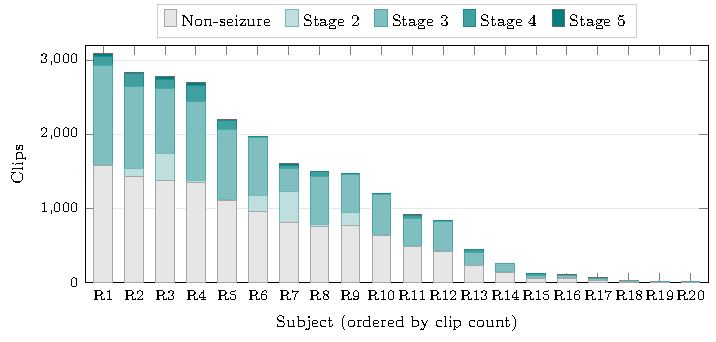
\includegraphics[width=\linewidth]{fig/fig_cohortdist.pdf}
\caption{Per-subject clip composition of the pooled cohort (stacked counts from
Table~\ref{tab:cohort}). Seizure burden is severely long-tailed: the four busiest
animals (R1--R4) dwarf the rest, and subject totals span nearly three orders of magnitude
(11--3{,}091 clips). The most severe stages (S4, dark; S5, darkest) form only a
thin sliver on every bar (193 Stage-5 clips in the entire cohort) which is why
fine-grained grading is so hard.}
\label{fig:cohortdist}
\end{figure*}

\subsection{Task and per-stage visual examples}
\label{sec:dataextra:stages}
Figure~\ref{fig:detexample} makes the binary detection task concrete. The top row
is drawn from a non-seizure interval and the bottom row from a seizure of the
\emph{same} rat in the \emph{same} recording session, so camera, cage and lighting
are identical across the pair and any separation the detector achieves has to come
from behavior. This is the matched-negative sampling our clip extraction enforces
throughout (Sec.~\ref{sec:data}), and it is what makes the detection scores of
Sec.~\ref{sec:application} a test of behavior rather than of scene appearance.

\begin{figure*}[t]
\centering
\setlength{\tabcolsep}{1.5pt}
\renewcommand{\arraystretch}{0.5}
\begin{tabular}{@{}ccccc@{}}
\rotatebox{90}{\footnotesize\ non-sz.} &
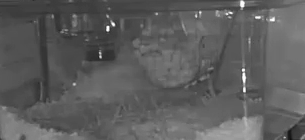
\includegraphics[width=0.22\textwidth]{fig/stages/d_ns_1.png} &
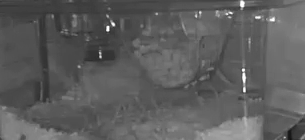
\includegraphics[width=0.22\textwidth]{fig/stages/d_ns_2.png} &
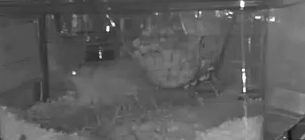
\includegraphics[width=0.22\textwidth]{fig/stages/d_ns_3.png} &
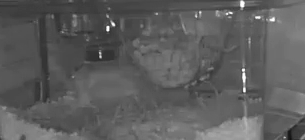
\includegraphics[width=0.22\textwidth]{fig/stages/d_ns_4.png} \\
\rotatebox{90}{\footnotesize\ seizure} &
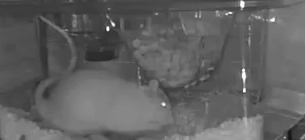
\includegraphics[width=0.22\textwidth]{fig/stages/d_sz_1.png} &
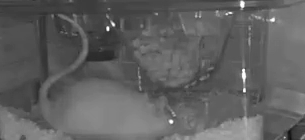
\includegraphics[width=0.22\textwidth]{fig/stages/d_sz_2.png} &
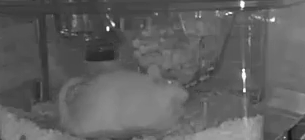
\includegraphics[width=0.22\textwidth]{fig/stages/d_sz_3.png} &
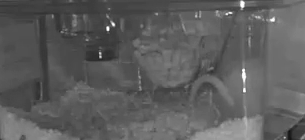
\includegraphics[width=0.22\textwidth]{fig/stages/d_sz_4.png} \\
\end{tabular}
\caption{The binary detection task, visualized. Four frames sampled across a
non-seizure interval (top) and across a seizure (bottom) of the \emph{same} rat in
the \emph{same} recording session, so camera, cage and lighting are identical
across the pair and the detector must separate the two from behavior alone.
De-identified clips.}
\label{fig:detexample}
\end{figure*}

Figure~\ref{fig:stages} shows per-stage seizure \emph{filmstrips}: five frames
sampled across one representative clip for each Racine stage (rows S2--S5), time
increasing left to right. The behavioral signal becomes progressively more overt
with stage, from the subtle movements of Stage\,2, through rearing at
Stage\,3--4, to the pronounced convulsive motion of Stage\,5. This visual progression is the cue a video model reads directly and that a single
EEG channel cannot see, and it underlies video's graceful degradation on the
grading task (Sec.~\ref{sec:application}). All frames are from de-identified clips,
cropped to remove cage-side identifiers.

\begin{figure*}[t]
\centering
\setlength{\tabcolsep}{1.5pt}
\renewcommand{\arraystretch}{0.6}
\begin{tabular}{@{}c ccccc@{}}
\rotatebox{90}{\footnotesize\ \ Stage 2} &
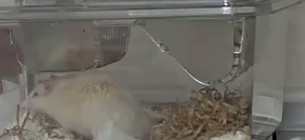
\includegraphics[width=0.187\textwidth]{fig/stages/s2_1.png} &
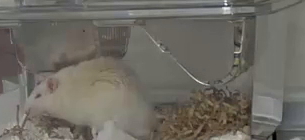
\includegraphics[width=0.187\textwidth]{fig/stages/s2_2.png} &
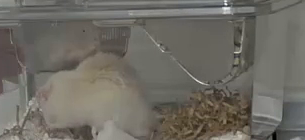
\includegraphics[width=0.187\textwidth]{fig/stages/s2_3.png} &
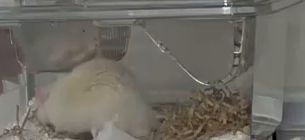
\includegraphics[width=0.187\textwidth]{fig/stages/s2_4.png} &
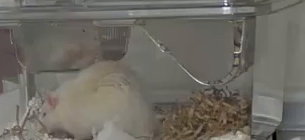
\includegraphics[width=0.187\textwidth]{fig/stages/s2_5.png} \\
\rotatebox{90}{\footnotesize\ \ Stage 3} &
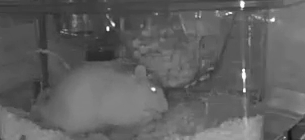
\includegraphics[width=0.187\textwidth]{fig/stages/s3_1.png} &
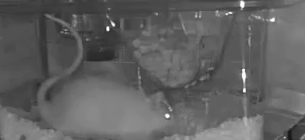
\includegraphics[width=0.187\textwidth]{fig/stages/s3_2.png} &
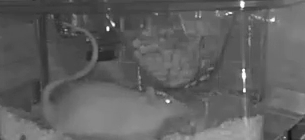
\includegraphics[width=0.187\textwidth]{fig/stages/s3_3.png} &
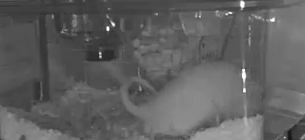
\includegraphics[width=0.187\textwidth]{fig/stages/s3_4.png} &
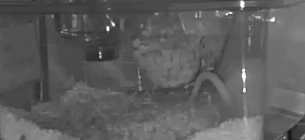
\includegraphics[width=0.187\textwidth]{fig/stages/s3_5.png} \\
\rotatebox{90}{\footnotesize\ \ Stage 4} &
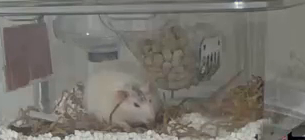
\includegraphics[width=0.187\textwidth]{fig/stages/s4_1.png} &
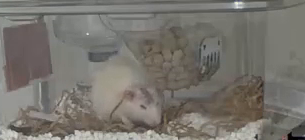
\includegraphics[width=0.187\textwidth]{fig/stages/s4_2.png} &
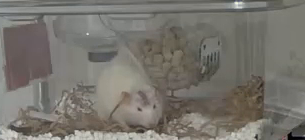
\includegraphics[width=0.187\textwidth]{fig/stages/s4_3.png} &
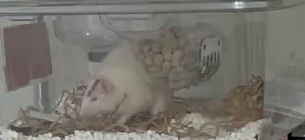
\includegraphics[width=0.187\textwidth]{fig/stages/s4_4.png} &
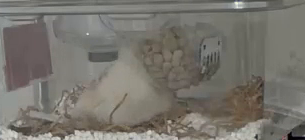
\includegraphics[width=0.187\textwidth]{fig/stages/s4_5.png} \\
\rotatebox{90}{\footnotesize\ \ Stage 5} &
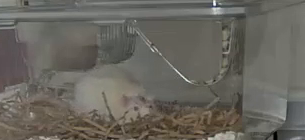
\includegraphics[width=0.187\textwidth]{fig/stages/s5_1.png} &
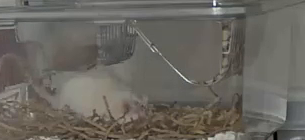
\includegraphics[width=0.187\textwidth]{fig/stages/s5_2.png} &
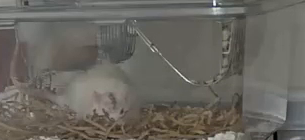
\includegraphics[width=0.187\textwidth]{fig/stages/s5_3.png} &
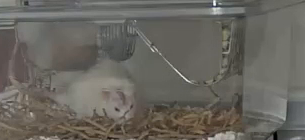
\includegraphics[width=0.187\textwidth]{fig/stages/s5_4.png} &
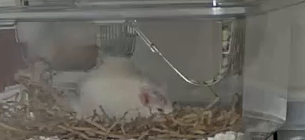
\includegraphics[width=0.187\textwidth]{fig/stages/s5_5.png} \\
 & \multicolumn{5}{c}{\footnotesize time within seizure clip $\longrightarrow$} \\
\end{tabular}
\caption{Per-stage seizure \emph{filmstrips}: five frames sampled across one
representative seizure clip for each Racine stage (rows S2--S5), time increasing
left to right. The behavioral signal grows more overt with stage (from mild
movement at Stage\,2 to pronounced rearing and convulsive motion at Stage\,4--5) which is what a video model reads directly and an EEG channel cannot see. Frames
are from de-identified clips, cropped to remove cage-side identifiers.}
\label{fig:stages}
\end{figure*}

\subsection{Cross-subject appearance variation}
\label{sec:dataextra:crosssubj}
Figure~\ref{fig:crosssubj} shows one frame from each of six animals. Cage
placement, camera framing, illumination (daylight \vs\ infrared) and coat all
differ from animal to animal, because each rat is filmed in its own home cage by
its own fixed camera. This is the appearance shift a model meets when it is tested
on an animal it has never seen, and it is why held-out-\emph{subject}
cross-validation is a harder protocol than held-out-session
(Sec.~\ref{sec:application}). It is also why clips are cropped per cage before
subjects are pooled: without that step a model could separate animals on framing
alone.

\begin{figure}[t]
\centering
\setlength{\tabcolsep}{1.5pt}
\renewcommand{\arraystretch}{0.7}
\begin{tabular}{@{}ccc@{}}
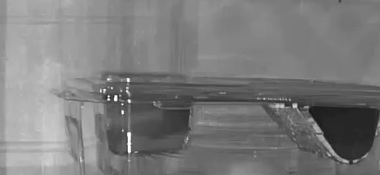
\includegraphics[width=0.31\linewidth]{fig/stages/c_R1.png} &
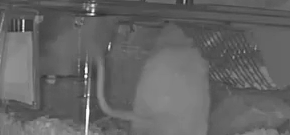
\includegraphics[width=0.31\linewidth]{fig/stages/c_R5.png} &
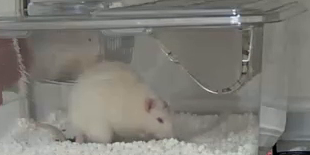
\includegraphics[width=0.31\linewidth]{fig/stages/c_R7.png} \\
{\scriptsize R1} & {\scriptsize R5} & {\scriptsize R7} \\
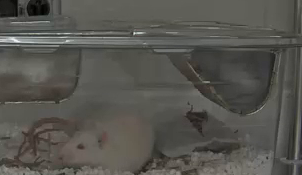
\includegraphics[width=0.31\linewidth]{fig/stages/c_R9.png} &
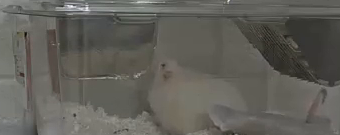
\includegraphics[width=0.31\linewidth]{fig/stages/c_R13.png} &
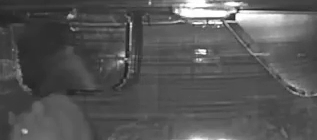
\includegraphics[width=0.31\linewidth]{fig/stages/c_R20.png} \\
{\scriptsize R9} & {\scriptsize R13} & {\scriptsize R20} \\
\end{tabular}
\caption{Cross-subject variation: one frame from six animals (de-identified,
R\,$=$\,subject). Cage placement, camera framing, lighting (daylight \vs\
infrared), and coat differ per animal, part of why held-out-\emph{subject}
generalization is harder than held-out-session, and why the video detector's
stability across subjects (Fig.~\ref{fig:stability}) matters.}
\label{fig:crosssubj}
\end{figure}

\section{Extended Qualitative Results}
\label{sec:qualitative}

This appendix collects the qualitative evidence behind two claims of
Sec.~\ref{sec:application}: where the video detector fails, and what it attends to
when it succeeds.

\subsection{Failure cases}
\label{sec:qualitative:failures}
Figure~\ref{fig:hardcases} shows the two regimes that account for most of the
residual error. The first is the subtle end of the severity scale: a Stage\,2 clip
whose only motion is a brief twitch is hard to separate from ordinary cage
behavior. The second is data scarcity: the near-silent animals at the bottom of
Table~\ref{tab:cohort} contribute only a handful of validation clips each, often
under low-light infrared capture, so their per-subject scores rest on very little
evidence. Both regimes are properties of the cohort rather than of the backbone,
which is why we pair every pooled score with a per-subject breakdown
(Sec.~\ref{sec:problem}).

\begin{figure}[t]
\centering
\setlength{\tabcolsep}{2pt}
\renewcommand{\arraystretch}{0.5}
\begin{tabular}{@{}cc@{}}
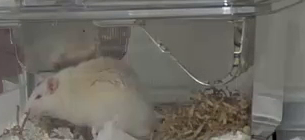
\includegraphics[width=0.47\linewidth]{fig/stages/g_subtle.png} &
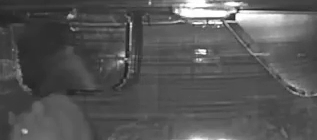
\includegraphics[width=0.47\linewidth]{fig/stages/g_silent.png} \\
{\footnotesize (a) Subtle Stage\,2 (little motion)} & {\footnotesize (b) Near-silent subject (few clips)} \\
\end{tabular}
\caption{Where video is hardest. \emph{(a)}~A Stage\,2 clip with only subtle
movement, easily confused with normal behavior. \emph{(b)}~A near-silent subject
(bottom rows of Table~\ref{tab:cohort}, App.~\ref{sec:dataextra}) with few
validation clips and low-light infrared capture. Rare mild events and data-poor
animals drive most of the residual error. De-identified clips.}
\label{fig:hardcases}
\end{figure}

\subsection{Grad-CAM interpretability}
\label{sec:qualitative:gradcam}
This subsection extends the Grad-CAM~\cite{selvaraju2017gradcam} evidence of
Sec.~\ref{sec:rq1}, where Fig.~\ref{fig:gradcam} shows seizure-class activation
concentrating on the animal's body throughout a Stage\,4 convulsion while staying
diffuse on a non-seizure clip. Because
negatives are sampled from the same sessions as positives
(Sec.~\ref{sec:data}), a detector keying on cage background or recording-setup cues
would produce similar maps for the two, so the contrast is evidence that the model
reads behavior. Figure~\ref{fig:gradcamstages} repeats the check across Stages 2, 3
and 5 and finds the same pattern, so the result is not an artifact of one clip or
one severity level.


\begin{figure*}[t]
\centering
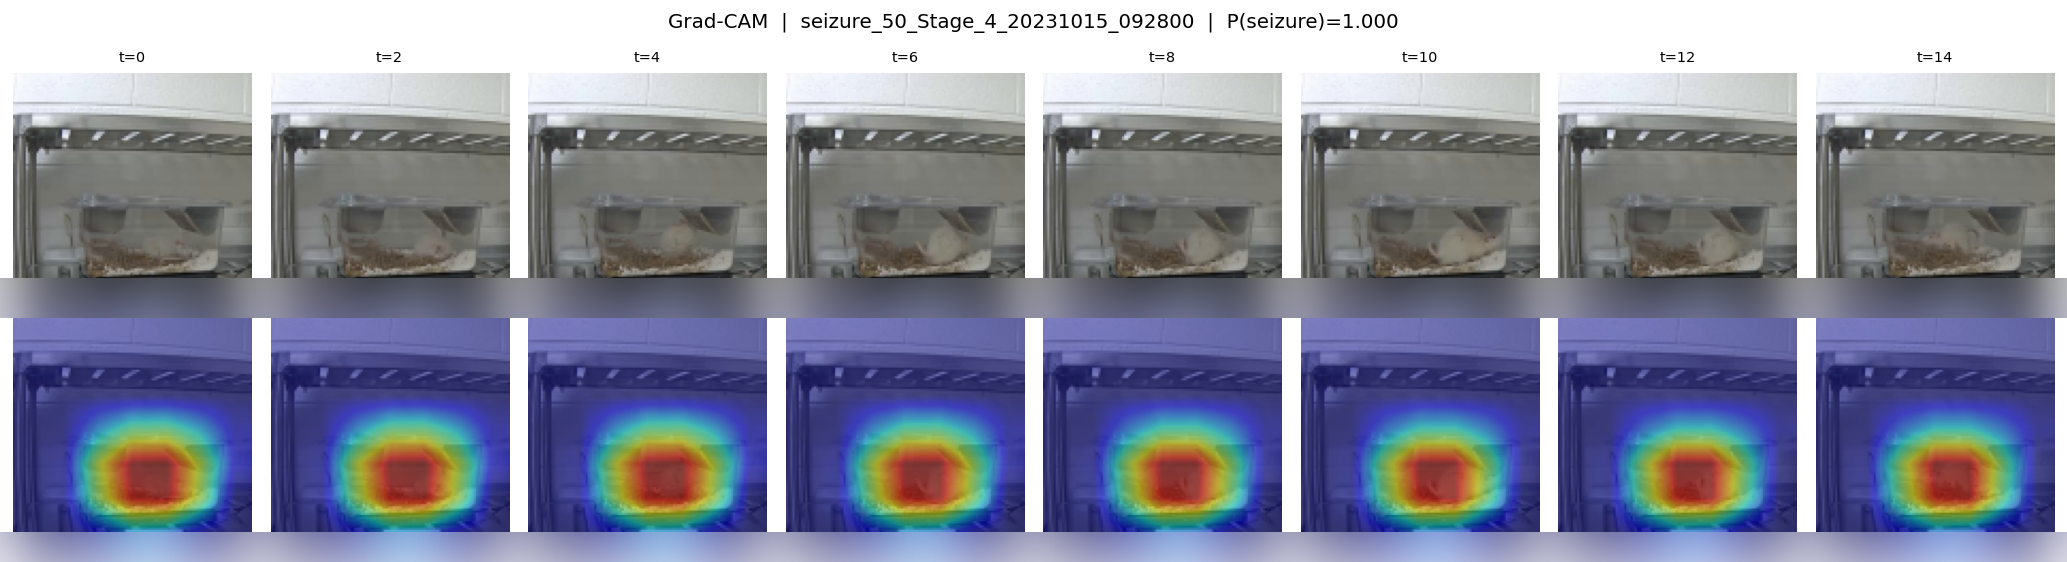
\includegraphics[width=0.98\linewidth, trim=0 0 0 42, clip]{fig/gradcam_stage4_deid.png}\\[1pt]
{\footnotesize (a) Seizure clip (Stage\,4): activation concentrates on the animal}\\[4pt]
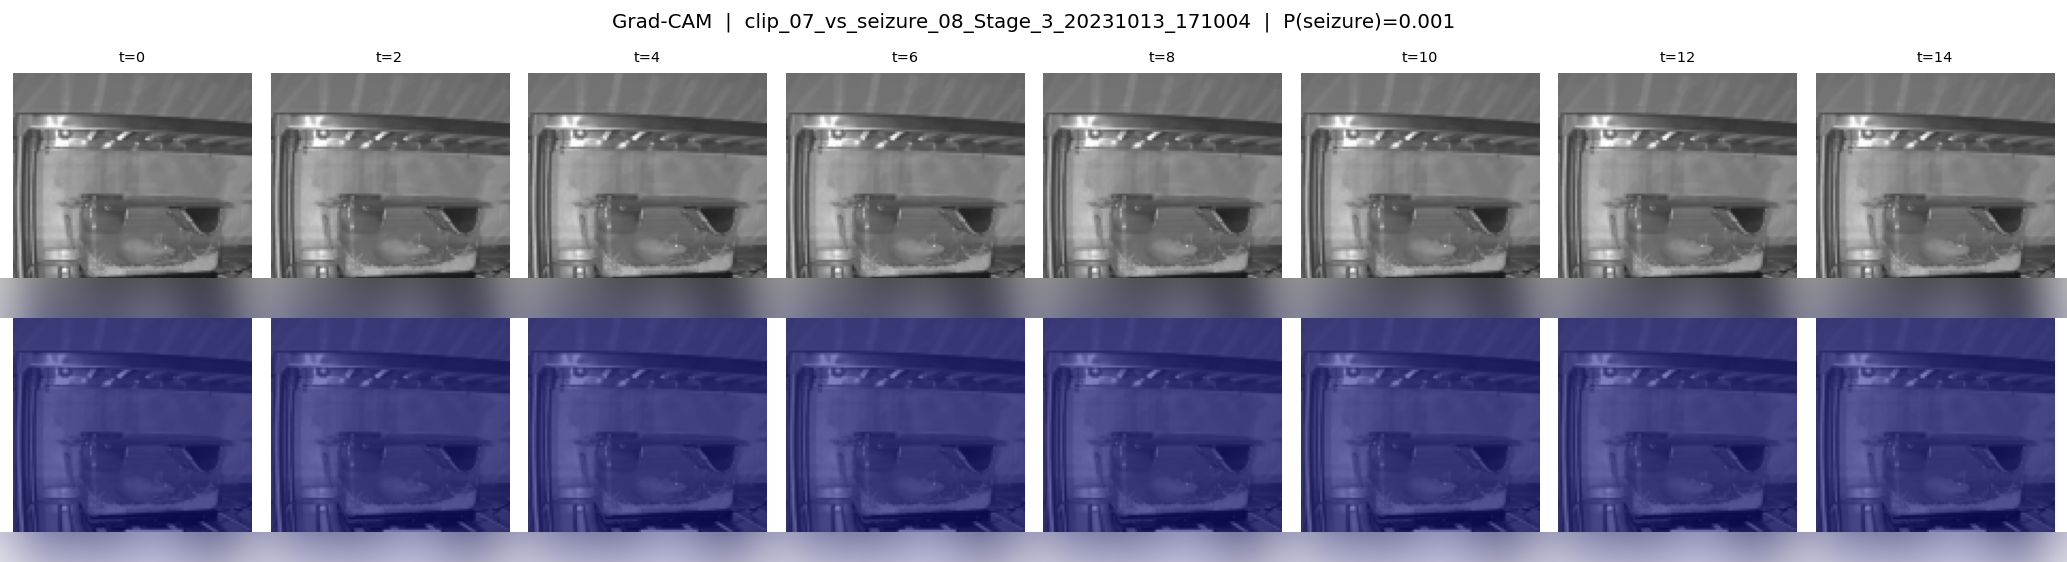
\includegraphics[width=0.98\linewidth, trim=0 0 0 42, clip]{fig/gradcam_nonseizure_deid.png}\\[1pt]
{\footnotesize (b) Non-seizure clip: activation is diffuse, with no focus on the animal}
\caption{Full-width version of Fig.~\ref{fig:gradcam}: all eight sampled frames for
the same two clips, with input frames (top) and seizure-class activation (bottom) in
each strip. De-identified clips; identifier bands redacted.}
\label{fig:gradcamfull}
\end{figure*}

\begin{figure*}[t]
\centering
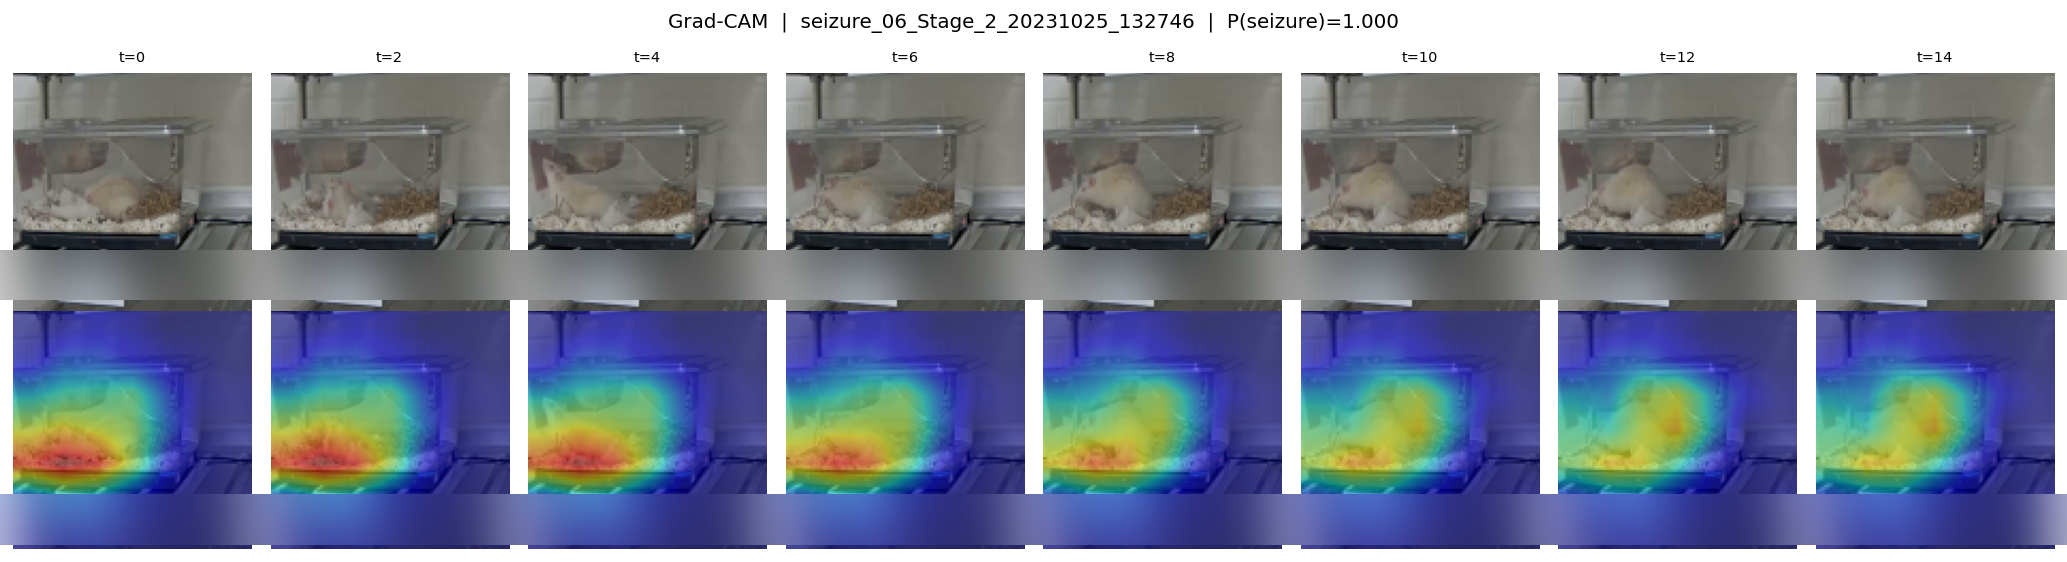
\includegraphics[width=0.98\linewidth, trim=0 0 0 42, clip]{fig/gc_e_s2_deid.png}\\[1pt]
{\footnotesize (a) Stage 2}\\[4pt]
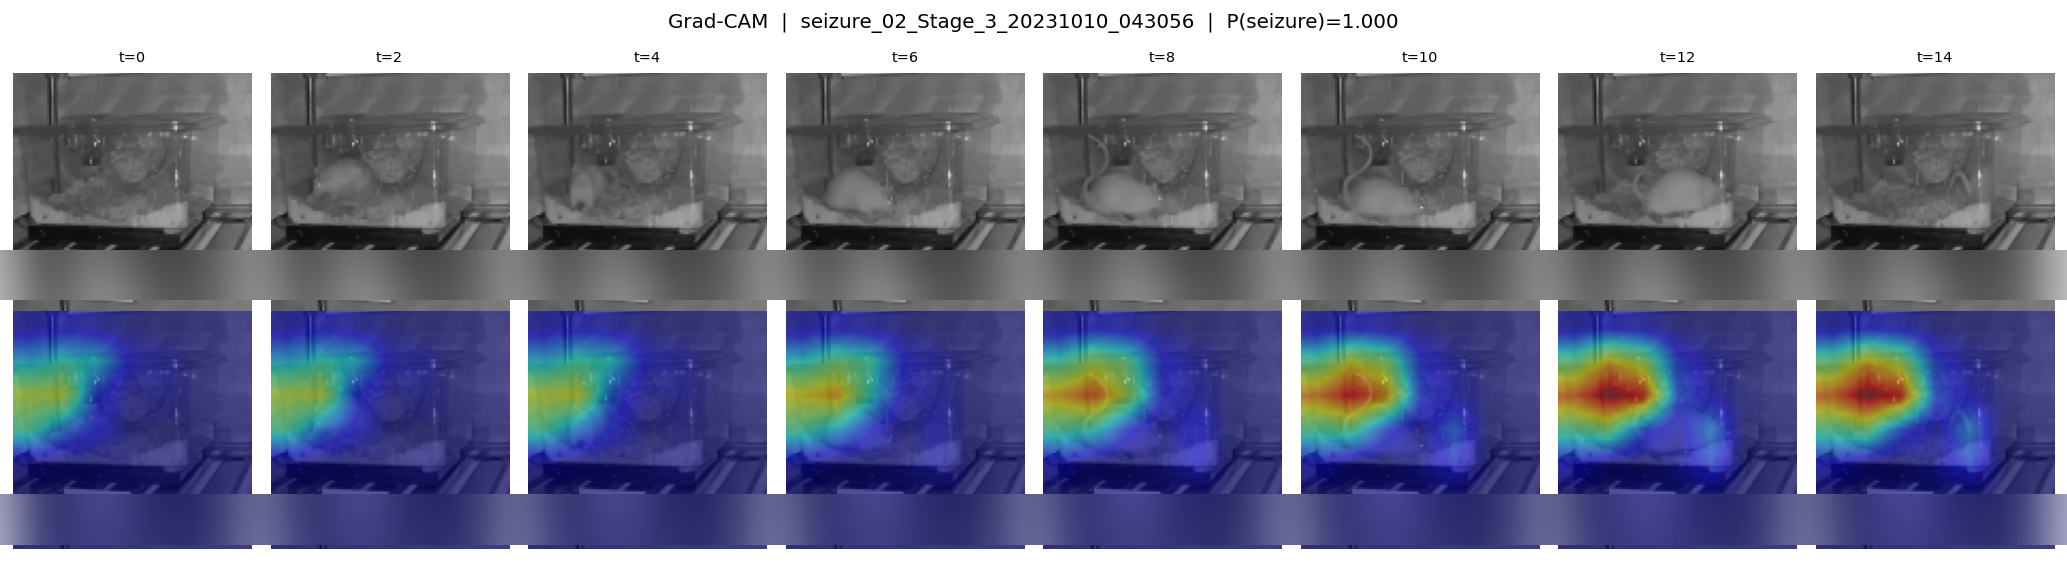
\includegraphics[width=0.98\linewidth, trim=0 0 0 42, clip]{fig/gc_e_s3_deid.png}\\[1pt]
{\footnotesize (b) Stage 3}\\[4pt]
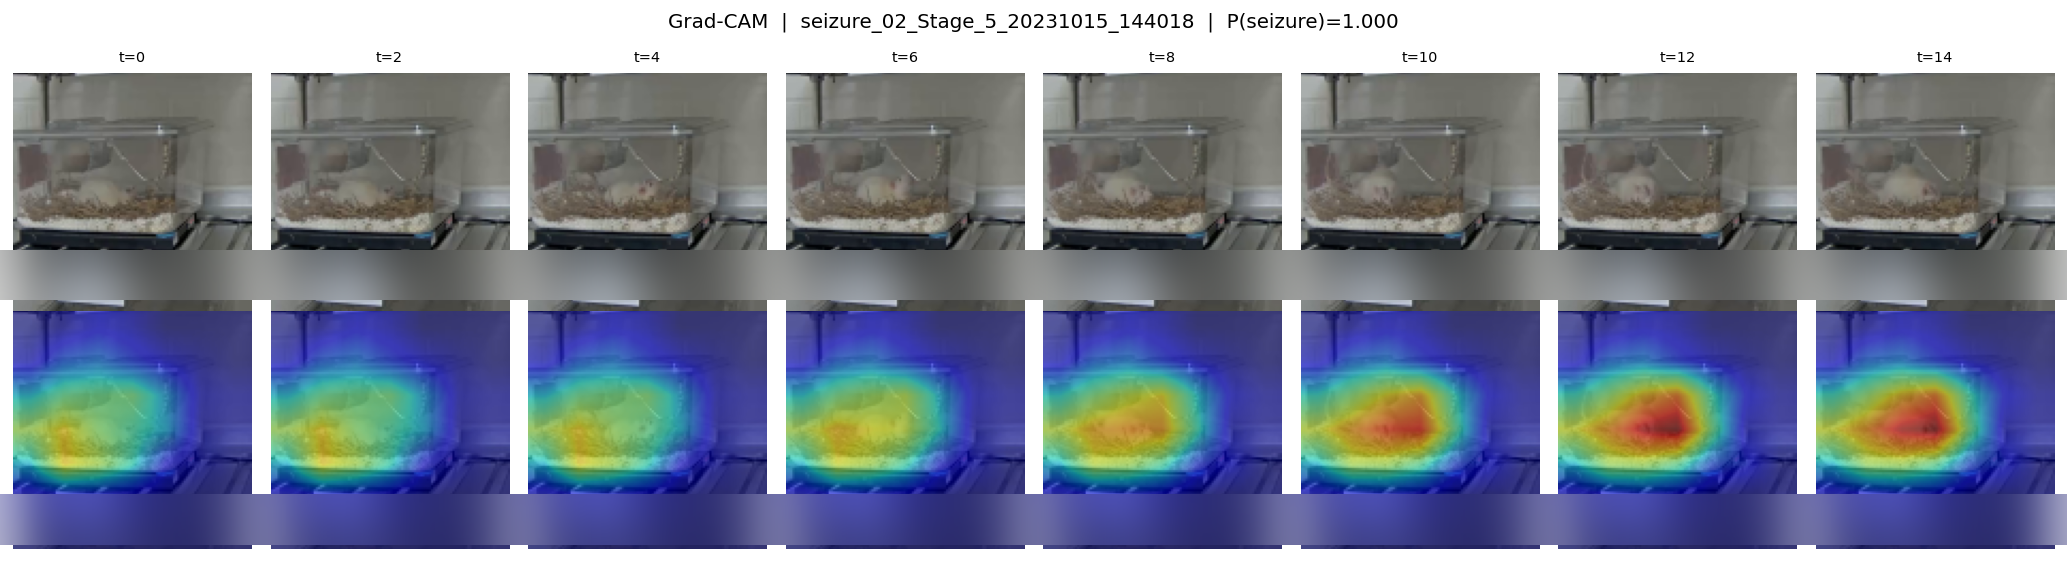
\includegraphics[width=0.98\linewidth, trim=0 0 0 42, clip]{fig/gc_e_s5_deid.png}\\[1pt]
{\footnotesize (c) Stage 5}
\caption{Grad-CAM across severity stages for the R(2+1)D detector; each strip shows
input frames (top) and seizure-class activation (bottom). Activation concentrates
on the animal consistently across Stages 2, 3 and 5, indicating the interpretability
finding is not specific to one clip or stage. De-identified clips (identifier bands
redacted).}
\label{fig:gradcamstages}
\end{figure*}

\subsection{What the shortcut evidence does and does not establish}
\label{sec:qualitative:shortcuts}
Sec.~\ref{sec:rq1} sets out the controls that bound the risk of the detector reading
a shortcut rather than behavior. This subsection states their limits.

The structural arguments exclude particular shortcuts (fixed scene content, cage
framing, static appearance) yet they cannot exclude cues we did not think to
control, such as bedding displacement or a subject-specific motion signature that
correlates with seizure burden. Grad-CAM is weaker evidence still: it shows where
gradient magnitude concentrates, which is suggestive of what the model attends to, short of a causal account of what it uses. The strongest indirect check available
to us is the subject-disjoint protocol of Sec.~\ref{sec:crossmodal}, where a detector
leaning on animal identity should degrade sharply on unseen animals and instead gives
up only 0.022 macro-F1 at detection. Settling the question would take interventions
we have not run (masking the animal, shuffling frame order, or training on
background crops) and we regard those as the natural next test, and do not treat the matter as closed.

\section{Extended Quantitative Results}
\label{sec:extraresults}

This appendix holds two result sets summarized in the main paper: how detection
accuracy scales with the training budget and with pretraining
(Sec.~\ref{sec:rq1}), and the full ten-backbone sweep on the external RodEpil
benchmark (Sec.~\ref{sec:crossmodal}).

\subsection{Data efficiency and pretraining}
\label{sec:extraresults:dataeff}

How much of this performance is bought by data and by transfer? Two ablations
(Table~\ref{tab:dataeff}) answer this. First, holding the R(2+1)D backbone fixed
and training on a growing fraction of the subjects, detection \emph{saturates
quickly}: just two animals ($62$ clips) already give 0.79 macro-F1, half the
cohort (ten subjects, $\sim$11k clips) reaches 0.957, and the full set only adds a
further 0.013 to 0.970. The curve is not perfectly monotone (which subjects enter
training matters more than their count, so twelve subjects dip slightly to 0.946
before recovering) but the overall trend is a shallow saturation, indicating the
task is not data-starved at this scale. Second, pretraining helps but is not essential: training the same
backbone from random initialization, with no Kinetics weights, still reaches
0.952 macro-F1, a modest 0.018 below the pretrained 0.970. Kinetics transfer thus
provides a small, consistent boost and is not a prerequisite.

\begin{table}[!ht]
\centering
\caption{Data efficiency and pretraining (R(2+1)D, 2-class detection,
session-disjoint). Top: macro-F1 \vs\ the fraction of training subjects used
(validation set fixed). Bottom: Kinetics-pretrained \vs\ from-scratch. Detection
saturates well before the full cohort, and pretraining adds only $\sim$0.02. MCC
tracks macro-F1 throughout but falls off faster in the low-data regime.}
\label{tab:dataeff}
\setlength{\tabcolsep}{6pt}
\renewcommand{\arraystretch}{1.15}
\begin{tabular}{@{}c c r cc@{}}
\toprule
\textbf{Train subj.} & \textbf{Frac.} & \textbf{Clips} & \textbf{Macro-F1} & \textbf{MCC} \\
\midrule
2   & 0.10 & 62      & 0.790 & 0.583 \\
5   & 0.25 & 1{,}905  & 0.893 & 0.787 \\
10  & 0.50 & 10{,}969 & 0.957 & 0.914 \\
12  & 0.60 & 11{,}832 & 0.946 & 0.892 \\
15  & 0.75 & 16{,}358 & 0.960 & 0.921 \\
20  & 1.00 & 19{,}208 & \textbf{0.970} & \textbf{0.941} \\
\midrule
\multicolumn{5}{@{}l}{\emph{Pretraining} (full cohort):} \\
\multicolumn{3}{@{}l}{Kinetics-pretrained} & \textbf{0.970} & \textbf{0.941} \\
\multicolumn{3}{@{}l}{from scratch (random init)} & 0.952 & 0.903 \\
\bottomrule
\end{tabular}
\end{table}



\subsection{All ten backbones on RodEpil}
\label{sec:extraresults:rodepilbb}

Beyond R(2+1)D we run the full suite on re-encoded RodEpil under the same
subject-wise five-fold protocol and matched budget (Table~\ref{tab:rodepilbb}). Two things stand out. First, the ranking \emph{reshuffles} relative to our cohort
and spreads far wider (0.87--0.99 macro-F1 \vs\ a 0.03 band on our data). R(2+1)D
now leads clearly (0.986) and the multiscale MViTv2 stays competitive (0.946,
third), but the remaining transformers, TimeSformer (0.871), MViT-v1 (0.890) and Video Swin (0.90--0.91), fall behind the convolutional S3D (0.944) and X3D
(0.933). This ordering inverts our cohort's, where MViTv2 topped
(Table~\ref{tab:vidarch}), reinforcing that backbone choice is a second-order,
data-regime-dependent effect rather than a universal ranking. Second, several video backbones
\emph{exceed} the dataset's
reported TimeSformer baseline of 0.97 seizure-F1: our R(2+1)D reaches 0.978 here under the matched 12-epoch budget, and 0.979 in the dedicated run of Table~\ref{tab:rodepil}. This suggests the benchmark is near-solved for strong
motion models. This comparison is indicative rather than strict: the 0.97
reference was reported on the original release under the authors' own training
setup, whereas our numbers use re-encoded clips and a single fixed budget, at
which our own TimeSformer reaches only 0.799 seizure-F1. Two caveats reinforce
this: SlowFast saturates the benchmark (a perfect 1.000, which we flag rather than
celebrate), and the Video Swin and MViTv2 transformers needed a lower learning
rate ($10^{-4}$) than the conv nets to train stably at this budget.

\begin{table}[t]
\centering
\caption{All ten video backbones on re-encoded RodEpil~\cite{rodepil2025}
(subject-wise 5-fold; F1/AUROC are means over folds, MCC is mean\,$\pm$\,std). Convolutional backbones lead and attention
models trail: the reverse of our cohort ranking (Table~\ref{tab:vidarch});
paradigm labels are given in App.~\ref{sec:arch:video}, Table~\ref{tab:vidspec}. $^\dagger$SlowFast saturates the benchmark (flagged, not a genuine separation). Best non-saturated result in \textbf{bold}; the reference is the dataset's reported
TimeSformer (0.97 seizure-F1).}
\label{tab:rodepilbb}
\setlength{\tabcolsep}{4pt}
\renewcommand{\arraystretch}{1.15}
\resizebox{\columnwidth}{!}{%
\begin{tabular}{@{}l c c c c@{}}
\toprule
\textbf{Backbone} & \textbf{Seiz-F1} & \textbf{Macro-F1} & \textbf{AUROC} & \textbf{MCC} \\
\midrule
SlowFast-R50$^\dagger$~\cite{feichtenhofer2019slowfast} & 1.000 & 1.000 & 1.000 & 1.000\,{\scriptsize$\pm$0.000} \\
R(2+1)D-18~\cite{tran2018r2plus1d} & \textbf{0.978} & \textbf{0.986} & \textbf{0.999} & \textbf{0.972}\,{\scriptsize$\pm$0.015} \\
MViTv2-S~\cite{li2022mvitv2} & \underline{0.916} & \underline{0.946} & \underline{0.989} & \underline{0.891}\,{\scriptsize$\pm$0.020} \\
S3D~\cite{xie2018s3d} & 0.912 & 0.944 & 0.991 & 0.889\,{\scriptsize$\pm$0.029} \\
X3D-M~\cite{feichtenhofer2020x3d} & 0.895 & 0.933 & 0.983 & 0.866\,{\scriptsize$\pm$0.010} \\
VideoMAE-B~\cite{tong2022videomae} & 0.874 & 0.919 & 0.982 & 0.839\,{\scriptsize$\pm$0.025} \\
Video Swin-T~\cite{liu2022videoswin} & 0.861 & 0.910 & 0.979 & 0.823\,{\scriptsize$\pm$0.032} \\
Video Swin-S~\cite{liu2022videoswin} & 0.854 & 0.904 & 0.977 & 0.810\,{\scriptsize$\pm$0.031} \\
MViTv1-B~\cite{fan2021mvit} & 0.835 & 0.890 & 0.971 & 0.784\,{\scriptsize$\pm$0.049} \\
TimeSformer~\cite{bertasius2021timesformer} & 0.799 & 0.871 & 0.957 & 0.743\,{\scriptsize$\pm$0.038} \\
\bottomrule
\end{tabular}}
\end{table}


% fig:gradcam and fig:gradcamstages now live in the supplement
% (App. D, sec:qualitative:gradcam); cited from here and from Sec. 6.

\subsection{Backbone, temporal and spatial ablations in detail}
\label{sec:extraresults:ablations}
This subsection expands the summary read-outs of Sec.~\ref{sec:rq1}.

\noindent\textbf{Backbone ranking.}
Within the 0.03 macro-F1 band of Table~\ref{tab:vidarch}, the multiscale MViTv2-S and
the motion-oriented SlowFast top the table (0.974 macro-F1; SlowFast attains the best
AUROC, 0.995), marginally ahead of R(2+1)D and the tiny X3D-M, with TimeSformer
trailing the field. The ranking is dataset-dependent: on RodEpil, R(2+1)D and
TimeSformer are at near-parity (our 0.979 \vs\ the reported 0.97), reinforcing that
once the data regime is fixed, architecture is a second-order factor relative to
modality and preprocessing. The clustering extends to grading, where the 3- and
5-class columns again fall in narrow bands (3-class macro-F1 0.74--0.79, 5-class
0.59--0.67).

\noindent\textbf{Temporal sampling.}
Four frames already recover most of the detection signal (0.940) and eight reach
0.960, after which the curve flattens: 16 frames give 0.970 and 32 give 0.972. Grading follows the same shape one level down: three- and five-class macro-F1 both
climb from 8 to 32 frames (0.763$\to$0.793 and 0.627$\to$0.667). Doubling to 64
returns nothing at detection or 3-class and actively costs at 5-class, where macro-F1
falls to 0.632, a drop spread across all five classes and largest on Stage\,2. Against 32 frames the 16-frame default concedes 0.002 macro-F1 at detection, 0.012 at
3-class and 0.005 at 5-class for half the compute; the detection and 5-class margins
fall inside the seed spread of Table~\ref{tab:results}, so we treat the two budgets
as equivalent.

\noindent\textbf{Spatial resolution.}
Resolution beyond the $112$ default does not help and slightly hurts. Our clips are
only $\sim$300--480\,px native and the seizure signal is coarse whole-body motion, so
the larger settings upsample the recording and spend compute without adding usable
detail. Higher resolutions (512/1024) would upsample further beyond the source and
are not meaningful here.

\begin{table}[tb]
\centering
\caption{Spatial-resolution ablation: R(2+1)D detection at three input sizes
(16 frames, session-disjoint split, seed 42, 10 epochs; batch scaled $16/8/4$). Source clips are only $\sim$300--480\,px, so both larger settings upsample the
recording and accuracy falls monotonically on all three metrics, at AUROC the top
two separate only past the third decimal ($0.9934$ \vs\ $0.9926$). The $448$ run was
stopped by an out-of-memory kill after $8$ of its $10$ epochs; we report its best
checkpoint, so that row is if anything an optimistic bound on the larger setting. Best per column in \textbf{bold}.}
\label{tab:resolution}
\setlength{\tabcolsep}{8pt}
\renewcommand{\arraystretch}{1.12}
\begin{tabular}{@{}c c c c@{}}
\toprule
\textbf{Input size} & \textbf{Macro-F1} & \textbf{AUROC} & \textbf{MCC} \\
\midrule
$112\times112$ (default) & \textbf{0.970} & \textbf{0.993} & \textbf{0.941} \\
$224\times224$           & 0.967 & 0.993 & 0.934 \\
$448\times448$           & 0.952 & 0.988 & 0.904 \\
\bottomrule
\end{tabular}
\end{table}

\begin{table}[tb]
\centering
\caption{Per-class breakdown at 5-class grading, video (R(2+1)D) \vs\ the EEG GRU
($n$ is the held-out clip count). Both are strong on the common classes and weak on
the rare high-severity stages, and the failure is sharper for EEG: Stage\,4--5
F1 of 0.20 / 0.12 against video's 0.36 / 0.42. Over all five classes the run-level
MCC is 0.830 for video against 0.702 for EEG. The counts differ slightly between
the two columns because the EEG models were retrained on a regenerated clip corpus,
so the held-out sets are not clip-identical.}
\label{tab:perclass}
\setlength{\tabcolsep}{3.5pt}
\renewcommand{\arraystretch}{1.1}
\resizebox{\columnwidth}{!}{%
\begin{tabular}{@{}l rccc rccc@{}}
\toprule
 & \multicolumn{4}{c}{\textbf{Video}} & \multicolumn{4}{c}{\textbf{EEG}} \\
\cmidrule(lr){2-5}\cmidrule(lr){6-9}
\textbf{Stage} & \textbf{n} & \textbf{P} & \textbf{R} & \textbf{F1} & \textbf{n} & \textbf{P} & \textbf{R} & \textbf{F1} \\
\midrule
non-seizure & 2720 & 0.965 & 0.968 & 0.966 & 2737 & 0.914 & 0.955 & 0.934 \\
Stage\,2    &  220 & 0.681 & 0.650 & 0.665 &  256 & 0.491 & 0.863 & 0.626 \\
Stage\,3    & 2148 & 0.904 & 0.896 & 0.900 & 2064 & 0.867 & 0.717 & 0.785 \\
Stage\,4    &  167 & 0.330 & 0.401 & 0.362 &  229 & 0.268 & 0.162 & 0.202 \\
Stage\,5    &   34 & 0.579 & 0.324 & 0.415 &   33 & 0.074 & 0.364 & 0.123 \\
\bottomrule
\end{tabular}}
\end{table}

\subsection{Where each modality fails, and why}
\label{sec:extraresults:failure}

Table~\ref{tab:perclass} shows \emph{that} the two modalities lose accuracy on
different classes. This subsection asks what the errors look like and what produces
them. Figure~\ref{fig:confusion} gives the full confusion structure at all three
granularities and Figure~\ref{fig:failuremodes} summarises the analysis; every
number below is reproduced by \texttt{analyze\_failures.py} and
\texttt{motion\_vs\_error.py}.

\noindent\textbf{The two failure modes are different in kind.}
Video's errors are overwhelmingly \emph{off-by-one} on the severity scale: $72.4\%$
of them land on an adjacent stage, and the dominant single cell is
Stage\,4\,$\to$\,Stage\,3, which absorbs $95$ of $167$ Stage\,4 clips ($57\%$). Video reliably registers that convulsive motion is occurring and misjudges its
degree. EEG fails in two further ways video does not. First it \emph{loses the event}:
$208$ of $2064$ Stage\,3 clips ($10.1\%$) are classified non-seizure, against $49$ of
$2148$ ($2.3\%$) for video: a four-fold higher miss rate on the commonest seizure
class. Second, when it does fire, its errors do not respect the ordinal scale:
$94$ Stage\,3 clips are predicted Stage\,5 and $42$ Stage\,4 clips are predicted
Stage\,5, so errors of two stages or more account for $44\%$ of EEG's mistakes
against $28\%$ of video's (mean $|\Delta\text{stage}|$ $1.51$ \vs\ $1.30$;
Fig.~\ref{fig:failuremodes}a). A single channel supports a seizure/no-seizure
decision but does not carry a monotone severity axis, so its mistakes are not
near-misses.

\noindent\textbf{The one class EEG wins is the one with almost no behavior.}
At Stage\,2 the ordering reverses: EEG recalls $0.863$ against video's $0.650$
(Fig.~\ref{fig:failuremodes}b). Racine Stage\,2 is head nodding and facial
clonus: the rung of the scale with the least whole-body movement. Restricted to the
$2830$ clips both models scored (Table~\ref{tab:paired}), EEG is the only correct
model on $44$ Stage\,2 clips while video is the only correct model on $7$; at
Stage\,3 the same comparison runs $286$ to $43$ the other way. Video's advantage is
behavioral, and it recedes exactly where the behavior does.

\begin{table}[tb]
\centering
\caption{Paired outcomes on the $2830$ clips present in both models' held-out sets
(5-class; the two sets are not clip-identical, see Table~\ref{tab:perclass}). The
per-class rows count clips where exactly one modality is correct. Stage\,2 is the
only class where EEG-only-correct outnumbers video-only-correct.}
\label{tab:paired}
\setlength{\tabcolsep}{5pt}
\renewcommand{\arraystretch}{1.15}
\begin{tabular}{@{}l c c c@{}}
\toprule
\textbf{True class} & \textbf{n} & \textbf{video only} & \textbf{EEG only} \\
\midrule
non-seizure & 1488 & 73  & 44 \\
Stage\,2    &  192 & 7   & \textbf{44} \\
Stage\,3    & 1062 & \textbf{286} & 43 \\
Stage\,4    &   74 & 27  & 8  \\
Stage\,5    &   14 & 8   & 1  \\
\midrule
\multicolumn{4}{@{}l@{}}{\footnotesize overall: both correct $2161$ ($76.4\%$),
video only $401$ ($14.2\%$),}\\
\multicolumn{4}{@{}l@{}}{\footnotesize EEG only $140$ ($4.9\%$), both wrong $128$ ($4.5\%$)}\\
\bottomrule
\end{tabular}
\end{table}

\noindent\textbf{EEG needs a strong, sustained event.}
Two independent measurements point the same way. The seizure a clip is matched to is
shorter when EEG is wrong than when it is right (median $40.4$\,s \vs\ $45.3$\,s),
while video shows no such dependence ($45.1$\,s \vs\ $44.2$\,s). And splitting each
class at its median clip motion energy (mean absolute frame difference over a
sparse grayscale sample, Table~\ref{tab:motion}) EEG's Stage\,3 recall rises from
$0.537$ to $0.777$ across the split. Since the EEG model never sees the video, motion
energy here is standing in for \emph{event intensity}: vigorous seizures produce both
large movement and a clearer electrographic and autonomic signature. The same split
moves video's Stage\,4 recall from $0.182$ to $0.700$, which is the mechanism behind
the Stage\,4\,$\to$\,Stage\,3 compression above, though that cell rests on only $21$
clips.

\begin{table}[tb]
\centering
\caption{Recall on the low- and high-motion half of each class, split at that class's
median motion energy ($900$ clips sampled from the shared set). Motion energy is the
mean absolute frame difference over $24$ evenly spaced frames at $96\times96$
grayscale, computed over the whole clip including its $10$\,s pre- and post-buffers,
so it is a coarse proxy for how vigorous the seizure was.}
\label{tab:motion}
\setlength{\tabcolsep}{4pt}
\renewcommand{\arraystretch}{1.15}
\begin{tabular}{@{}l c c cc cc@{}}
\toprule
 & & & \multicolumn{2}{c}{\textbf{Video recall}} & \multicolumn{2}{c}{\textbf{EEG recall}} \\
\cmidrule(lr){4-5}\cmidrule(lr){6-7}
\textbf{True class} & \textbf{n} & \textbf{med.} & \textbf{low} & \textbf{high} & \textbf{low} & \textbf{high} \\
\midrule
non-seizure & 466 & 1.53 & 0.983 & 0.966 & 0.906 & 1.000 \\
Stage\,2    &  58 & 1.57 & 0.655 & 0.586 & 0.966 & 0.862 \\
Stage\,3    & 350 & 1.78 & 0.891 & 0.943 & 0.537 & \textbf{0.777} \\
Stage\,4    &  21 & 2.17 & 0.182 & \textbf{0.700} & 0.182 & 0.000 \\
\bottomrule
\end{tabular}
\end{table}

\noindent\textbf{Two explanations we tested and could not support.}
We report both, because each is the first hypothesis a reader is likely to form. \emph{(i)~Video loses Stage\,2 because the motion is subtle.} This is the natural
reading of the reversal above, but it does not survive measurement: Stage\,2 video
recall is $0.655$ on the low-motion half and $0.586$ on the high, i.e.\ flat and
weakly in the wrong direction (Table~\ref{tab:motion}), and video's errors overall
sit on \emph{higher}-motion clips than its successes (median $1.676$ \vs\ $1.593$). Whatever separates the Stage\,2 clips EEG recovers from those video recovers, our
motion proxy does not capture it. \emph{(ii)~EEG grades poorly because the channel is
mostly ECG.} Nineteen of twenty-one animals are recorded as ECG rather than EEG
(App.~\ref{sec:dataextra:cohort}), which would explain a signal that detects seizures
but does not encode motor severity. The one true-EEG animal in the held-out set,
RN219, does not stand out: detection macro-F1 $0.981$ and 5-class $0.443$, against
$0.963$ and $0.474$ averaged over the fourteen ECG animals, mid-pack at detection and
slightly below average at grading. With $n{=}1$ this cannot refute the hypothesis, but
it does not support it either, and we therefore do not rest any claim on it.

\begin{figure*}[t]
\centering
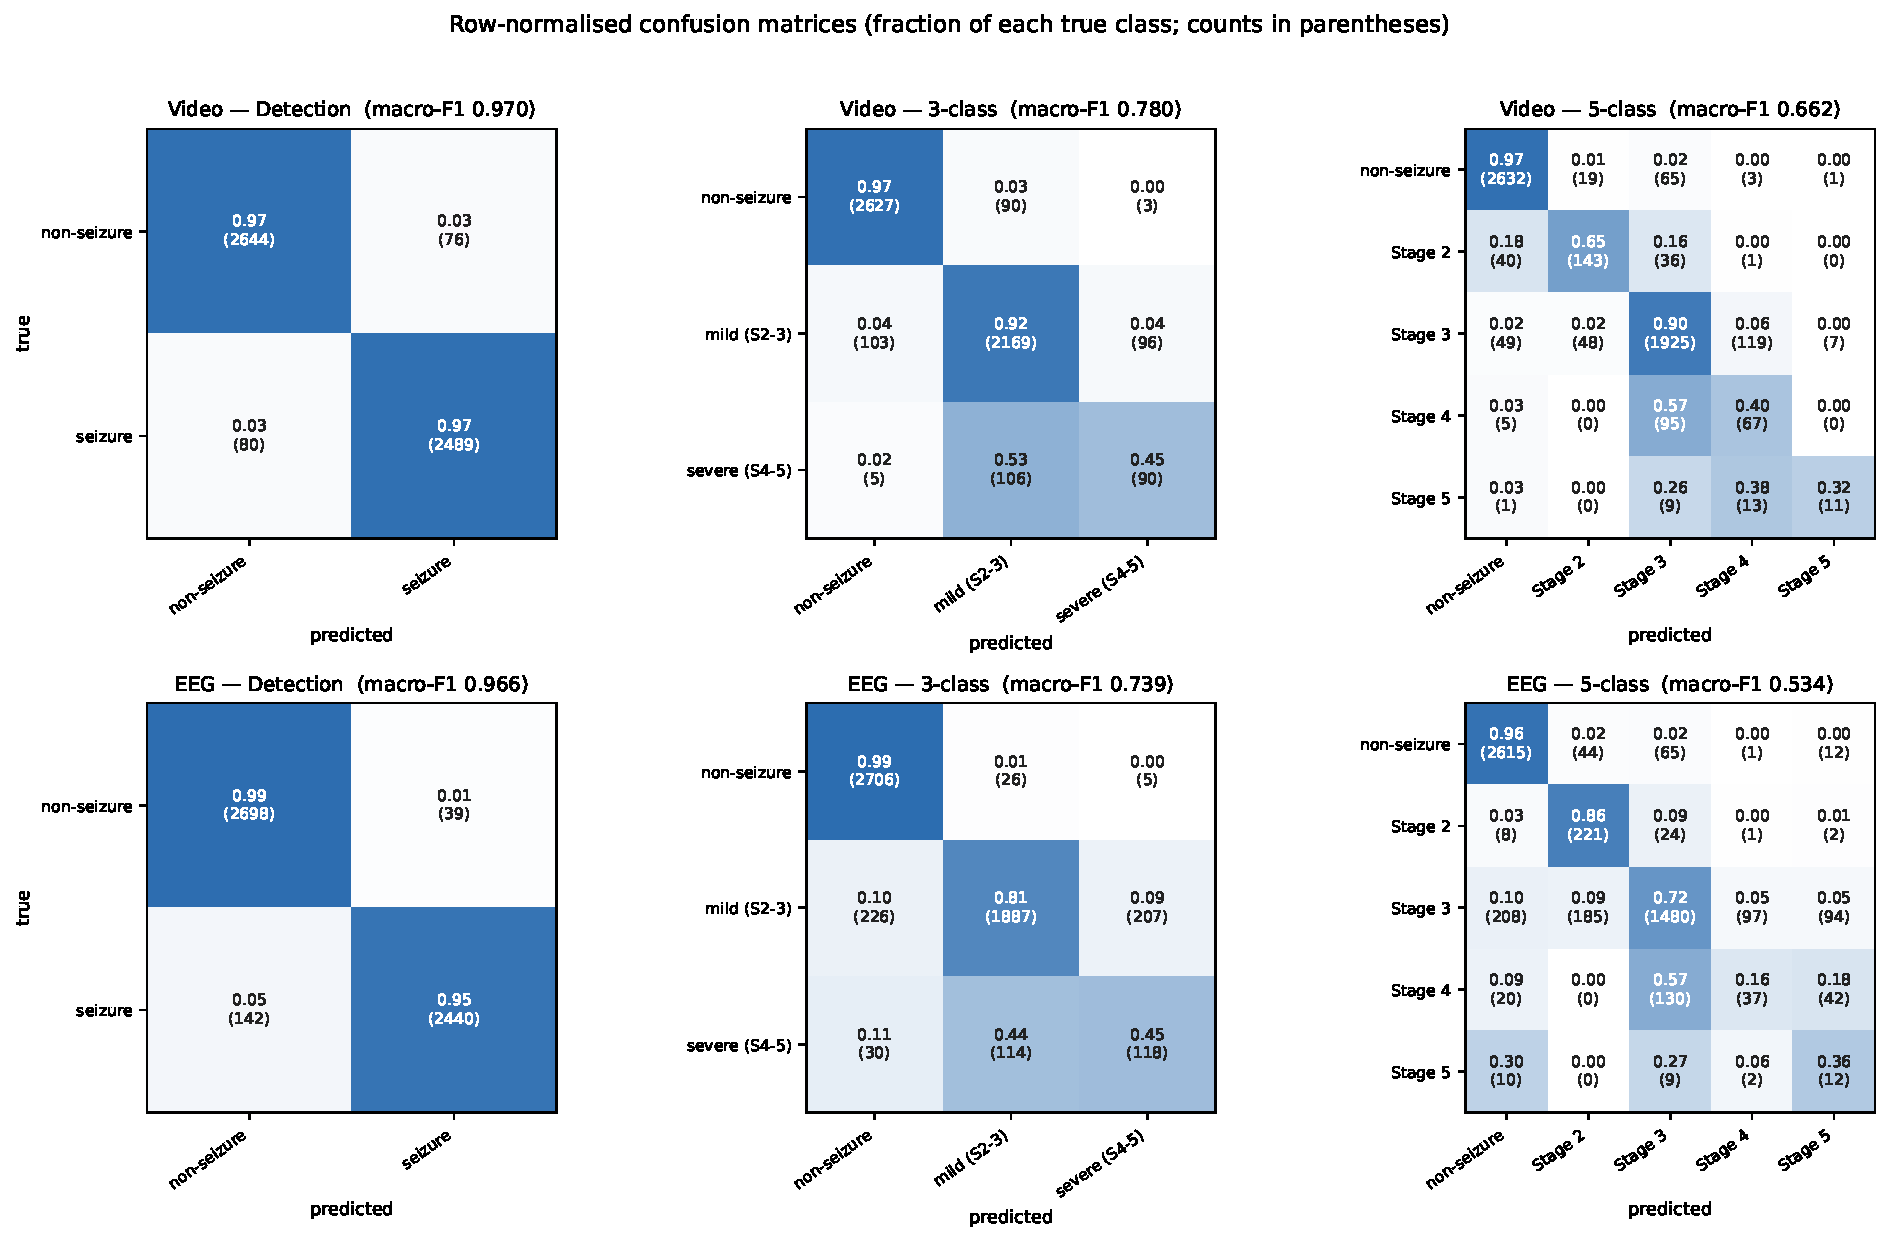
\includegraphics[width=\textwidth]{fig/fig_confusion.pdf}
\caption{Row-normalised confusion matrices for both modalities at all three
granularities (seed-42 runs; fraction of each true class, raw counts in parentheses).
The 5-class panels carry the argument of
App.~\ref{sec:extraresults:failure}: video's mass sits on the sub-diagonal next to
the true class, whereas EEG's leaks both to non-seizure and to non-adjacent stages.}
\label{fig:confusion}
\end{figure*}

\begin{figure*}[t]
\centering
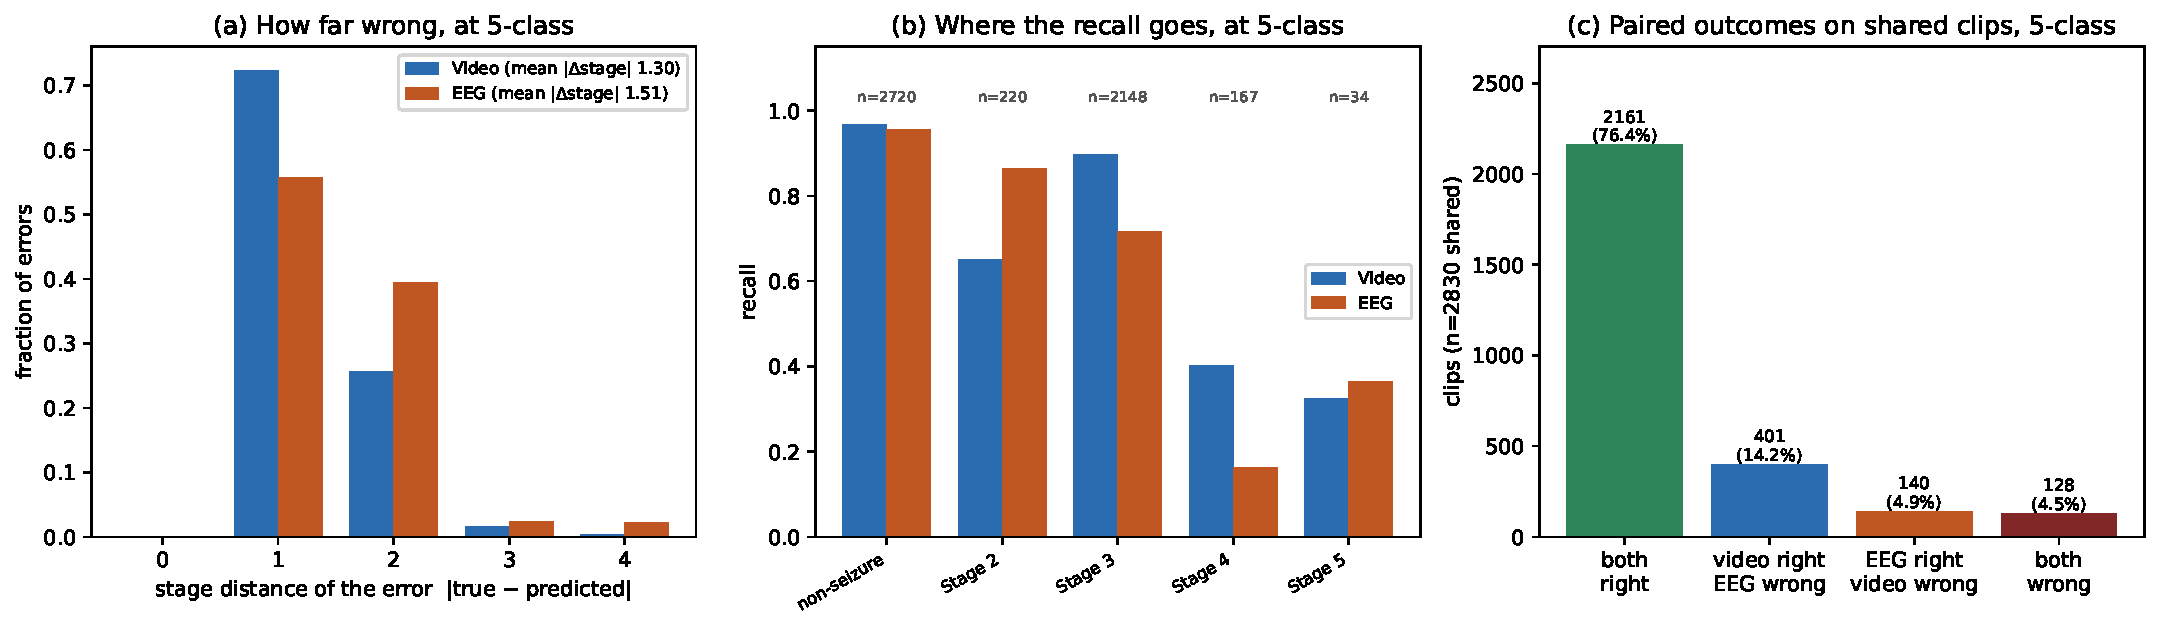
\includegraphics[width=\textwidth]{fig/fig_failure_modes.pdf}
\caption{Error structure at 5-class. \emph{(a)}~Distribution of
$|\text{true}-\text{predicted}|$ over errors: video's are concentrated at one stage,
EEG's spread further (mean $1.30$ \vs\ $1.51$). \emph{(b)}~Per-class recall with
support annotated; the ordering reverses at Stage\,2. \emph{(c)}~Paired outcomes on
the $2830$ clips both models scored.}
\label{fig:failuremodes}
\end{figure*}

\section{Limitations and Future Work in Detail}
\label{sec:openfull}

Sec.~\ref{sec:open} states five limitations in brief. We develop each of them here,
with the evidence from our own results that motivates it.

\noindent\textbf{(1) Cross-subject generalization.}
Seizure burden and per-animal appearance both vary sharply across the cohort
(App.~\ref{sec:dataextra:cohort} and App.~\ref{sec:dataextra:crosssubj}), which makes
held-out-\emph{subject} evaluation the honest test, beyond held-out-session. We
report subject-disjoint five-fold cross-validation on the pooled cohort at all three
granularities (Table~\ref{tab:subjectwise}) and subject-wise folds on
RodEpil~\cite{rodepil2025} (App.~\ref{sec:extraresults:rodepilbb}). Both modalities
hold up at detection: video moves from 0.970 to $0.948\pm0.016$ and the EEG reference
from 0.966 to $0.967\pm0.019$, so neither pooled mean is an artifact of testing on
animals the model has already seen. Two questions stay open. The first is scale: five folds of one cohort cannot settle
transfer across laboratories, species or seizure-induction protocols, and
multi-cohort subject-wise evaluation should become the default here as it already has
in EEG decoding more broadly~\cite{kwon2020subjectindep,xu2020crossdataset}. The
camera-only literature now spans mice~\cite{sabnis2024,khan2024mice}, further rodent
preparations~\cite{epidetect2024,jankovic2019homecage} and even
zebrafish~\cite{whytefagundes2025zebrafish}, so cross-preparation transfer is
testable with data that already exists. The second
is fine-grained severity on unseen animals, the regime where video gives up the most
($0.662$ to $0.475\pm0.024$) and the one a deployed screen would actually face.

\noindent\textbf{(2) Severity grading.}
Detection is largely solved; grading is where the headroom is. The error concentrates in the rare severe stages: Stage\,4 and Stage\,5 together account for only 201 of the 5{,}289 validation clips, and video reaches 0.36 and 0.42 per-class F1 on them (Table~\ref{tab:perclass}). Progress here depends less on architecture than on how
those stages are represented and scored. Three directions follow. Targeted collection
of severe events is the most direct and the most expensive. Ordinal-aware objectives
are the cheapest: the flat softmax we use scores a Stage\,2-for-Stage\,5 confusion
exactly as it scores Stage\,2-for-Stage\,3, and the conditional ordinal formulation of
Sec.~\ref{sec:problem:ordinal} drops that assumption without collecting anything new. Fusion is the third, recruiting the amplitude cues in the electrographic trace that a
camera cannot see. The imbalance strategy itself also deserves a controlled
comparison: Sec.~\ref{sec:rq3} reports inverse-frequency-weighted cross-entropy
without contrasting it against unweighted training,
resampling~\cite{chawla2002smote} or a focal objective~\cite{lin2017focal}, a
well-mapped design space~\cite{johnson2019imbalance} that needs no new data;
precision--recall summaries~\cite{saito2015prc} would also suit the rare stages better
than the threshold-free AUROC we report alongside macro-F1. One further caveat
attaches to the target rather than the model: the Racine scale~\cite{racine1972} was
derived from electrically kindled seizures and its transfer to other induction models
is not automatic~\cite{vanerum2019racine}, so some of the residual five-class error is
plausibly annotation variance.

\noindent\textbf{(3) Cross-modal artifact rejection.}
The clinical reason for recording both streams is that each vetoes the other's
artifacts: a grooming bout that mimics an ictal discharge on a single channel is
obvious on camera, and an electrode transient during quiet rest is obvious in the
trace. Computationally that rationale is almost unexploited. The handful of human
systems that fuse both
streams~\cite{aghaei_video_eeg,martini2021,cao2024,vepinet2024} and the two animal
attempts~\cite{mullen2024,eegvfusion2026} all target binary detection, and none is
organized around artifact rejection as the objective. Adaptive, quality-aware
fusion (weighting each stream by its momentary
reliability~\cite{frontiers_fusion2026,multimodal_review2026}) is the natural
mechanism to realize it. We keep the two streams unfused here by design
(Sec.~\ref{sec:problem:flat}), so we report this as future work. One property of our
setup bounds what any such study could conclude from our numbers: the EEG reference is
single-channel, and a richer montage would change both the artifact profile and the
achievable ceiling.

\noindent\textbf{(4) Benchmarks.}
RodEpil~\cite{rodepil2025} provides the first public \emph{video-only} rodent
benchmark (13{,}053 clips, 19 subjects), and our backbone reaches 0.979 subject-wise
F1 on it (App.~\ref{sec:extraresults:rodepilbb}), which indicates the video result is
not an artifact of our particular cohort. A shared \emph{paired} video--EEG animal
benchmark is still missing, and its absence is why the few fusion papers cannot be compared against one another or against their would-be animal successors.
App.~\ref{sec:bottleneck} documents how severely the scarcity of paired, annotated
data constrains the whole field. Extending a RodEpil-style release with synchronized
EEG and stage-level labels is, in our view, the single most valuable contribution
available here; we release a de-identified description of our cohort as a step toward
it.

\noindent\textbf{(5) Real-time and on-device inference.}
Preclinical monitoring runs continuously for weeks or months, so throughput decides
whether a model is usable at all. vEpiNet's 5.7\,min of compute per recorded
hour~\cite{vepinet2024} shows that real-time video--EEG is already feasible in the
human setting. Our backbone-agnostic result points the same way for animals: X3D-M
matches R(2+1)D-18 while using 4M parameters against 33M
(Table~\ref{tab:vidarch}, Fig.~\ref{fig:efficiency}), so a deployable model costs
little accuracy. The streaming problem is what remains. Clip-level inference on
pre-segmented events is a different task from continuous detection over an
unsegmented feed, where the operative metric becomes false positives per recorded
hour, and where a detector must also decide event boundaries rather than receive
them.


\end{document}
